\documentclass[11pt,a4paper]{article}
\usepackage[utf8]{inputenc}
\usepackage[T1]{fontenc}
\usepackage[brazilian]{babel}
\usepackage[margin=2.3cm]{geometry}
\usepackage{graphicx}
\usepackage{booktabs}
\usepackage{array}
\usepackage{xcolor}
\usepackage{hyperref}
\usepackage{caption}
\usepackage{amsmath}
\usepackage{longtable}
\usepackage{float}
\usepackage{enumitem}
\usepackage{multirow}

\hypersetup{
  colorlinks=true,
  linkcolor=blue!50!black,
  urlcolor=blue!50!black,
  citecolor=blue!50!black
}

\title{Detecção de Anomalias em Cabiúnas via AutoML\\
\large Da vibração de mancais ao falso alerta residual:\\
a jornada completa EXP6 --- EXP10c}
\author{Pipeline \texttt{cnn1d\_ae} / AutoML --- projeto \texttt{TesteMLCab}}
\date{Agosto de 2026}

\begin{document}
\maketitle

\begin{abstract}
Este relatório consolida, num único documento e numa única linha de
raciocínio, toda a série de experimentos que vai do primeiro modelo
multivariado com vibração de mancais (\textbf{EXP6}) até o detector final
com falso alerta reduzido em 82\% (\textbf{EXP10c}). A jornada tem duas
fases nitidamente diferentes. Na \textbf{primeira fase (EXP6 $\to$ EXP7,
itens 1--3)}, o objetivo é \emph{cobertura}: sair de 65\% de antecedência
real (26/40 alarmes) para 72,5\% (29/40) -- e, olhando só os alarmes
fisicamente reais (excluindo falhas de sensor disfarçadas de alarme),
90,6\% (29/32) -- às custas de mais falso alerta (0,06\%$\to$1,94\%). Na
\textbf{segunda fase (EXP10 $\to$ EXP10c)}, o objetivo se inverte: sem
tocar no modelo nem perder nenhum alarme já detectado, cortar o falso
alerta residual de 1,94\% para 0,35\% (queda de 82\%) atacando três causas
estruturais distintas, uma de cada vez. Cada etapa é apresentada com o
mesmo roteiro: onde paramos, o que mudou (com esquema visual do
mecanismo), a configuração usada, e o resultado -- tanto do ponto de vista
agregado (contexto geral) quanto do sensor-alvo especificamente (casos
individuais, antes e depois).
\end{abstract}

\tableofcontents
\clearpage

% =====================================================================
\section*{Glossário de termos técnicos}
\addcontentsline{toc}{section}{Glossário de termos técnicos}
\label{sec:glossario}
% =====================================================================

Termos usados ao longo de todo o relatório, com significado estável em
todas as seções -- consulte esta lista sempre que um termo técnico
aparecer sem explicação no meio do texto.

\subsection*{Avaliação e métricas}

\begin{description}[leftmargin=2.6cm, style=nextline]
  \item[OOS (\emph{out-of-sample})] Período de dados que o modelo
    \textbf{nunca viu} durante o treino/ajuste. É a única forma honesta de
    medir se o modelo generaliza: avaliar no mesmo período usado para
    treinar (\emph{in-sample}) pode dar números ótimos só porque o modelo
    memorizou aquele trecho específico, sem aprender um padrão real --
    isso de fato aconteceu numa etapa anterior desta série
    (\texttt{docs/analise\_automl\_exp5.md}, EXP5-v3: dense com 78--82\%
    de acerto in-sample despencou para 53--65\% assim que validado OOS).
    Neste relatório, o corte OOS é sempre \textbf{2025-07-01}: tudo antes
    é treino, tudo depois é avaliação.
  \item[threshold] Limiar de erro de reconstrução (ou score de anomalia)
    acima do qual um ponto é classificado como anômalo. É definido como um
    \textbf{percentil} da distribuição desse erro \emph{no conjunto de
    treino} -- ex.: ``percentil 99,9'' significa que o threshold é o valor
    que deixa 99,9\% dos pontos de treino abaixo dele, então só o 0,1\%
    mais extremo do próprio treino já seria marcado como anômalo se
    ocorresse de novo.
  \item[debounce] Número de pontos \textbf{consecutivos} que precisam
    ultrapassar o threshold para a anomalia ``contar'' como detecção, em
    vez de ruído momentâneo de um único ponto isolado. \texttt{debounce=1}
    aceita qualquer ponto isolado; \texttt{debounce=6} exige 6 pontos
    seguidos acima do threshold.
  \item[hit\_rate] Fração dos alarmes reais (na avaliação OOS) que tiveram
    pelo menos um ponto anômalo detectado dentro de uma janela ao redor do
    horário do alarme ($\pm$24h neste relatório). \textbf{Não distingue}
    detecção antes do alarme (preditivo) de detecção só depois (reativo)
    -- só mede ``detectou ou não'' dentro da janela.
  \item[normal\_alert\_rate (FP, falso alerta/falso positivo)] Fração de
    pontos em operação normal (longe de qualquer alarme real) que o
    modelo marcou como anômalos. É o ``custo'' do detector -- quanto
    maior, mais alertas sem necessidade o operador teria que checar.
  \item[composite\_score / balanced\_score] Nota única que combina
    \texttt{hit\_rate} e \texttt{normal\_alert\_rate} num só número, usada
    para rankear automaticamente milhares de combinações de
    modelo/percentil/debounce. Penaliza falso alerta ao quadrado, mas
    --- como qualquer score agregado --- pode enganar: um candidato pode
    vencer no score e ainda assim ser pior na prática (ver
    Seção~\ref{sec:licao}).
  \item[seed-sweep (variância de semente)] Reajuste do mesmo modelo
    vencedor várias vezes, mudando só a semente aleatória
    (\emph{random seed}), para checar se o resultado é estável ou se foi
    sorte de uma inicialização específica.
\end{description}

\subsection*{Modelos}

\begin{description}[leftmargin=2.6cm, style=nextline]
  \item[dense] Autoencoder denso (rede neural): aprende a reconstruir o
    vetor de entrada; erro de reconstrução alto = mais anômalo.
  \item[ocsvm (One-Class SVM)] Aprende a fronteira da região ``normal'' no
    espaço de features; a distância até essa fronteira é o score de
    anomalia.
  \item[iforest (Isolation Forest)] Ensemble de árvores de decisão que
    isola pontos aleatoriamente; pontos anômalos são isolados com menos
    cortes (mais fáceis de separar do resto) que pontos normais.
\end{description}

\subsection*{Engenharia de features}

\begin{description}[leftmargin=2.6cm, style=nextline]
  \item[roll\_med / roll\_std / trend\_w / delta\_1] Média móvel, desvio
    padrão móvel, e a diferença entre o valor atual e o valor de
    \texttt{w} passos atrás (tendência) -- todos calculados numa janela de
    tempo específica.
  \item[kurtosis / skewness / crest factor] Estatísticas de \emph{forma}
    da distribuição do sinal numa janela: kurtosis mede o quão
    ``pontiaguda''/pesada é a cauda (picos esporádicos); skewness mede
    assimetria; crest factor é o valor de pico dividido pelo RMS. Ver
    esquema da Seção~\ref{sec:item2}.
  \item[CUSUM / z-score local (\texttt{localz})] Mecanismos que comparam o
    comportamento \emph{recente} do sinal com sua própria linha de base
    histórica (24h), em vez de um limiar fixo global -- pegam um drift
    lento que nunca chega a cruzar um threshold global. Ver esquema da
    Seção~\ref{sec:item3}.
\end{description}

\subsection*{Estado operacional e portões (\emph{gates})}

\begin{description}[leftmargin=2.6cm, style=nextline]
  \item[RUNNING\_A / operational\_state] Sensor de referência que indica
    se a turbina está operando, classificado em \texttt{"on"} (operando
    normalmente), \texttt{"off\_curto"}/\texttt{"off\_longo"} (parada) e
    \texttt{"transiente"} (mudança de estado em andamento). Pontos fora de
    \texttt{"on"} são excluídos tanto do treino quanto da avaliação.
  \item[Portão de rampa / portão de volatilidade (\emph{load gate} /
    \emph{volatility gate})] Mecanismos de pós-processamento que suprimem
    alarmes durante manobras operacionais legítimas (mudança de carga),
    sem alterar o modelo nem o threshold -- ver Parte~\ref{part:exp10}.
\end{description}

\subsection*{Condições de alarme}

\begin{description}[leftmargin=2.6cm, style=nextline]
  \item[HI / HIHI] Alarme de valor alto / muito alto (ex.: temperatura
    acima do normal).
  \item[UNDER] Alarme de valor abaixo do esperado -- no EXP7, descobrimos
    que essa condição específica é, na prática, sempre falha de
    sensor/comunicação, não queda física real (Seção~\ref{sec:qualidade}).
\end{description}

\clearpage
% =====================================================================
\part{Fundamentos: a pipeline e o ponto de partida (EXP6)}
% =====================================================================

% ---------------------------------------------------------------------
\section{Objetivo do EXP6}
% ---------------------------------------------------------------------

A ideia central de toda a série de experimentos deste relatório é usar os
sinais de \textbf{vibração dos 5 mancais} da turbina como preditores
antecipados de falha dos sensores de temperatura \texttt{TC382\_03\_A} e
\texttt{T5\_AVG\_A}. A hipótese física: uma degradação mecânica no mancal
(vibração anormal) pode preceder, em horas, a manifestação térmica que
hoje dispara o alarme -- a vibração funcionaria como sinal de alerta
precoce, antes da temperatura em si sair da faixa normal.

O EXP6 treina um único modelo multivariado que recebe
\texttt{TC382\_03\_A} + \texttt{T5\_AVG\_A} + os 10 canais de vibração como
entrada, mas é avaliado \emph{apenas} pela sua capacidade de antecipar os
alarmes reais desses dois sensores de temperatura -- a vibração entra só
como informação de contexto/apoio (campo \texttt{eval\_sensors}, criado
neste experimento).

% ---------------------------------------------------------------------
\section{Dados e janela temporal}
\label{sec:dados-exp6}
% ---------------------------------------------------------------------

Dataset ClearML \textbf{\texttt{Cabiunas full 2024-2026 30s}}
(\texttt{TesteMLCab}, ID \texttt{a97ba56ba14840fbb1125c2a82f883c9}), usado
em \emph{todos} os experimentos deste relatório (EXP6 até EXP10c):

\begin{itemize}
  \item \texttt{sensores\_full\_2024\_2026\_30s.csv}: 2024-01-01 a
        2026-04-30, resolução de 30s ($\sim$2,45 milhões de linhas), 39
        colunas de sensor.
  \item \texttt{alarmes\_selecionados\_turbina\_a.csv}: 2022-01-04 a
        2026-04-18, 47 tags, 3.757 alarmes onset, sem duplicação de linha.
  \item \textbf{Vibração}: 10 canais \texttt{TV\_35[1-5][X|Y]\_A} (5
        mancais $\times$ radial X/Y) -- disponíveis pela primeira vez
        nesta fonte de dados.
\end{itemize}

\textbf{Janela usada em todos os experimentos:} treino/fit de 2024-07-01 a
2025-06-30 (12 meses); avaliação out-of-sample (OOS) de 2025-07-01 a
2026-04-30 ($\sim$10 meses, 40 alarmes reais de
\texttt{TC382\_03\_A}/\texttt{T5\_AVG\_A}) -- dados e alarmes que o modelo
nunca viu no ajuste.

\begin{figure}[H]
\centering
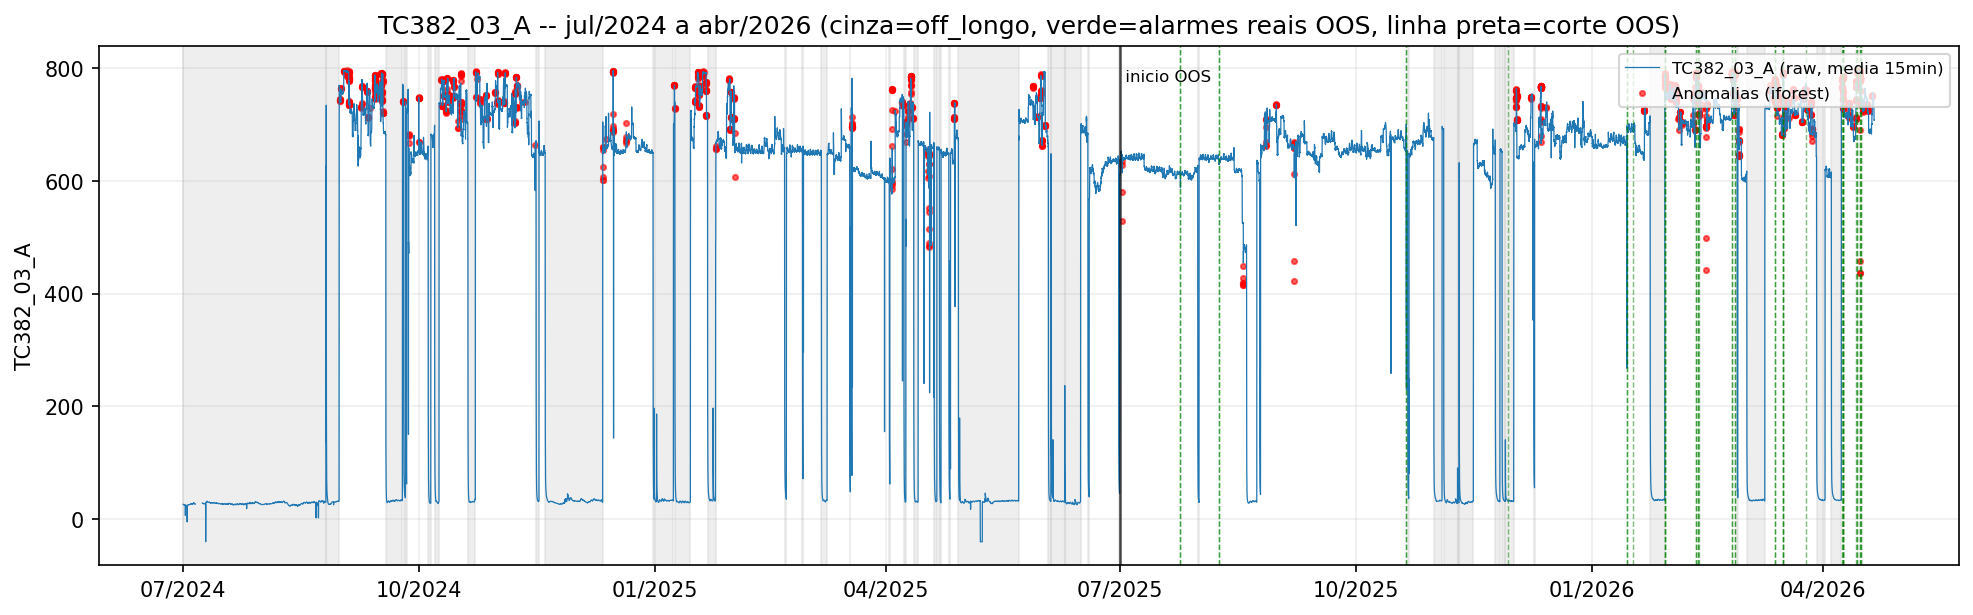
\includegraphics[width=\textwidth]{figs/exp6/00_overview_TC382_03_A.png}
\caption{Série bruta de \texttt{TC382\_03\_A}, jul/2024 a abr/2026. Sombra
cinza = parada prolongada; linha preta vertical = início do período OOS;
linhas verdes tracejadas = alarmes reais no período OOS; pontos vermelhos
= anomalias detectadas pelo modelo final do EXP6.}
\end{figure}

% ---------------------------------------------------------------------
\section{Como a pipeline foi montada}
\label{sec:pipeline}
% ---------------------------------------------------------------------

A pipeline AutoML (\texttt{src/cnn1d\_ae/automl\_pipeline.py}) opera
\textbf{ponto a ponto}: cada instante de tempo é uma amostra de treino
independente, sem janelamento temporal -- diferente do autoencoder CNN-1D
sequencial usado na linha de produção paralela do projeto. Passo a passo,
da entrada bruta até a decisão final:

\begin{enumerate}[leftmargin=*]

\item \textbf{Recorte temporal} (\texttt{DATA\_START\_DATE}): a série
  completa é cortada para o intervalo de interesse antes de qualquer outro
  processamento.

\item \textbf{Normalização do arquivo de alarmes}: mantém só as linhas de
  \emph{onset} (\texttt{Status} iniciando em \texttt{ACT}) -- o arquivo
  traz pares onset/clear para o mesmo evento, e só o onset é algo que faz
  sentido tentar prever com antecedência.

\item \textbf{Construção do dataframe do grupo multivariado}: as colunas
  dos sensores do grupo são unidas por timestamp, com interpolação de
  gaps curtos e \texttt{ffill}/\texttt{bfill} nas bordas.

\item \textbf{Features derivadas} (\texttt{ENABLE\_DERIVED\_FEATURES}):
  para cada sensor, média móvel, desvio móvel e diferença ponto a ponto
  numa janela de tempo -- a granularidade dessa etapa é exatamente o que
  os itens 1 e 2 do EXP7 (Parte~\ref{part:exp7}) vão expandir.

\item \textbf{Estado operacional} (\texttt{OPERATIONAL\_REF\_SENSOR}):
  deriva quando a turbina está \texttt{on}/\texttt{off\_longo}/
  \texttt{off\_curto}/\texttt{transiente} a partir de um sensor de
  referência de operação (\texttt{RUNNING\_A} neste dataset).

\item \textbf{Exclusão do conjunto de treino}: um ponto é excluído do
  treino se estiver perto de um alarme real
  ($\pm$\texttt{EXCLUDE\_MINUTES\_AROUND\_ALARM}), num gap longo de dado,
  ou \textbf{fora do estado \texttt{"on"}} -- ver o achado da
  Seção~\ref{sec:bug-exp6}, que corrige exatamente este ponto.

\item \textbf{Clip de outliers} e \textbf{split temporal OOS}: como já
  descrito -- só dados anteriores ao corte OOS entram no ajuste do modelo.

\item \textbf{Normalização z-score}: estatísticas calculadas somente sobre
  o conjunto de treino, aplicadas a toda a série.

\item \textbf{Ajuste do modelo}: três famílias testadas em paralelo --
  \texttt{dense} (autoencoder Keras), \texttt{ocsvm} (One-Class SVM,
  kernel RBF) e \texttt{iforest} (Isolation Forest).

\item \textbf{Grid de threshold/debounce}: para cada modelo já treinado,
  varre-se um conjunto de percentis de threshold (sobre o erro de
  reconstrução/score de anomalia do treino) $\times$ valores de
  \texttt{debounce} (pontos consecutivos exigidos para contar como
  detecção).

\item \textbf{Avaliação por trial}: \texttt{hit\_rate} (fração de alarmes
  OOS com pelo menos um ponto anômalo dentro de $\pm$24h),
  \texttt{normal\_alert\_rate} (fração de pontos normais marcados como
  anômalos) e o \texttt{composite\_score}:
  \[
  \text{balanced\_score} = \text{hit\_rate} - \text{fp\_penalty} \cdot \text{normal\_alert\_rate}^2
  \]

\item \textbf{\texttt{eval\_sensors}}: sensores que entram só como
  \emph{feature} (a vibração, aqui) não contam alarme próprio no
  \texttt{hit\_rate} -- a avaliação fica restrita a
  \texttt{["TC382\_03\_A", "T5\_AVG\_A"]}.

\end{enumerate}

% ---------------------------------------------------------------------
\section{Achado pré-resultado: a máscara operacional não cobria o treino}
\label{sec:bug-exp6}
% ---------------------------------------------------------------------

Antes de aceitar qualquer resultado, verificamos se as máscaras cobriam de
fato o \emph{treino}, não só a \emph{avaliação}. Encontramos um problema
real: o estado operacional só zerava anomalias na hora de
\textbf{pontuar} -- nunca excluía os períodos desligados do próprio
\textbf{conjunto de treino}. O modelo era ajustado numa mistura de dois
regimes muito diferentes (turbina operando, $\sim$500--800°C, vs. parada,
$\sim$25--40°C).

\textbf{Antes da correção}: \texttt{hit\_rate}=97,5\% mas
\texttt{normal\_alert\_rate}=10,3\% -- o modelo aprendia sobretudo a
detectar a transição liga/desliga, não anomalias sutis em operação. A
correção resolveu de graça outro problema: 99,9\% do platô de sensor
``morto'' em $-40{,}51^{\circ}$C de \texttt{TC382\_03\_A} coincide com
\texttt{RUNNING\_A==0} -- excluir ``não-on'' do treino remove esse
artefato sem mexer no threshold de outlier separadamente.

\textbf{Correção}: o cálculo do estado operacional foi movido para
\emph{antes} da construção do conjunto de treino; \texttt{state != "on"}
passou a ser mais um critério de exclusão do treino, junto com proximidade
de alarme e gaps longos. Todos os resultados a partir daqui já refletem
essa correção -- e ela é o \emph{precursor direto} da máscara operacional
que será estendida no EXP10 (Parte~\ref{part:exp10}).

% ---------------------------------------------------------------------
\section{Configuração da rodada}
% ---------------------------------------------------------------------

\begin{table}[H]
\centering
\small
\begin{tabular}{@{}ll@{}}
\toprule
\textbf{Parâmetro} & \textbf{Valor} \\
\midrule
Grupo & \texttt{TC382\_T5\_vibracao\_mancais} \\
Sensores (features) & \texttt{TC382\_03\_A}, \texttt{T5\_AVG\_A} + 10 canais \texttt{TV\_} \\
\texttt{eval\_sensors} & \texttt{TC382\_03\_A}, \texttt{T5\_AVG\_A} \\
Janela de fit / avaliação OOS & 2024-07 a 2025-06 / 2025-07 a 2026-04 \\
\texttt{OPERATIONAL\_REF\_SENSOR} & \texttt{RUNNING\_A} (\texttt{OFF\_ABS\_THRESHOLD=0.5}) \\
\texttt{ENABLE\_DERIVED\_FEATURES} & \texttt{true} (janela única, 6 min) \\
Grid & 7 percentis $\times$ 6 debounces $\times$ 3 modelos = 126 trials \\
\bottomrule
\end{tabular}
\caption{Configuração completa (\texttt{test\_grupo\_exp6\_vibracao.json}).}
\end{table}

% ---------------------------------------------------------------------
\section{Quem venceu a rodada}
% ---------------------------------------------------------------------

\begin{table}[H]
\centering
\resizebox{\textwidth}{!}{%
\begin{tabular}{@{}lccccc@{}}
\toprule
\textbf{Modelo} & \textbf{Percentil / debounce} & \textbf{hit\_rate} & \textbf{normal\_alert\_rate} & \textbf{anomalias/dia} & \textbf{composite\_score} \\
\midrule
ocsvm (vencedor oficial) & 97,0 / 1 & 97,5\% (39/40) & \textbf{26,15\%} & 730,6 & 0,946 \\
dense & 99,5 / 3 & 82,5\% (33/40) & 12,92\% & 376,4 & 0,931 \\
\textbf{iforest} & \textbf{99,9 / 6} & \textbf{75,0\% (30/40)} & \textbf{0,06\%} & \textbf{3,2} & 0,917 \\
\bottomrule
\end{tabular}%
}
\caption{Melhor trial de cada modelo, dos 126 do grid completo.}
\end{table}

O vencedor pelo \texttt{composite\_score} (\texttt{ocsvm}, 0,946) tem falso
alerta \textbf{436 vezes maior} que o \texttt{iforest} (0,917) -- sinal de
que a penalidade de FP não impede essa escolha quando o \texttt{hit\_rate}
sobe muito. Confirmado visualmente: o \texttt{ocsvm} marca quase toda a
faixa operacional como anômala, sem discriminar nada.

\begin{figure}[H]
\centering
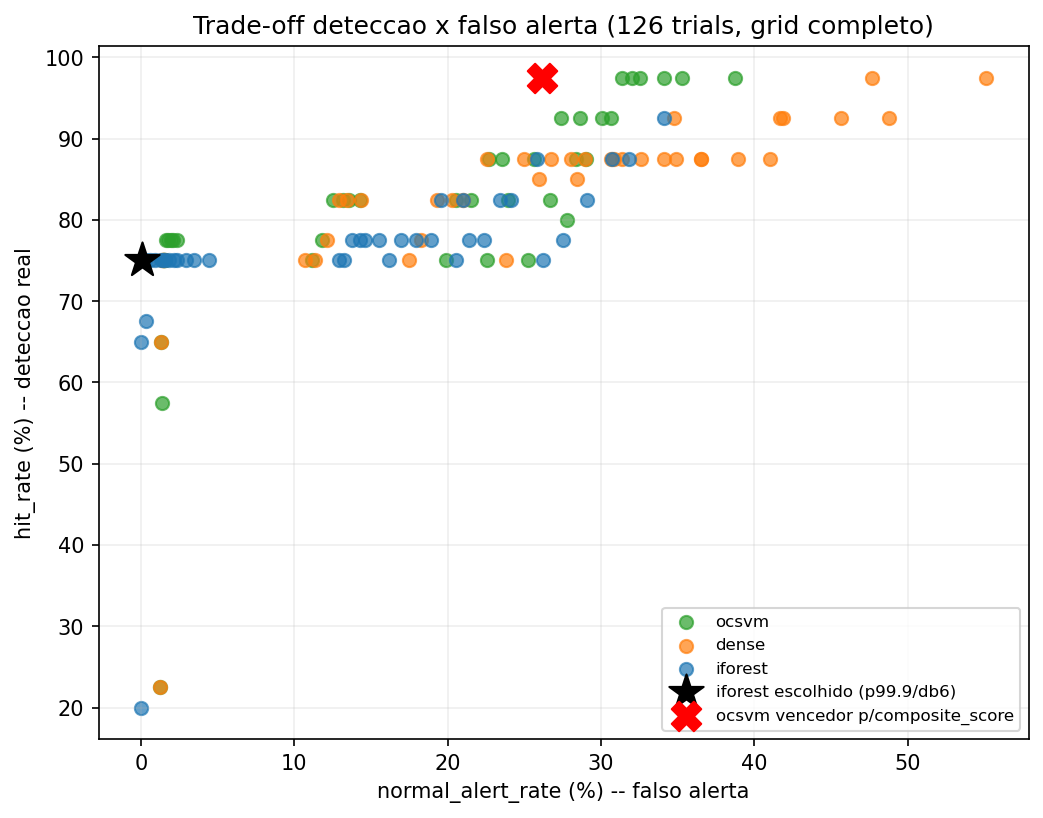
\includegraphics[width=0.85\textwidth]{figs/exp6/03_tradeoff_scatter.png}
\caption{Trade-off detecção $\times$ falso alerta para os 126 trials. O
\texttt{iforest} escolhido (estrela) está no canto ideal
(alta detecção, baixíssimo FP); o \texttt{ocsvm} vencedor pelo score (X)
tem FP muito mais alto para ganho marginal de detecção.}
\end{figure}

\begin{figure}[H]
\centering
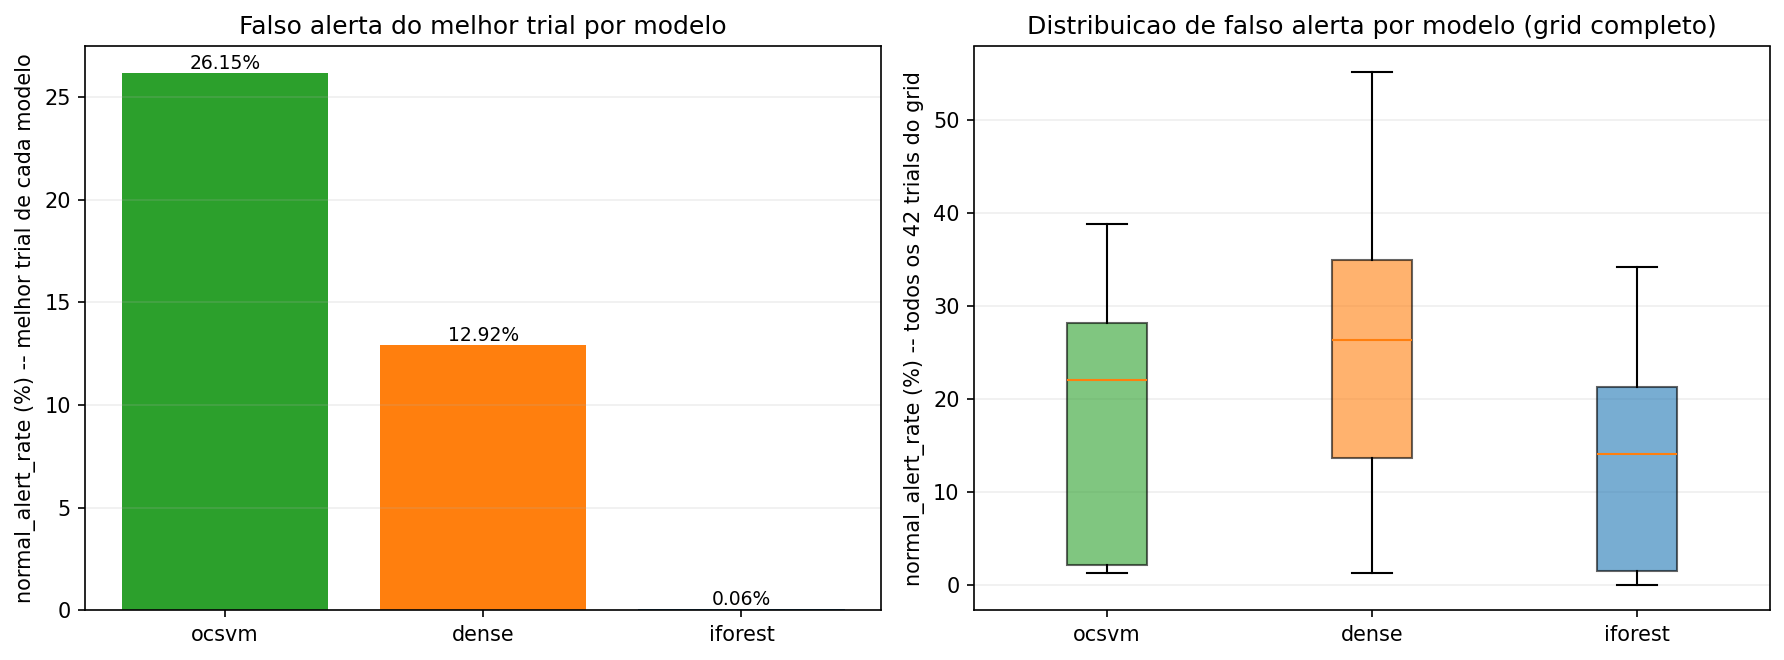
\includegraphics[width=0.95\textwidth]{figs/exp6/02_fp_por_modelo.png}
\caption{Esquerda: falso alerta do melhor trial de cada modelo. Direita:
distribuição de FP considerando todos os 42 trials de cada modelo --
o \texttt{iforest} tem mais configurações de baixo FP disponíveis, não só
o ponto ótimo isolado.}
\end{figure}

\textbf{Candidato prático escolhido: \texttt{iforest} (p99,9/debounce=6)}
-- reproduzido de forma independente numa segunda run isolada, com
métricas e hiperparâmetros idênticos, confirmando reprodutibilidade.

% ---------------------------------------------------------------------
\section{Resultado obtido}
\label{sec:resultado-exp6}
% ---------------------------------------------------------------------

\begin{table}[H]
\centering
\begin{tabular}{@{}lcc@{}}
\toprule
\textbf{Categoria} & \textbf{Qtd.} & \textbf{\% dos 40 alarmes} \\
\midrule
\textbf{Preditivo} (antecedência real) & \textbf{26} & \textbf{65,0\%} \\
Reativo (só depois/simultâneo) & 4 & 10,0\% \\
\textbf{Sem detecção} & \textbf{10} & \textbf{25,0\%} \\
\bottomrule
\end{tabular}
\caption{\texttt{hit\_rate}=75,0\% (30/40); \texttt{normal\_alert\_rate}=0,06\%;
mediana de antecedência (dos 26 preditivos) = 12,4h.}
\label{tab:resultado-exp6}
\end{table}

\begin{figure}[H]
\centering
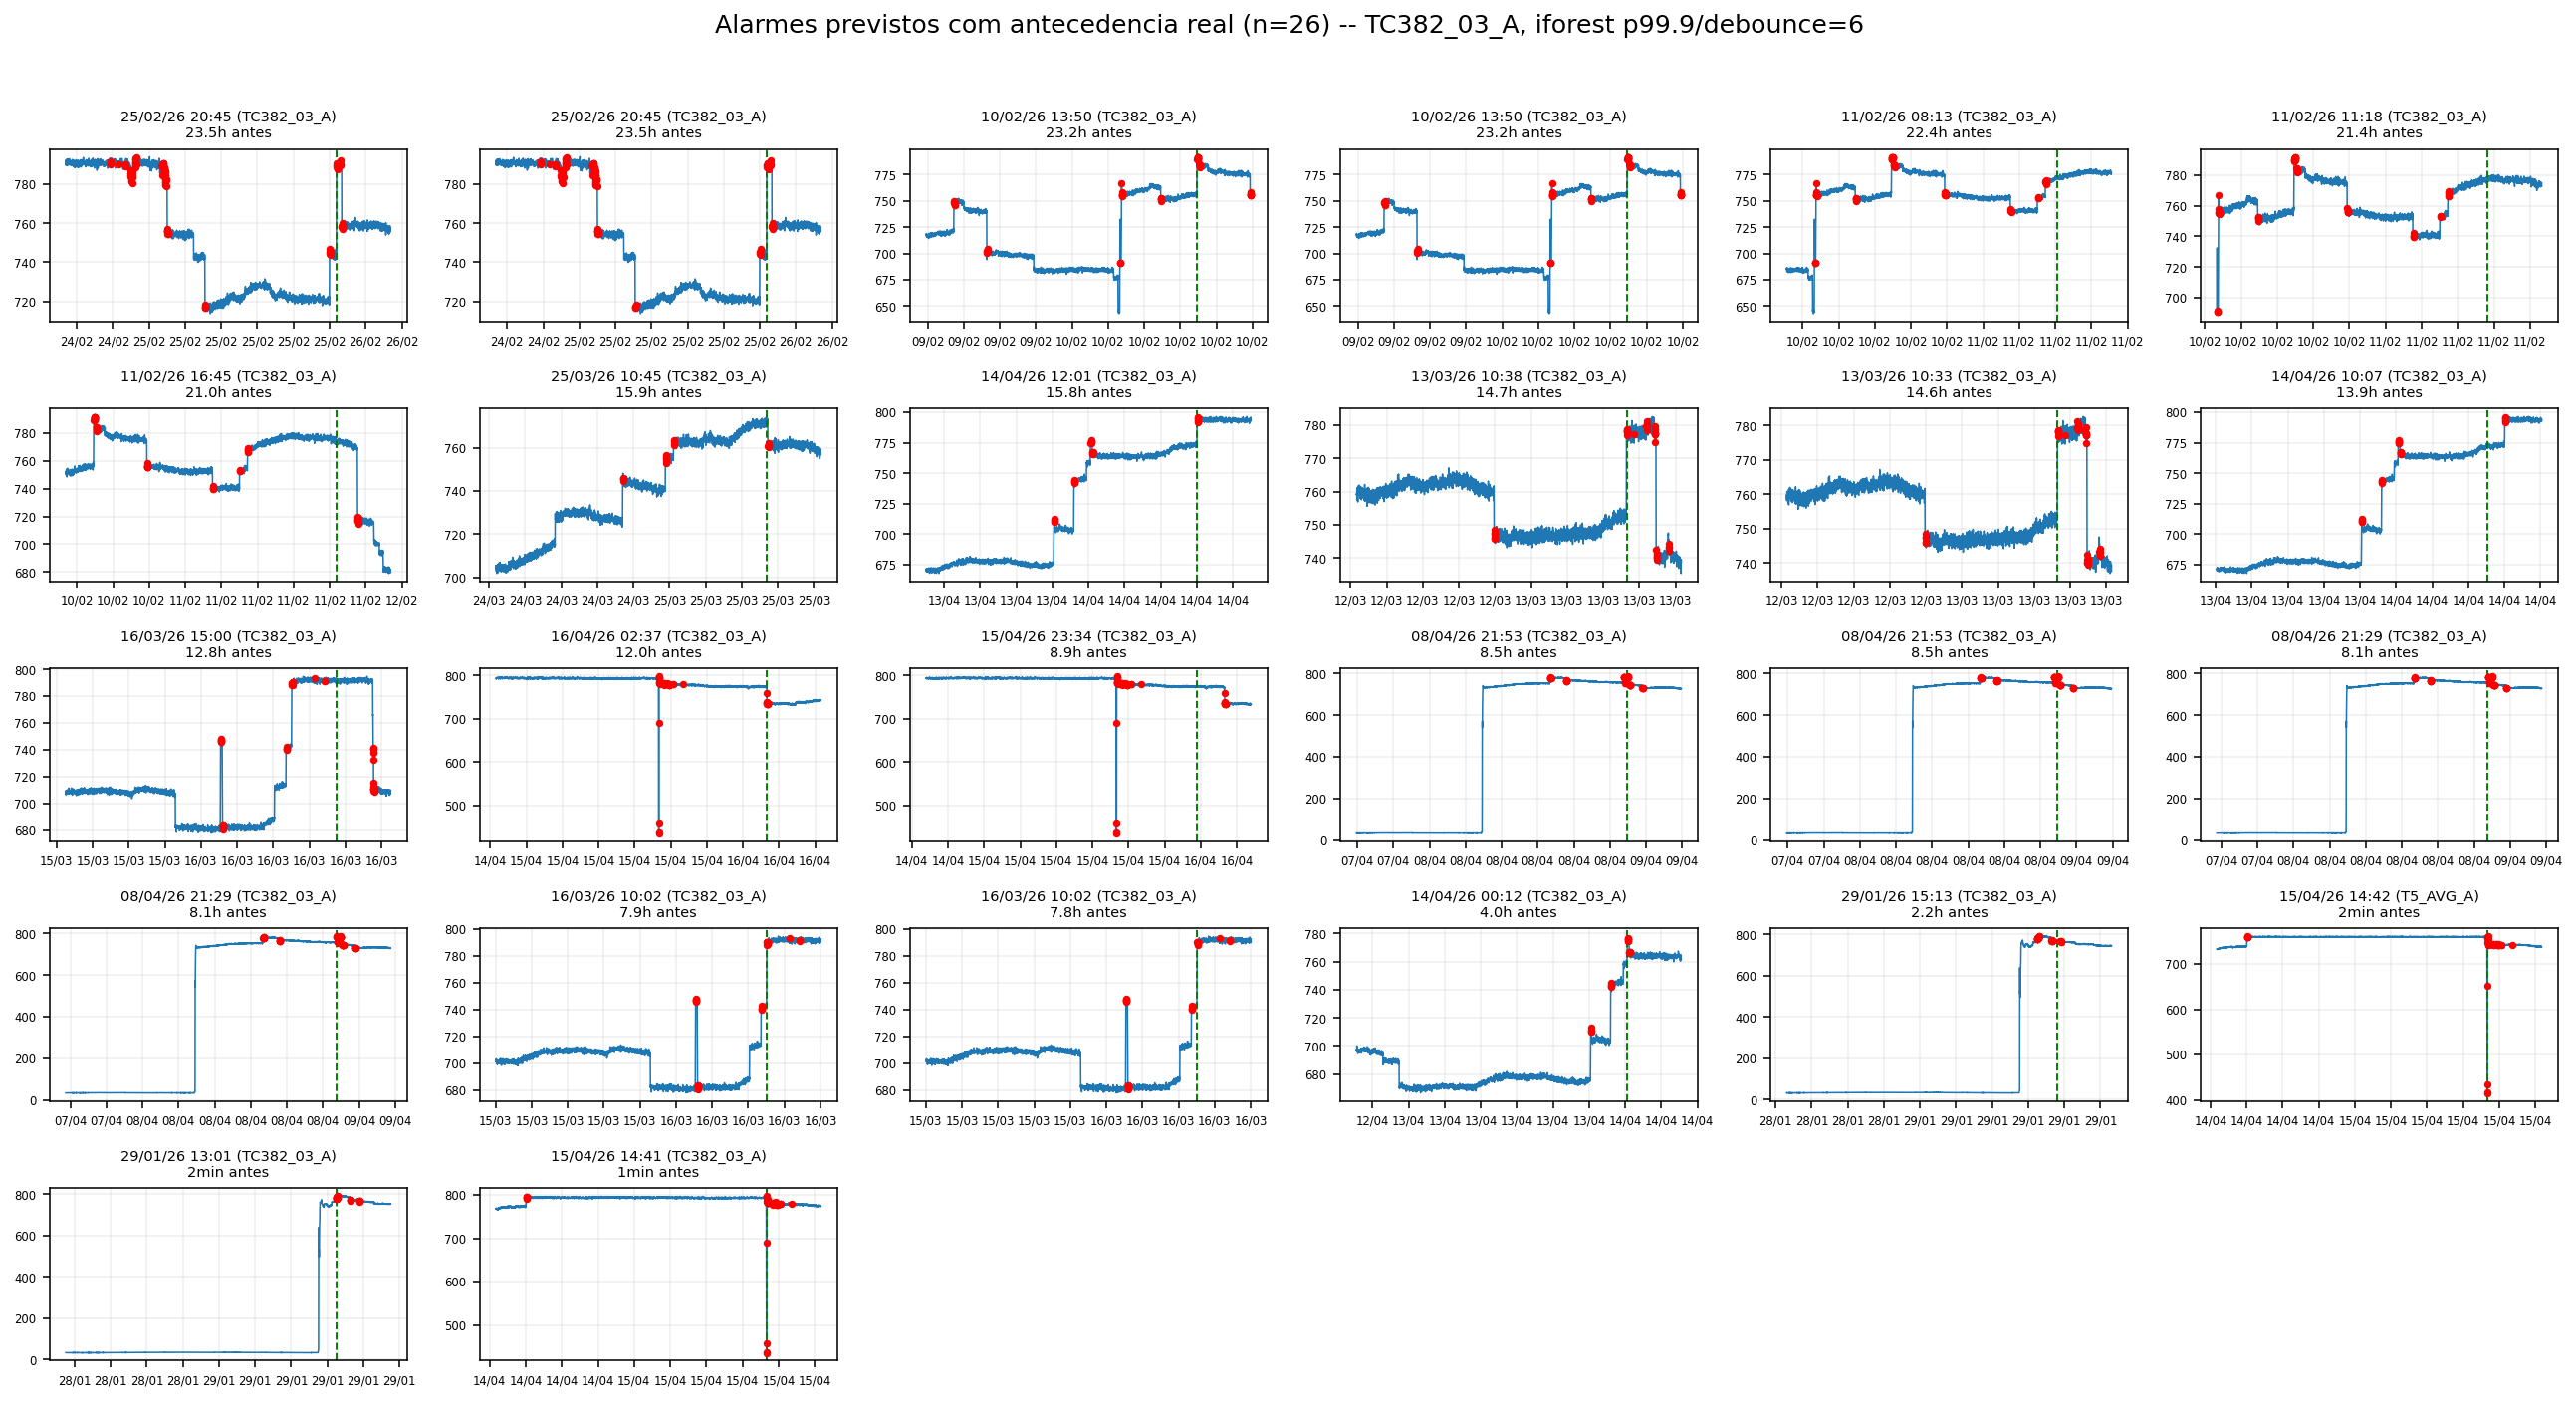
\includegraphics[width=\textwidth]{figs/exp6/04_painel_preditivos.png}
\caption{Os 26 casos com antecedência real, da maior para a menor
antecedência. Vários mostram um padrão em ``escada'' -- quedas ou subidas
sucessivas de temperatura, já sinalizadas como anomalia horas antes do
alarme.}
\end{figure}

\begin{figure}[H]
\centering
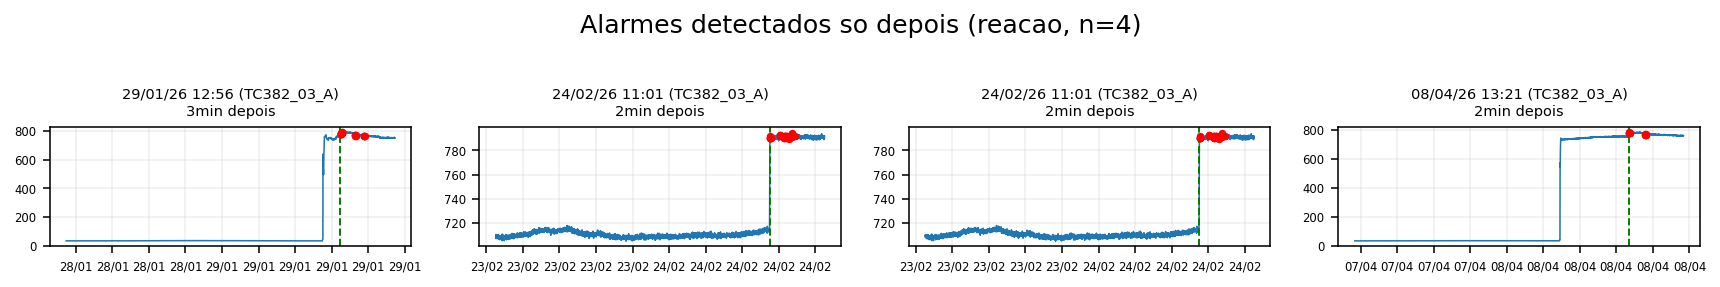
\includegraphics[width=0.7\textwidth]{figs/exp6/05_painel_reativos.png}
\caption{Os 4 casos em que a detecção só veio depois do alarme.}
\end{figure}

\begin{figure}[H]
\centering
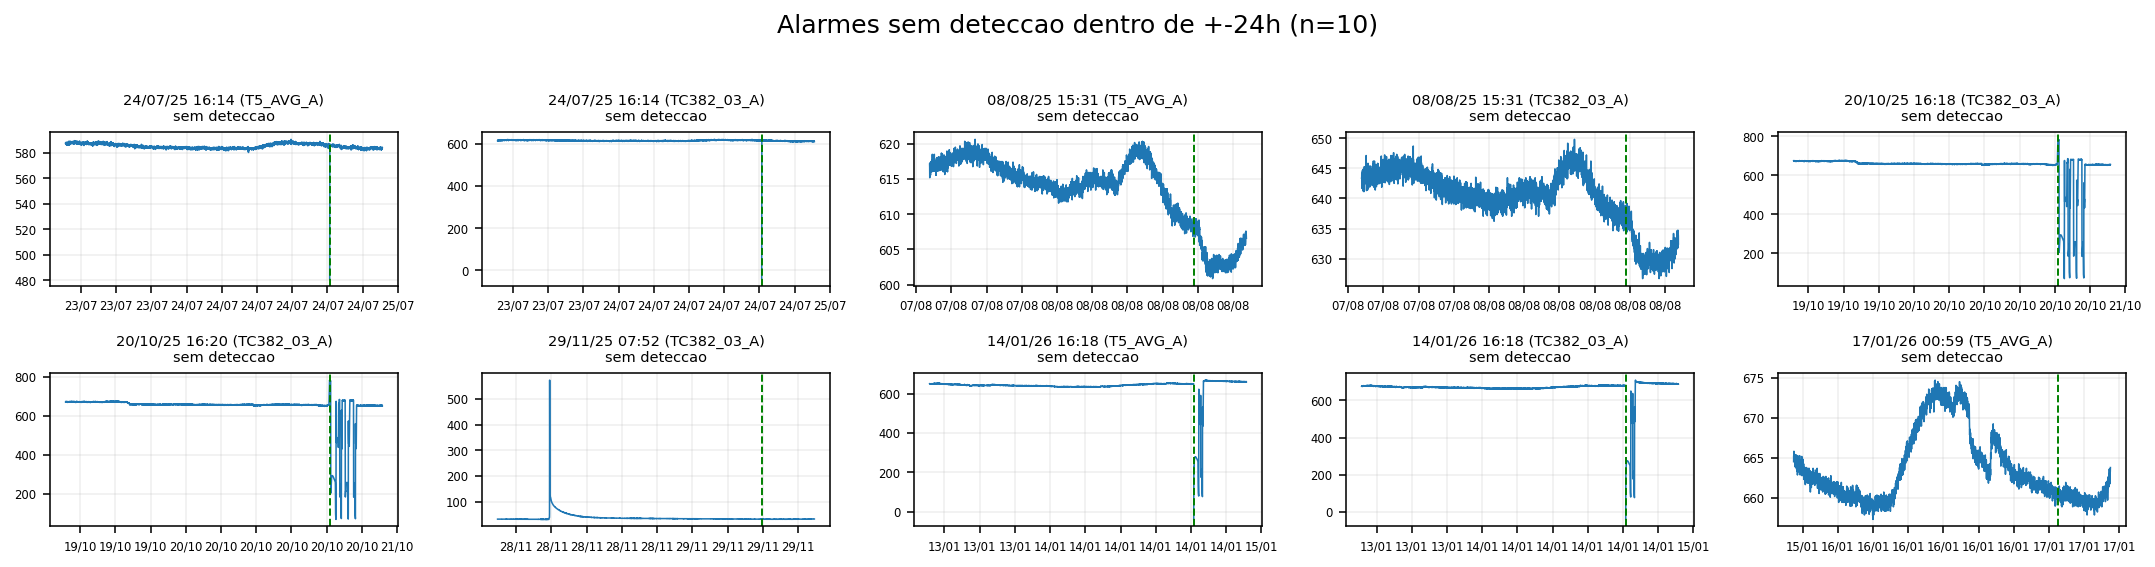
\includegraphics[width=\textwidth]{figs/exp6/06_painel_perdidos.png}
\caption{Os 10 alarmes sem nenhuma detecção em $\pm$24h -- a maioria não
mostra excursão visível na própria série de temperatura plotada. Estes 10
casos, junto com os 4 reativos acima, são exatamente o alvo do EXP7
(Parte~\ref{part:exp7}).}
\label{fig:exp6-perdidos}
\end{figure}

\textbf{Dois pontos fracos claros ao final do EXP6:} 4 alarmes detectados
só depois do fato (reação, não previsão) e 10 sem detecção alguma dentro
de $\pm$24h. É exatamente daqui que o EXP7 parte.

\clearpage
% =====================================================================
\part{EXP7: fechando os pontos fracos do EXP6}
\label{part:exp7}
% =====================================================================

% ---------------------------------------------------------------------
\section{Visão geral e plano de ataque}
% ---------------------------------------------------------------------

Antes de qualquer mudança de código, investigamos o estado da arte em
manutenção preditiva especificamente para os dois problemas do EXP6 --
falta de antecedência (reativo) e ausência total de sinal (sem detecção).
Cinco direções foram priorizadas, da mais barata/baixo-risco à mais
custosa:

\begin{enumerate}
  \item \textbf{Features multi-escala} -- as features do EXP6 só olham uma
        janela de 6 min, curta demais para um precursor que se desenvolve
        ao longo de horas.
  \item \textbf{Features de textura do sinal} -- kurtosis, skewness, crest
        factor capturam mudança de \emph{forma} do sinal de vibração, não
        só nível ou tendência.
  \item \textbf{Detecção de mudança de regime} (CUSUM/z-score de linha de
        base local) -- complementar ao threshold por percentil global,
        que pode ser cego a um drift lento que nunca fica ``extremo''.
  \item \textbf{Reformulação supervisionada} -- treinar direto ``vai
        alarmar nas próximas N horas?'' usando os alarmes como rótulo.
  \item \textbf{RUL/sobrevivência} -- aspiracional, requer mais eventos
        rotulados.
\end{enumerate}

Este relatório cobre os itens 1--3 (a linha de raciocínio contínua de
engenharia de features sobre o mesmo modelo não supervisionado). Os itens
4--5 foram tentados à parte (classificador supervisionado: resultado
negativo, dominado pelo AutoML em todo o grid testado; sobrevivência
exploratória: achado de hazard decrescente/rajadas de alarme, mas não é
modelo operacional) e não alteraram o candidato de referência --
documentados em \texttt{docs/analise\_automl\_exp8.md}.

Mesma base de dados, mesmo grupo de sensores, mesma janela temporal do
EXP6 em todos os itens a seguir -- muda exclusivamente a engenharia de
features.

% ---------------------------------------------------------------------
\section{Item 1 --- Features multi-escala}
\label{sec:item1}
% ---------------------------------------------------------------------

\subsection{Onde paramos}

Ao final do EXP6 (Seção~\ref{sec:resultado-exp6}): 26 preditivos, 4
reativos, \textbf{10 sem detecção} (Figura~\ref{fig:exp6-perdidos}).
Hipótese de causa raiz: a única janela de 6 min é cega a um precursor que
se desenvolve em escala de horas -- a tendência lenta nunca gera um
\texttt{delta\_1} grande o suficiente, e o valor em si pode nunca cruzar o
percentil global mesmo já tendo saído da linha de base recente daquele
trecho.

\subsection{O que muda: quatro janelas em vez de uma}

Antes (EXP6): uma única janela de 12 amostras (6 min). Agora
(\texttt{DERIVED\_ROLLING\_WINDOWS=[12, 120, 480, 2880]}): quatro janelas
simultâneas -- 6 min, 1h, 4h e 24h. Para cada sensor e cada janela: média
móvel, desvio móvel e \texttt{trend\_w} (valor atual menos o valor de
\texttt{w} passos atrás). $48 \to 168$ features de entrada.

\begin{figure}[H]
\centering
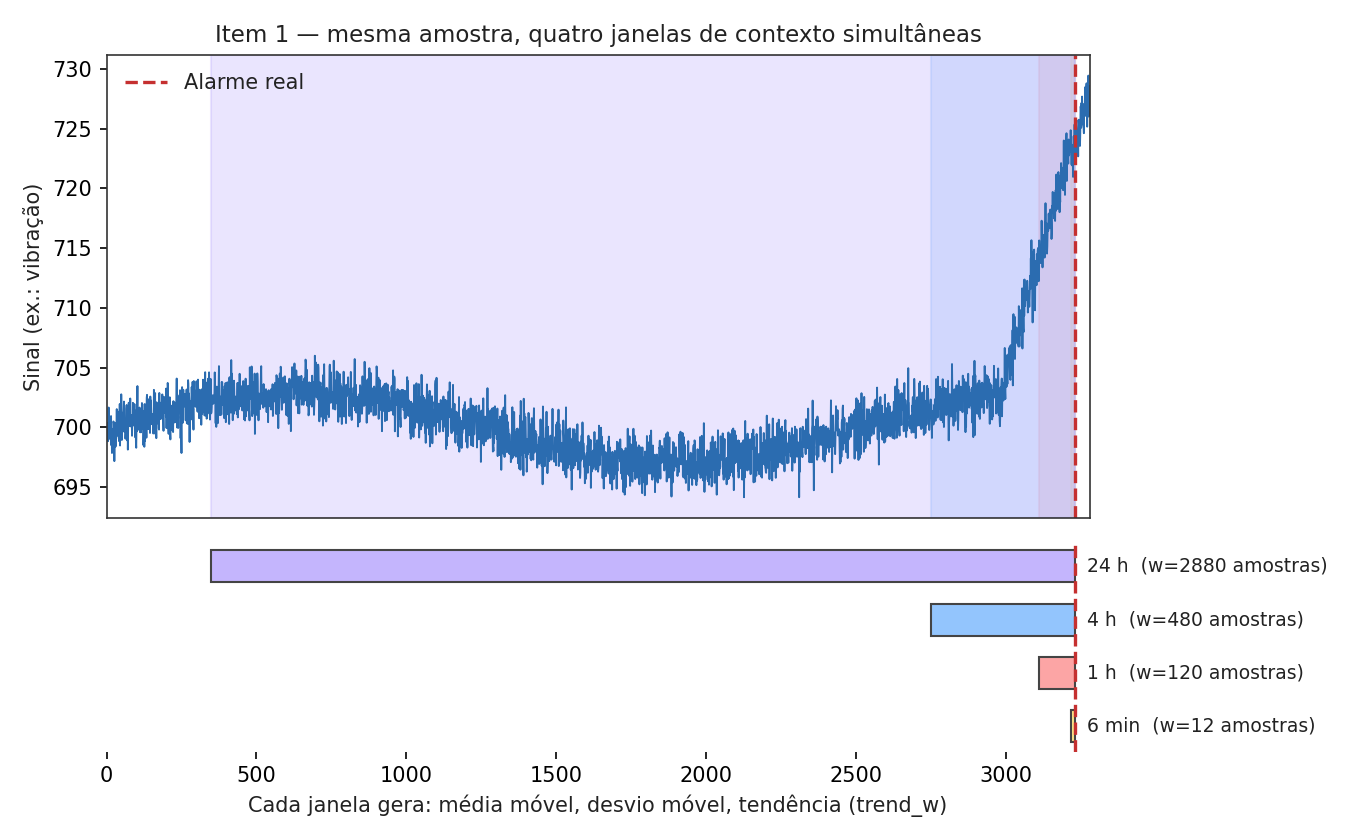
\includegraphics[width=0.92\textwidth]{figs/schema_item1_multiescala.png}
\caption{Esquema do mecanismo: a mesma amostra no tempo (linha vertical
tracejada = alarme) passa a ter contexto de 4 escalas diferentes ao mesmo
tempo. A janela de 6 min captura só a inclinação final abrupta; as janelas
de 4h/24h enxergam o platô e o início da subida lenta que a janela curta
não via.}
\end{figure}

\subsection{Configuração de treinamento}

Idêntica ao EXP6 (Seção~\ref{sec:dados-exp6}), exceto
\texttt{DERIVED\_ROLLING\_WINDOWS=[12, 120, 480, 2880]} no lugar da janela
única -- sem mudança em máscaras, split OOS, grid de threshold/debounce ou
\texttt{eval\_sensors}.

\subsection{Resultado: mais cobertura, mais falso alerta}

\begin{table}[H]
\centering
\begin{tabular}{@{}lcc@{}}
\toprule
\textbf{Métrica} & \textbf{EXP6 (janela única)} & \textbf{Item 1 (multi-escala)} \\
\midrule
Melhor modelo & iforest p99,9/db6 & ocsvm p99,5/db6 \\
hit\_rate & 75,0\% (30/40) & \textbf{87,5\% (35/40)} \\
\textbf{Preditivo} & 26 & \textbf{28} \\
Reativo & 4 & 7 \\
\textbf{Sem detecção} & \textbf{10} & \textbf{5} \\
FP (normal\_alert\_rate) & 0,06\% & 2,21\% \\
Mediana de antecedência & 12,4h & \textbf{15,0h} \\
\bottomrule
\end{tabular}
\caption{Ganho: sem detecção cai pela metade (10$\to$5), antecedência
mediana melhora. Perda: falso alerta $\sim$37$\times$ maior -- uma troca
real, não um upgrade de graça.}
\end{table}

\begin{figure}[H]
\centering
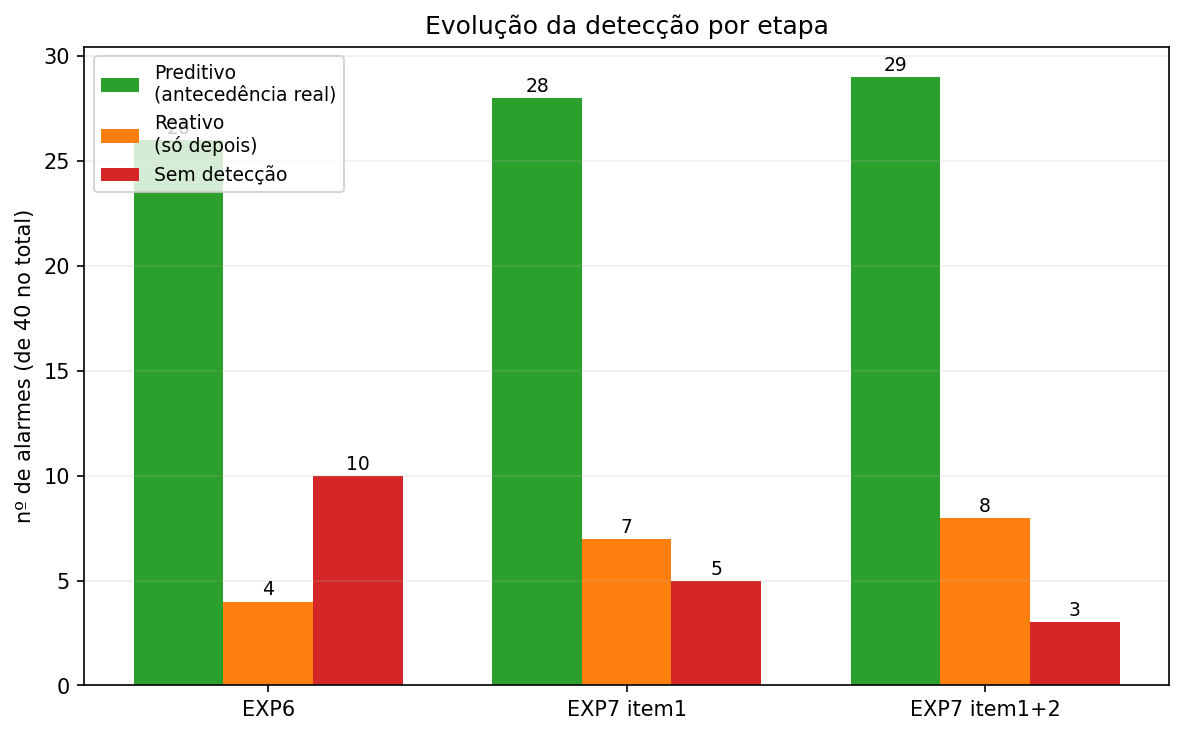
\includegraphics[width=0.85\textwidth]{figs/exp7/01_evolucao_categorias.png}
\caption{Evolução do número de alarmes em cada categoria -- esta figura
acompanha as três etapas do EXP7 (item 1, item 1+2, e o item 1+2+3 da
Seção~\ref{sec:item3}) e será referenciada de novo adiante. Sem detecção
cai de 10 para 3 ao longo da série; preditivo sobe de 26 para 29.}
\label{fig:evolucao-categorias}
\end{figure}

\begin{figure}[H]
\centering
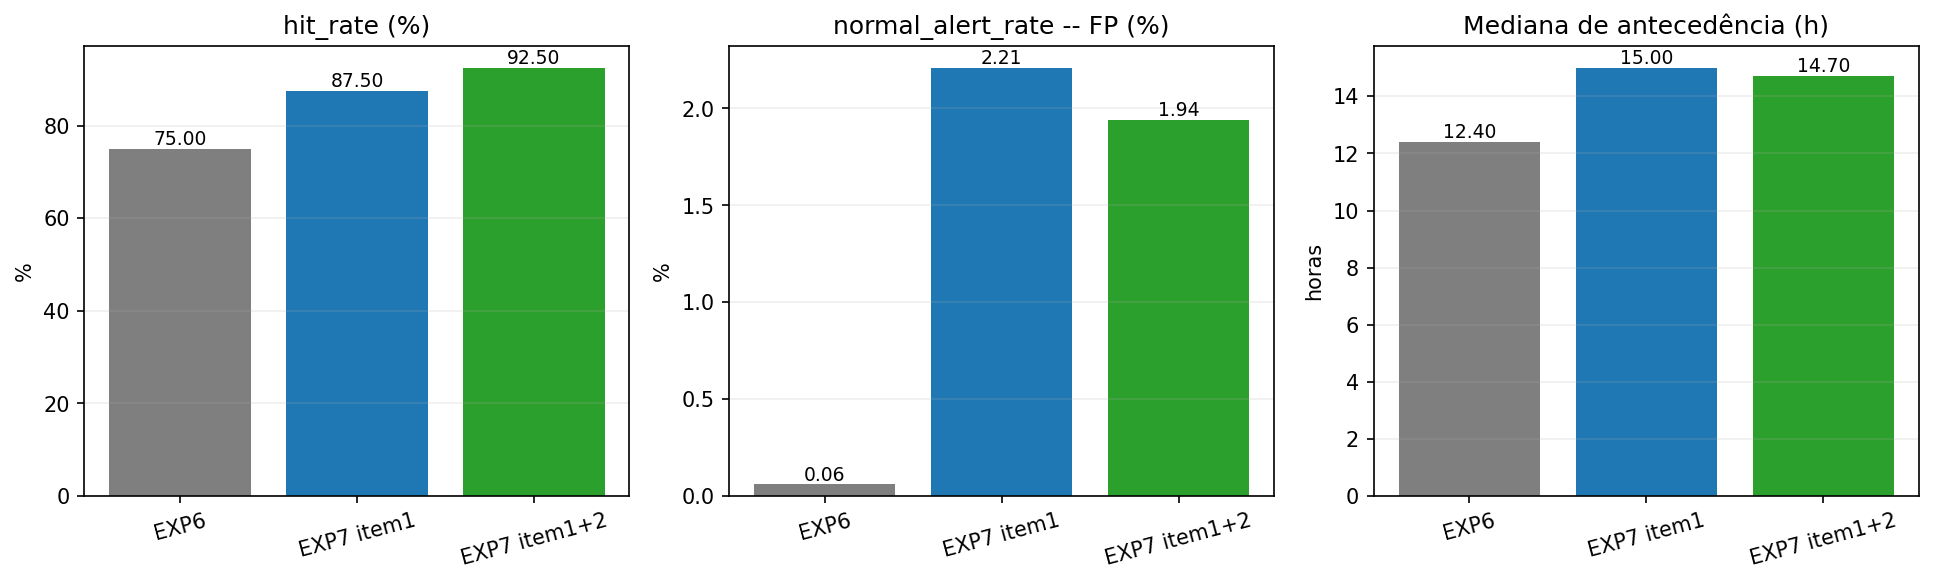
\includegraphics[width=\textwidth]{figs/exp7/02_metricas_por_etapa.png}
\caption{hit\_rate, falso alerta e mediana de antecedência por etapa --
gráfico de referência para acompanhar a diminuição/aumento de falso alerta
ao longo de toda a série EXP6$\to$EXP7. Note que o FP do EXP6 (0,06\%) é
proporcionalmente muito menor que os do EXP7 -- a troca de cobertura por
falso alerta é real e está sendo mostrada, não escondida.}
\end{figure}

\subsection{Desvio: o candidato de baixo FP que parecia bom mas não era}
\label{sec:licao}

No mesmo grid multi-escala, o melhor trial de \texttt{iforest} com FP
mínimo e hit\_rate$\geq$70\% (p99,0/debounce=12: 70\% hit / 0,38\% FP)
parecia, pelos números agregados, uma alternativa mais conservadora.
Isolamos esse trial numa run dedicada para abrir o detalhamento:

\begin{table}[H]
\centering
\begin{tabular}{@{}lccc@{}}
\toprule
\textbf{Candidato} & \textbf{hit\_rate / FP} & \textbf{Preditivo} & \textbf{Reativo} \\
\midrule
ocsvm multi-escala (escolhido) & 87,5\% / 2,21\% & \textbf{28} & 7 \\
iforest ``baixo FP'' (mesma etapa) & 70,0\% / 0,38\% & \textbf{13} & 15 \\
\bottomrule
\end{tabular}
\caption{Apesar do FP baixo, esse candidato é o \textbf{pior em
antecedência real} -- só 13 das 28 detecções são preditivas, o resto é
reação tardia (\texttt{debounce=12}, o dobro do padrão, atrasa o ponto que
``conta'' como detecção).}
\end{table}

\textbf{Lição:} \texttt{hit\_rate}/\texttt{normal\_alert\_rate} agregados
enganam -- é preciso sempre abrir o detalhamento preditivo/reativo/sem
detecção antes de escolher um candidato pelo score agregado. Esta é a
mesma disciplina que será aplicada de novo no EXP10 (fragmentação em
episódios em vez de confiar em taxas agregadas).

\textbf{Candidato de referência após o item 1:} \texttt{ocsvm} multi-escala
(p99,5/db6).

% ---------------------------------------------------------------------
\section{Item 2 --- Textura do sinal (kurtosis, skewness, crest factor)}
\label{sec:item2}
% ---------------------------------------------------------------------

\subsection{Onde paramos}

Ao final do item 1: 28 preditivos, 7 reativos, 5 sem detecção, FP de
2,21\%. O ganho de cobertura veio a um custo real de falso alerta -- o
item 2 testa se dá para melhorar cobertura \emph{sem} pagar mais esse
preço.

\subsection{O que muda: forma do sinal, não só nível}

Para as janelas $\geq$1h (a de 6 min não tem amostra suficiente para esses
estimadores serem estáveis), três features adicionais por sensor:
kurtosis móvel, skewness móvel e crest factor móvel (pico $\div$ RMS
dentro da janela). $168 \to 276$ features de entrada.

\begin{figure}[H]
\centering
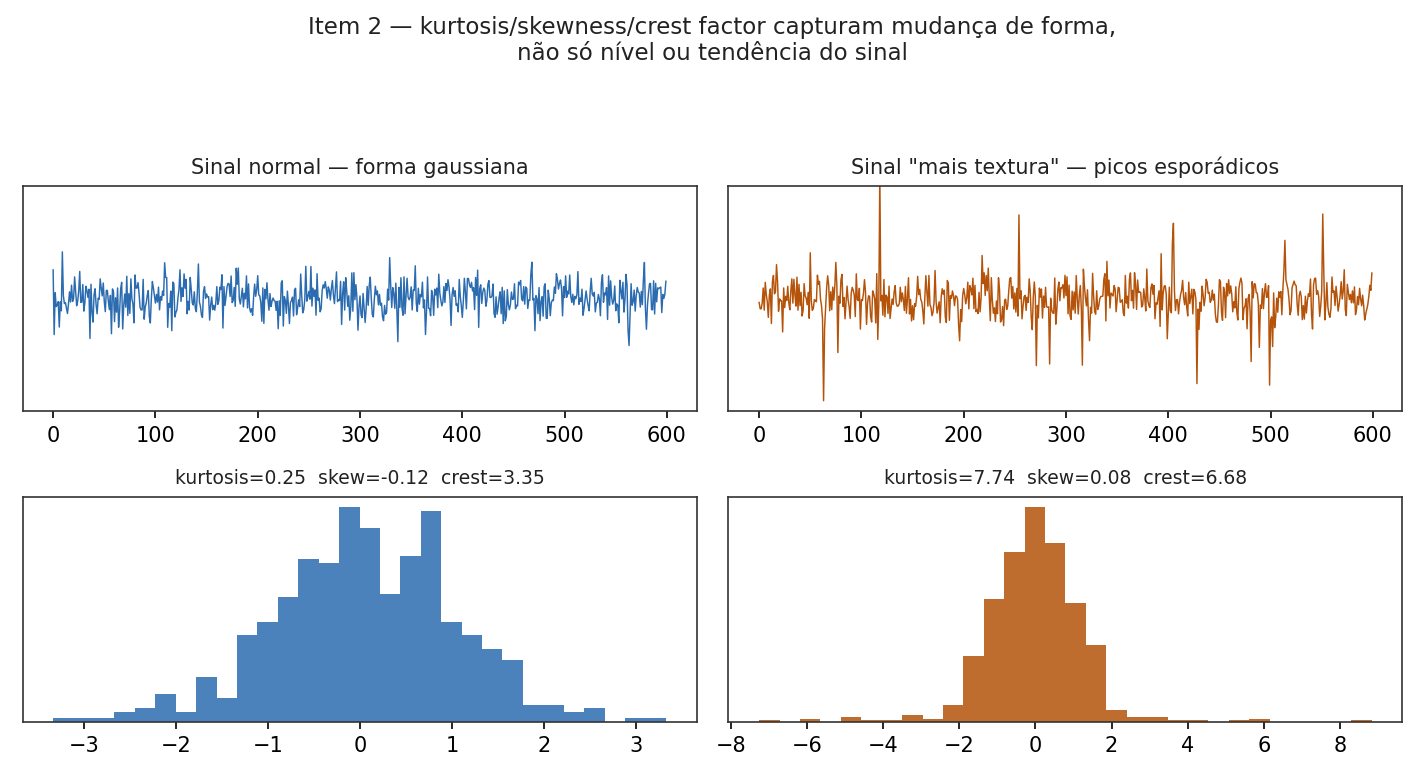
\includegraphics[width=0.92\textwidth]{figs/schema_item2_textura.png}
\caption{Esquema do mecanismo: dois sinais com a mesma média e desvio
padrão aproximados podem ter kurtosis/skewness/crest factor muito
diferentes. O sinal ``com textura'' (direita) tem picos esporádicos --
kurtosis $7{,}7$ vs $0{,}25$ do sinal normal -- que média/desvio sozinhos
não capturam, mas que são o padrão de degradação incipiente de mancal em
condition monitoring.}
\end{figure}

\subsection{Configuração de treinamento}

Idêntica ao item 1, com a adição das 3 features de textura por sensor nas
janelas de 1h/4h/24h -- sem mudança em máscaras, split OOS, grid ou
\texttt{eval\_sensors}.

\subsection{Resultado: ganho limpo em todos os eixos ao mesmo tempo}

\begin{table}[H]
\centering
\begin{tabular}{@{}lcc@{}}
\toprule
\textbf{Métrica} & \textbf{Item 1 (multi-escala)} & \textbf{Item 1+2 (+ textura)} \\
\midrule
Melhor modelo & ocsvm p99,5/db6 & ocsvm p99,9/db1 \\
hit\_rate & 87,5\% (35/40) & \textbf{92,5\% (37/40)} \\
\textbf{Preditivo} & 28 & \textbf{29} \\
Reativo & 7 & 8 \\
\textbf{Sem detecção} & 5 & \textbf{3} \\
FP (normal\_alert\_rate) & 2,21\% & \textbf{1,94\%} \\
Mediana de antecedência & 15,0h & 14,7h \\
\bottomrule
\end{tabular}
\caption{Ao contrário do item 1 (trocou FP por cobertura), o item 2
melhora hit\_rate, FP \emph{e} a divisão preditivo/sem-detecção ao mesmo
tempo -- indício de que kurtosis/skewness/crest factor capturam sinal
genuíno de vibração ficando ``mais irregular'' antes do evento, não só
reclassificam detecções reativas ao acaso.}
\end{table}

Já mostrado na Figura~\ref{fig:evolucao-categorias}: sem detecção cai de
10 (EXP6) para 5 (item 1) para 3 (item 1+2) -- a curva de melhoria
contínua ao longo dos testes, sem retrocesso em nenhuma etapa.

\subsection{Gráficos do que acertamos e do que não acertamos}

Candidato final desta etapa: \texttt{ocsvm} (percentil 99,9, debounce=1)
sobre o grupo com 276 features de entrada. As Figuras
\ref{fig:pred-item2}--\ref{fig:miss-item2} mostram \textbf{todos os 40
alarmes} da avaliação, agrupados por categoria -- o sensor-alvo plotado em
cada miniatura é o mesmo que gerou aquele alarme específico.

\begin{figure}[H]
\centering
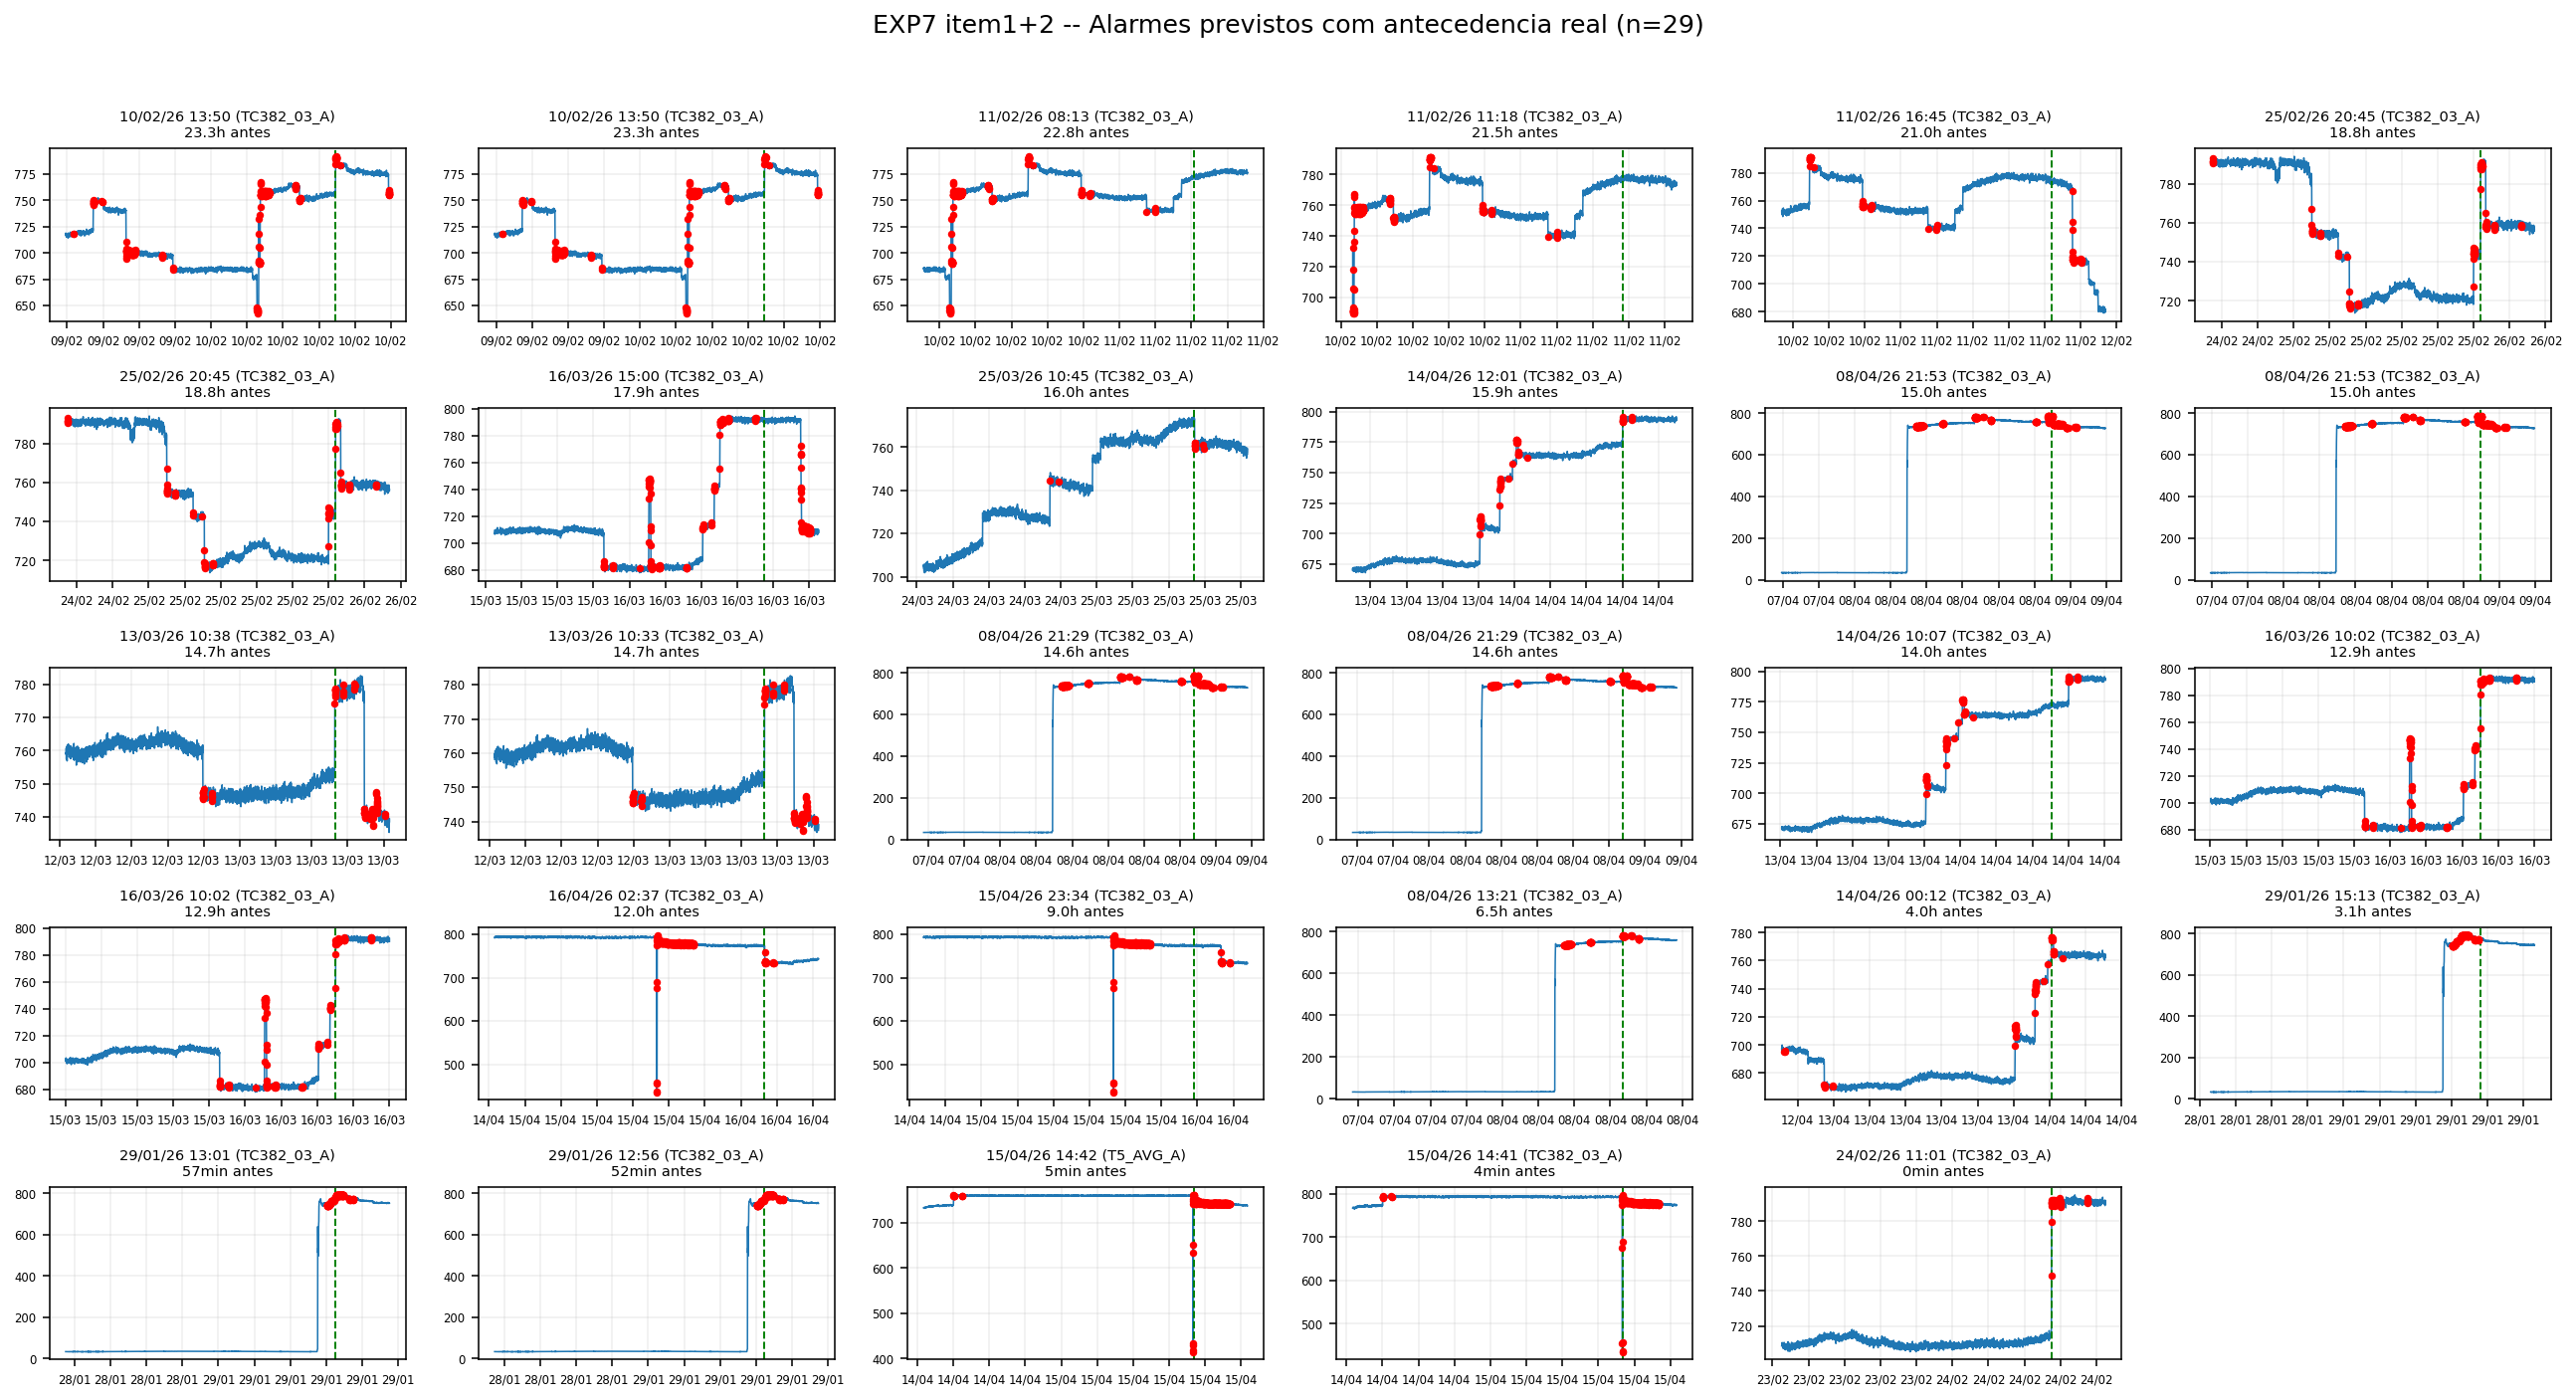
\includegraphics[width=\textwidth]{figs/exp7/03_painel_preditivos.png}
\caption{Os 29 casos com antecedência real, da maior (23,3h) para a menor
antecedência (poucos segundos). Mediana de 14,7h.}
\label{fig:pred-item2}
\end{figure}

\begin{figure}[H]
\centering
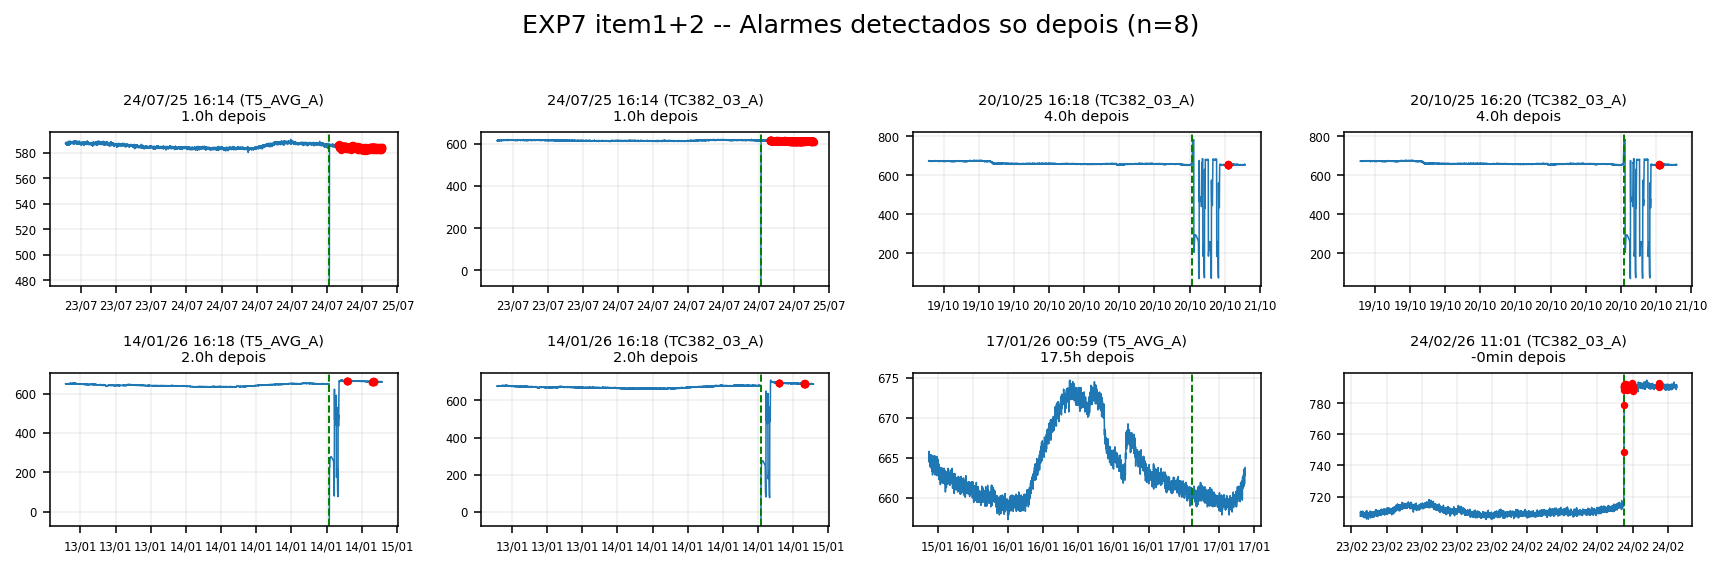
\includegraphics[width=0.85\textwidth]{figs/exp7/04_painel_reativos.png}
\caption{Os 8 casos em que a detecção só veio depois (ou praticamente
junto) do alarme.}
\end{figure}

\begin{figure}[H]
\centering
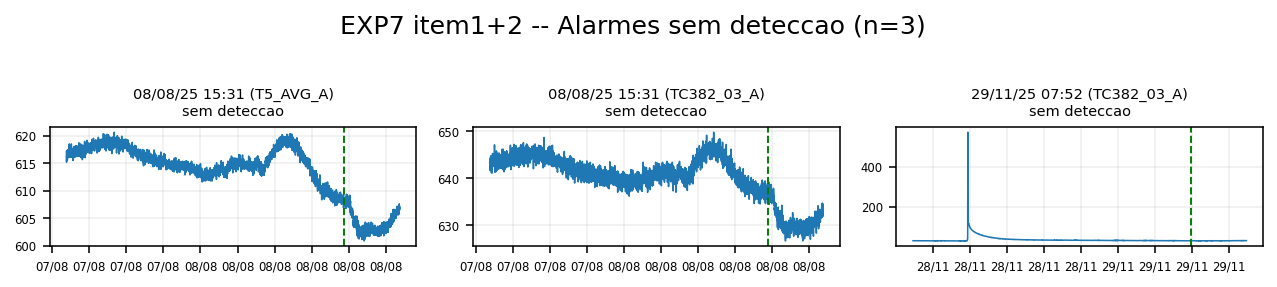
\includegraphics[width=0.75\textwidth]{figs/exp7/05_painel_perdidos.png}
\caption{Os 3 alarmes restantes sem detecção -- caíram de 10 (EXP6) para
3. Investigados em detalhe na Seção~\ref{sec:qualidade}.}
\label{fig:miss-item2}
\end{figure}

\textbf{Candidato de referência após o item 2 (inalterado até o EXP10):}
\texttt{ocsvm} (p99,9/debounce=1) sobre \texttt{TC382\_T5\_vibracao\_mancais}
com features multi-escala + textura.

% ---------------------------------------------------------------------
\section{Item 3 --- Detecção de mudança de regime (CUSUM + z-score local)}
\label{sec:item3}
% ---------------------------------------------------------------------

\subsection{Onde paramos}

Ao final do item 2: 29 preditivos, 8 reativos, \textbf{3 sem detecção}.
Restam 3 casos sem nenhum sinal em $\pm$24h -- o item 3 foi escolhido
especificamente para atacar esses residuais: em vez de exigir que o valor
cruze um limiar histórico fixo, detectar quando o trecho já é
estatisticamente diferente da sua \emph{linha de base local} recente.

\subsection{O que muda: linha de base local em vez de limiar global}

Duas features causais novas por sensor: \texttt{localz\_\{1h\}\_\{24h\}}
(z-score da média de curto prazo em relação à linha de base de 24h) e
\texttt{cusum\_pos}/\texttt{cusum\_neg} (CUSUM causal de Page, acumula
evidência de desvio sustentado da média móvel de 24h, com folga de 0,5
desvio-padrão local). $276 \to 312$ features de entrada.

\begin{figure}[H]
\centering
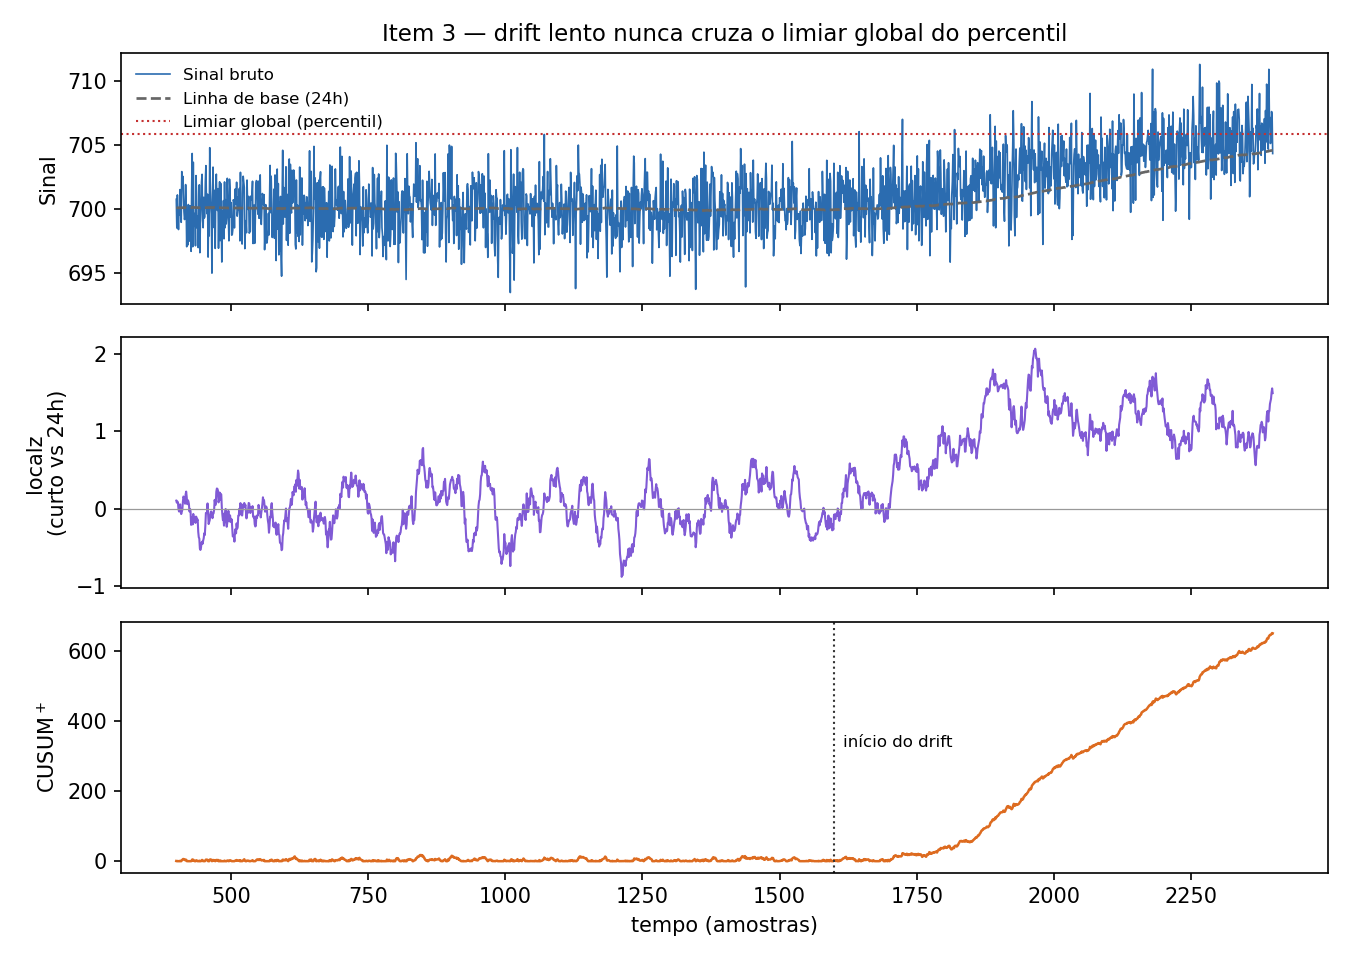
\includegraphics[width=0.92\textwidth]{figs/schema_item3_cusum.png}
\caption{Esquema do mecanismo: um drift lento (painel superior) nunca
cruza o limiar global do percentil (linha vermelha pontilhada) porque a
linha de base (tracejada cinza) sobe junto -- mas tanto o z-score local
(painel do meio) quanto o CUSUM (painel inferior) acumulam evidência do
desvio sustentado, mesmo sem nenhum valor ``extremo'' isolado.}
\end{figure}

\subsection{Configuração de treinamento}

Idêntica ao item 1+2, com a adição das 2 features de mudança de regime por
sensor -- sem mudança em máscaras, split OOS, grid ou \texttt{eval\_sensors}.

\subsection{Resultado: nenhum ganho adicional}

\begin{table}[H]
\centering
\begin{tabular}{@{}lcc@{}}
\toprule
\textbf{Métrica} & \textbf{Item 1+2 (textura)} & \textbf{Item 1+2+3 (+ regime)} \\
\midrule
hit\_rate & 92,5\% & 92,5\% \\
FP & 1,94\% & 1,93\% \\
Preditivo & 29 & 29 \\
Reativo & 8 & 8 \\
Sem detecção & \textbf{3} & \textbf{3 (os mesmos 3 casos)} \\
Mediana de antecedência & 14,7h & 14,7h (idêntico) \\
\bottomrule
\end{tabular}
\caption{Os números batem exatamente -- o \texttt{threshold} do
\texttt{ocsvm} vencedor mudou de 14,88 para 16,07 (as novas features
entraram no ajuste do modelo), mas isso não mudou a classificação final
nos 3 casos residuais.}
\end{table}

\begin{figure}[H]
\centering
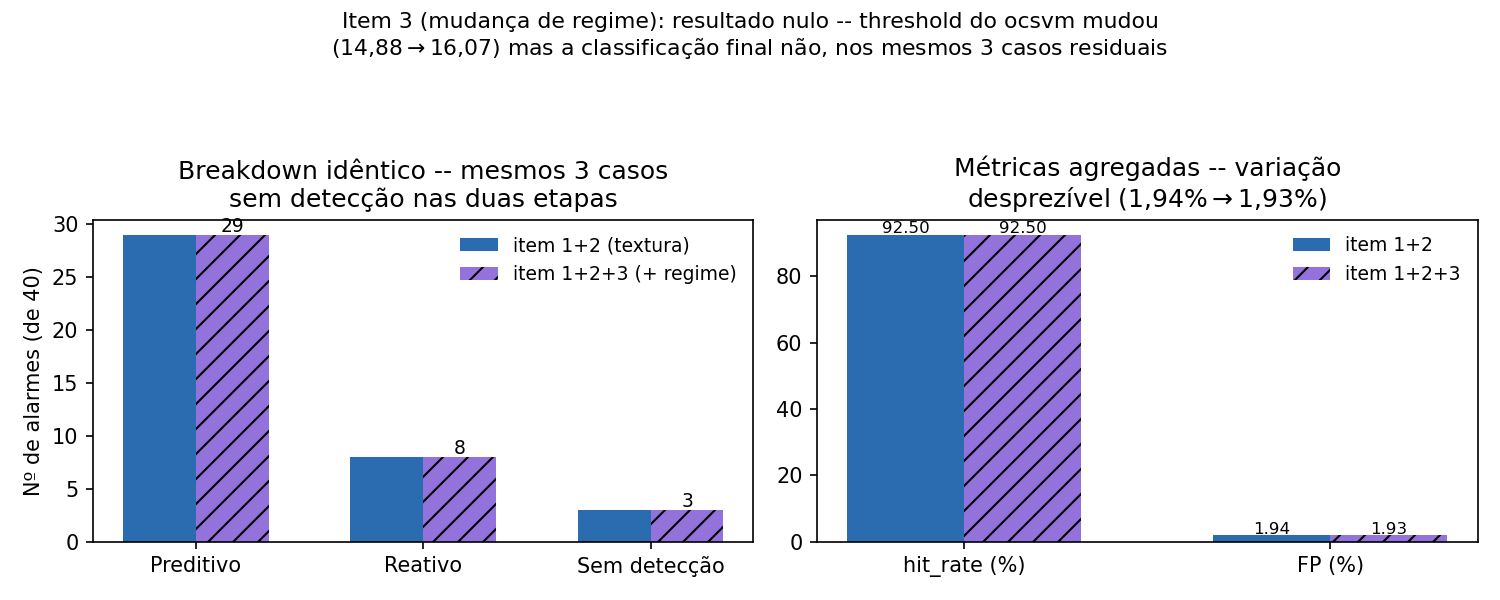
\includegraphics[width=0.92\textwidth]{figs/item3_resultado_nulo.png}
\caption{Resultado nulo do item 3: breakdown preditivo/reativo/sem
detecção idêntico, e variação de FP/hit\_rate desprezível.}
\end{figure}

\textbf{Interpretação:} os 3 alarmes residuais provavelmente não têm
nenhum precursor detectável nos sensores disponíveis (temperatura +
vibração) -- nem em nível, nem em tendência, nem em mudança de regime
local. É possível que tenham causa externa ao que monitoramos (ação de
operador, trip por outro sistema) que não deixa rastro nesses canais
especificamente. \textbf{Não vale insistir nessa direção com os dados
atuais} -- confirmado com mais detalhe na investigação caso a caso da
Seção~\ref{sec:reativos}.

% ---------------------------------------------------------------------
\section{Aprofundamento: qualidade dos alarmes}
\label{sec:qualidade}
% ---------------------------------------------------------------------

Depois de fechar os itens 1--3, investigamos os 40 alarmes da avaliação
OOS um a um: de qual sensor, em qual condição, e -- o ponto central desta
seção -- \textbf{quais são eventos físicos reais e quais são artefato de
falha de sensor/comunicação}.

\subsection{Os 40 alarmes não são homogêneos}

\begin{table}[H]
\centering
\begin{tabular}{@{}lcc@{}}
\toprule
\textbf{Sensor} & \textbf{Alarmes} & \textbf{\%} \\
\midrule
TC382\_03\_A & 35 & 87,5\% \\
T5\_AVG\_A & 5 & 12,5\% \\
\bottomrule
\end{tabular}
\qquad
\begin{tabular}{@{}lc@{}}
\toprule
\textbf{Condição} & \textbf{Qtd.} \\
\midrule
HI & 18 \\
HIHI & 14 \\
UNDER & 8 \\
\bottomrule
\end{tabular}
\end{table}

\begin{table}[H]
\centering
\begin{tabular}{@{}lcccc@{}}
\toprule
\textbf{Condição} & \textbf{Preditivo} & \textbf{Reativo} & \textbf{Sem detecção} & \textbf{Taxa preditiva} \\
\midrule
HI & 16 & 2 & 0 & 88,9\% \\
HIHI & 13 & 1 & 0 & 92,9\% \\
\textbf{UNDER} & \textbf{0} & 5 & 3 & \textbf{0\%} \\
\bottomrule
\end{tabular}
\caption{Antecedência quase perfeita para HI/HIHI; \textbf{zero}
antecedência para UNDER.}
\end{table}

\begin{figure}[H]
\centering
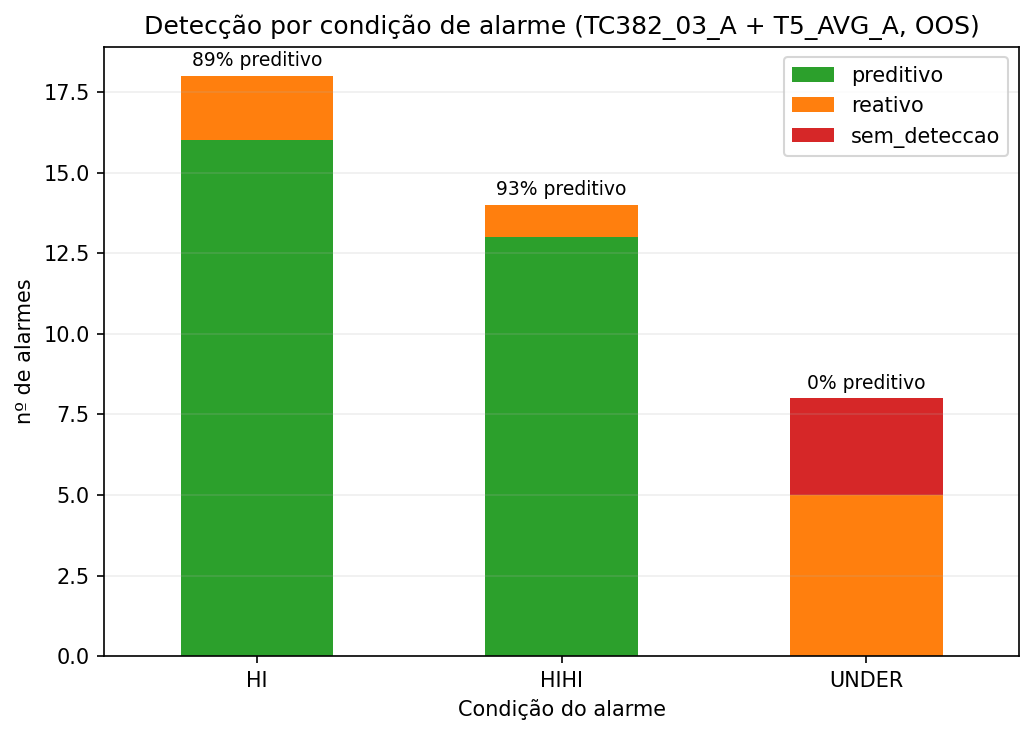
\includegraphics[width=0.75\textwidth]{figs/exp7q/01_deteccao_por_condicao.png}
\caption{Detecção por condição de alarme.}
\end{figure}

\subsection{UNDER é falha de sensor, não evento físico}

Os 8 alarmes \texttt{UNDER} disparam com valor entre $-18$ e $-22$ --
fisicamente implausível (operação normal $\sim$600--800, mesmo em
idle/frio $\sim$25--40). Verificação direta na série bruta, para cada um
dos 5 instantes distintos:

\begin{table}[H]
\centering
\small
\begin{tabular}{@{}lp{9cm}@{}}
\toprule
\textbf{Alarme} & \textbf{Evidência} \\
\midrule
08/08/2025 15:31 & 9 de 12 pontos NaN em \texttt{TC382\_03\_A}; \texttt{RUNNING\_A=1} o tempo todo -- gap de dado. \\
17/01/2026 00:59 & \texttt{RUNNING\_A}=\texttt{Comm Fail}/\texttt{Out of Serv} -- falha de comunicação explícita. \\
29/11/2025 07:52 & \texttt{RUNNING\_A=0} -- equipamento já desligado. \\
24/07/2025 16:14 & Transição \texttt{RUNNING\_A} 1$\to$0 -- parada em andamento. \\
14/01/2026 16:18 & Mistura de \texttt{Out of Serv}/transição. \\
\bottomrule
\end{tabular}
\caption{Nenhum dos 5 casos é queda física real de temperatura em operação normal.}
\end{table}

\begin{figure}[H]
\centering
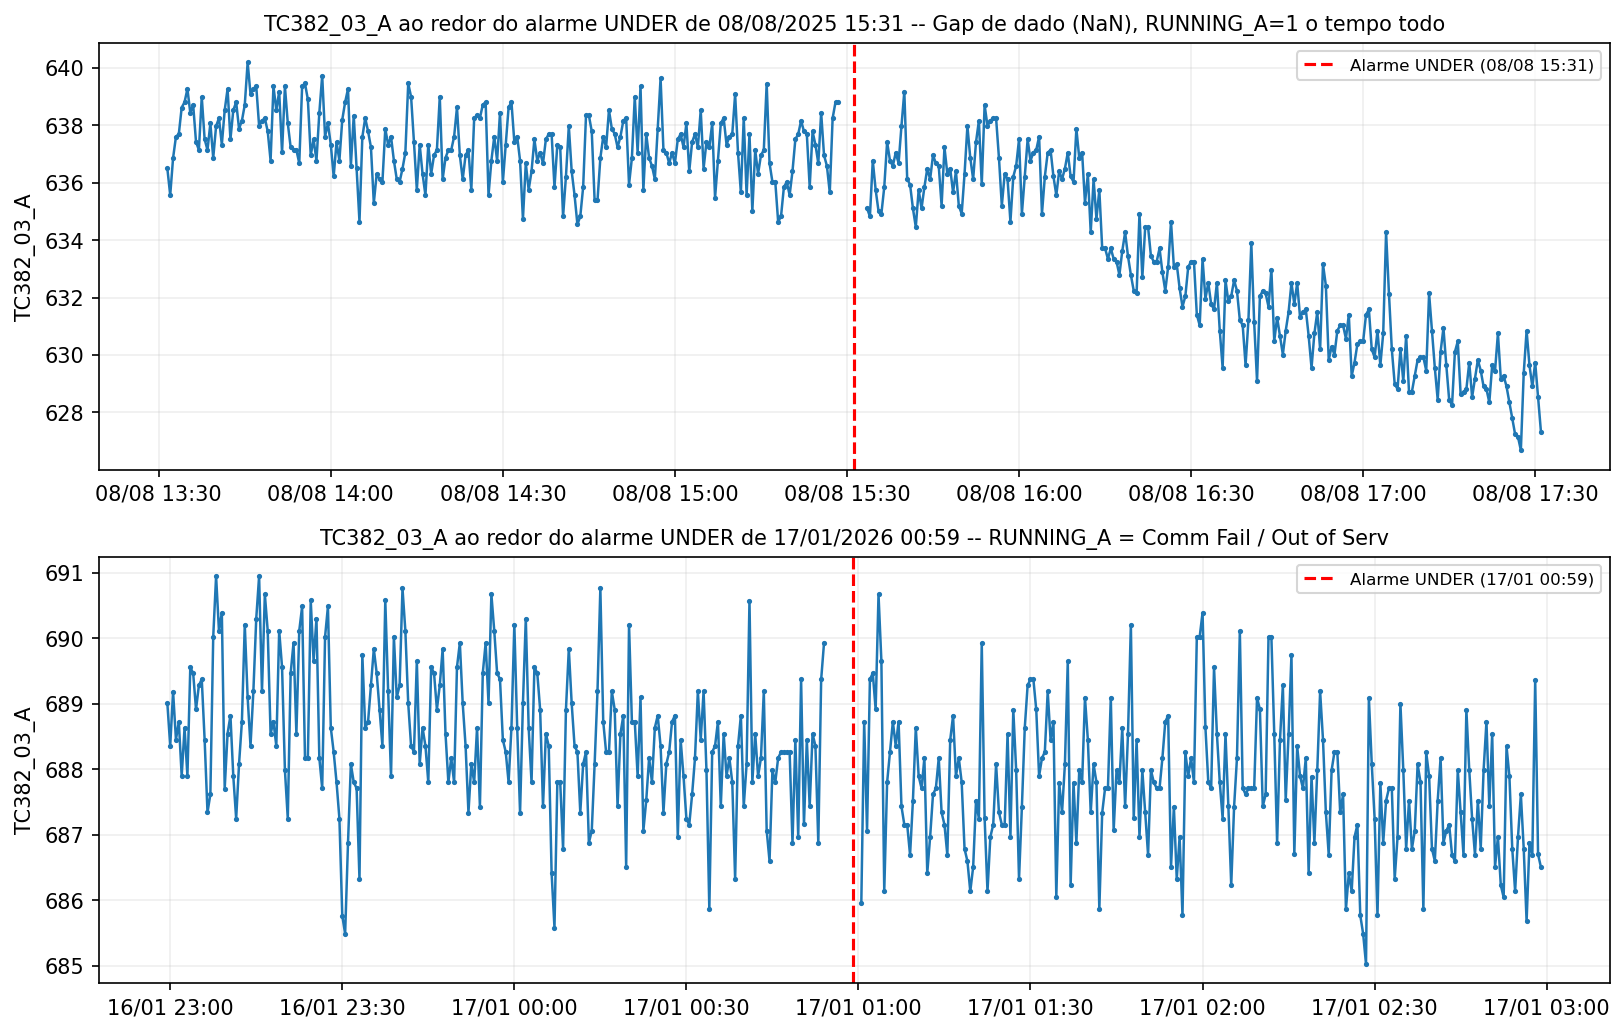
\includegraphics[width=\textwidth]{figs/exp7q/03_exemplos_under_sensor_error.png}
\caption{Dois dos cinco casos: \texttt{TC382\_03\_A} numa faixa
perfeitamente normal exatamente no instante em que o sistema de alarme
registrou $-21$/$-20$ -- a leitura que disparou o alarme nunca chegou ao
pipeline como valor de processo real.}
\end{figure}

\textbf{Não existe precursor de sensor para prever a própria falha de
comunicação do sensor.} Excluir UNDER não é viés de seleção -- é remover
alvos estruturalmente impossíveis de prever com os dados de
temperatura/vibração disponíveis.

\subsection{Métricas corrigidas: o que de fato conta como alarme real}

\begin{table}[H]
\centering
\begin{tabular}{@{}lcc@{}}
\toprule
\textbf{Métrica} & \textbf{Com UNDER (40)} & \textbf{Sem UNDER (32, real)} \\
\midrule
hit\_rate & 92,5\% & \textbf{100\%} \\
Antecedência real (preditivo) & 72,5\% (29/40) & \textbf{90,6\% (29/32)} \\
Reativo & 8 & 3 \\
Sem detecção & 3 & \textbf{0} \\
\bottomrule
\end{tabular}
\caption{Sobre os 32 alarmes genuínos, o candidato detecta 100\% deles com
90,6\% de antecedência real -- os 3 ``sem detecção'' eram exatamente os 3
UNDER mais problemáticos.}
\end{table}

\begin{figure}[H]
\centering
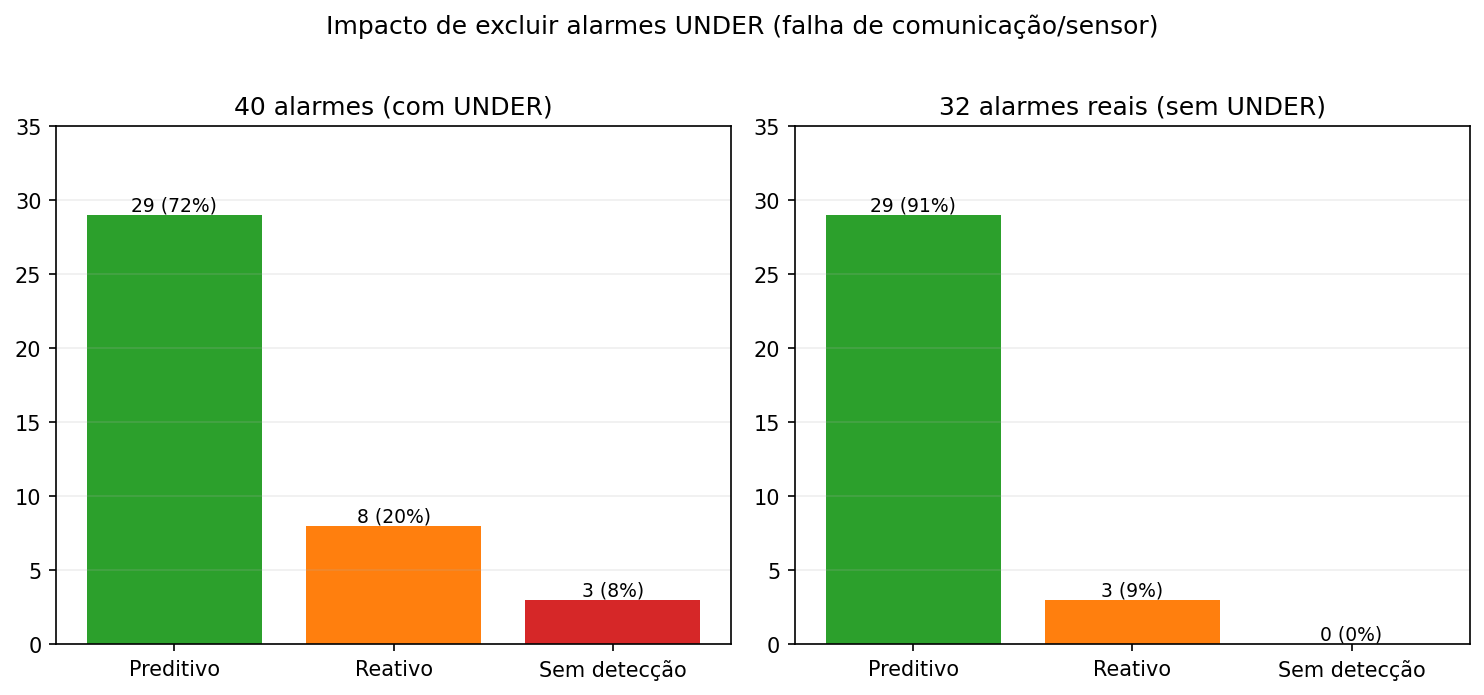
\includegraphics[width=\textwidth]{figs/exp7q/02_antes_depois_under.png}
\caption{Antes e depois de excluir UNDER -- zero casos sem detecção à
direita.}
\end{figure}

\subsection{Os 3 alarmes reativos remanescentes}
\label{sec:reativos}

Sobre os 32 alarmes genuínos, 3 continuam sendo detectados só depois do
alarme -- correspondem a apenas \textbf{2 eventos físicos distintos}.

\begin{table}[H]
\centering
\begin{tabular}{@{}llccc@{}}
\toprule
\textbf{Data/hora} & \textbf{Condição} & \textbf{Atraso até 1ª detecção} & \textbf{Evento} \\
\midrule
20/10/2025 16:18--16:20 & HI/HIHI & $\sim$4h & trip/religamento \\
24/02/2026 11:01 & HI & 0min (simultâneo) & início tipo degrau \\
\bottomrule
\end{tabular}
\end{table}

\textbf{Evento 1 (trip/religamento):} o estado operacional sai de
\texttt{"on"} \textbf{antes} do próprio alarme e oscila entre
\texttt{"transiente"}/\texttt{"off\_curto"} por quase 5h -- a pipeline zera
\texttt{is\_anom\_point} por design nesses estados. A 1ª detecção só
aparece quando o estado volta a \texttt{"on"} estável -- não é
coincidência, é a mecânica exata da máscara operacional.

\begin{figure}[H]
\centering
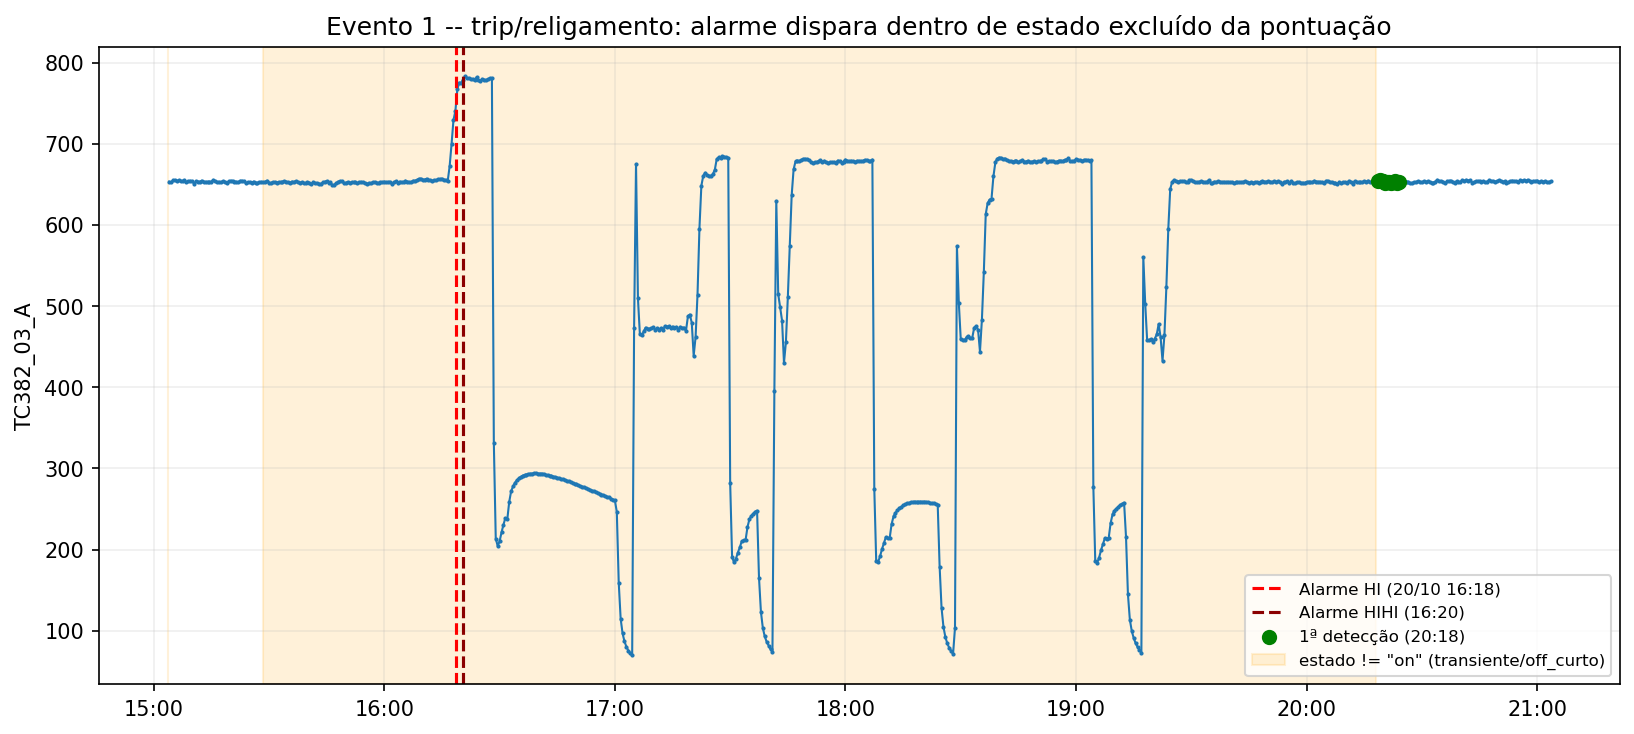
\includegraphics[width=\textwidth]{figs/exp7q/06_evento_trip_reativo.png}
\caption{\texttt{TC382\_03\_A} ao redor do trip de 20/10/2025. Áreas
sombreadas = estado $\neq$ \texttt{"on"}; a detecção (ponto verde) só
ocorre quando o estado volta a \texttt{"on"}.}
\end{figure}

\textbf{Evento 2 (início tipo degrau):} \texttt{operational\_state="on"} o
tempo todo. \texttt{TC382\_03\_A} fica estável por $\geq$6h antes do
alarme, sem sinal gradual, e salta abruptamente -- sem precursor visível
em nenhuma das 4 escalas de tempo capturadas.

\begin{figure}[H]
\centering
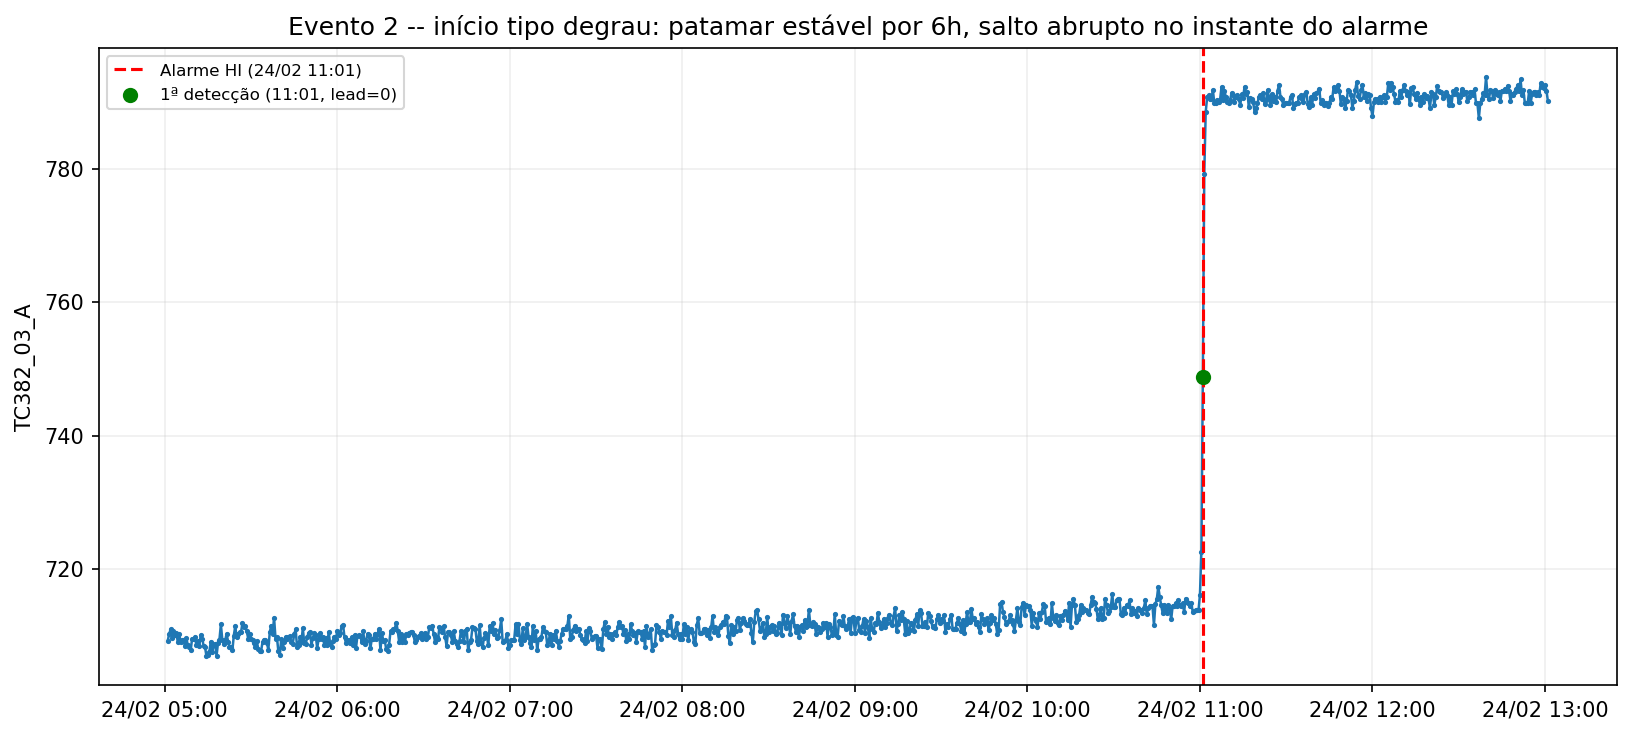
\includegraphics[width=\textwidth]{figs/exp7q/07_evento_degrau_reativo.png}
\caption{Patamar estável por 6h, depois salto abrupto coincidente com o
próprio alarme -- a 1ª detecção ocorre no mesmo intervalo do alarme, o
mais rápido possível dado o grid de debounce.}
\end{figure}

\textbf{Síntese: nenhum dos 3 casos reativos indica falha de engenharia de
features a corrigir} -- um é limite estrutural de escopo (transiente de
partida/parada excluído por design), o outro é evento genuinamente sem
antecedência física possível.

% =====================================================================
\clearpage
\part{EXP10: do candidato final de temperatura ao falso alerta residual}
\label{part:exp10}
% =====================================================================

% ---------------------------------------------------------------------
\section{Ponto de partida}
% ---------------------------------------------------------------------

Candidato de referência ao final do EXP7: \texttt{ocsvm} (p99,9/debounce=1),
multiescala + textura -- \textbf{92,5\% hit\_rate, 1,94\% de falso
alerta} (base de 40 alarmes, consistente com a Parte~\ref{part:exp7}). O
EXP10 \textbf{não mexe no modelo}: investiga a \emph{estrutura} do falso
alerta residual em vez de tratá-lo como ruído agregado, e ataca 3 causas
distintas, uma de cada vez -- sem perder nenhum dos 37 alarmes já
detectados em nenhuma etapa.

\textbf{Método:} fragmentação da série \texttt{is\_anom\_point} em
episódios contínuos (gap $\leq$5 min), cruzados com dados brutos e com o
catálogo completo de 47 tags de alarme. Achado estrutural: 72,5\% dos
12.782 pontos de falso alerta (OOS) se concentram em apenas 10 dos 295
episódios.

% ---------------------------------------------------------------------
\section{Achado 1 (EXP10): desligamento real que a máscara não via}
% ---------------------------------------------------------------------

Os 5 maiores episódios (19--24/08/2025) coincidem com
\texttt{TC382\_03\_A} caindo de $\sim$478°C para $\sim$28--32°C por 3,5
dias, enquanto \texttt{RUNNING\_A} permanece $\sim$0,96--1,0 o tempo todo
-- a máscara nunca excluía esse período. Confirmado como desligamento real
via alarmes de pressão/partida a gás do catálogo completo, disparando
exatamente nas bordas do período.

\begin{figure}[H]
\centering
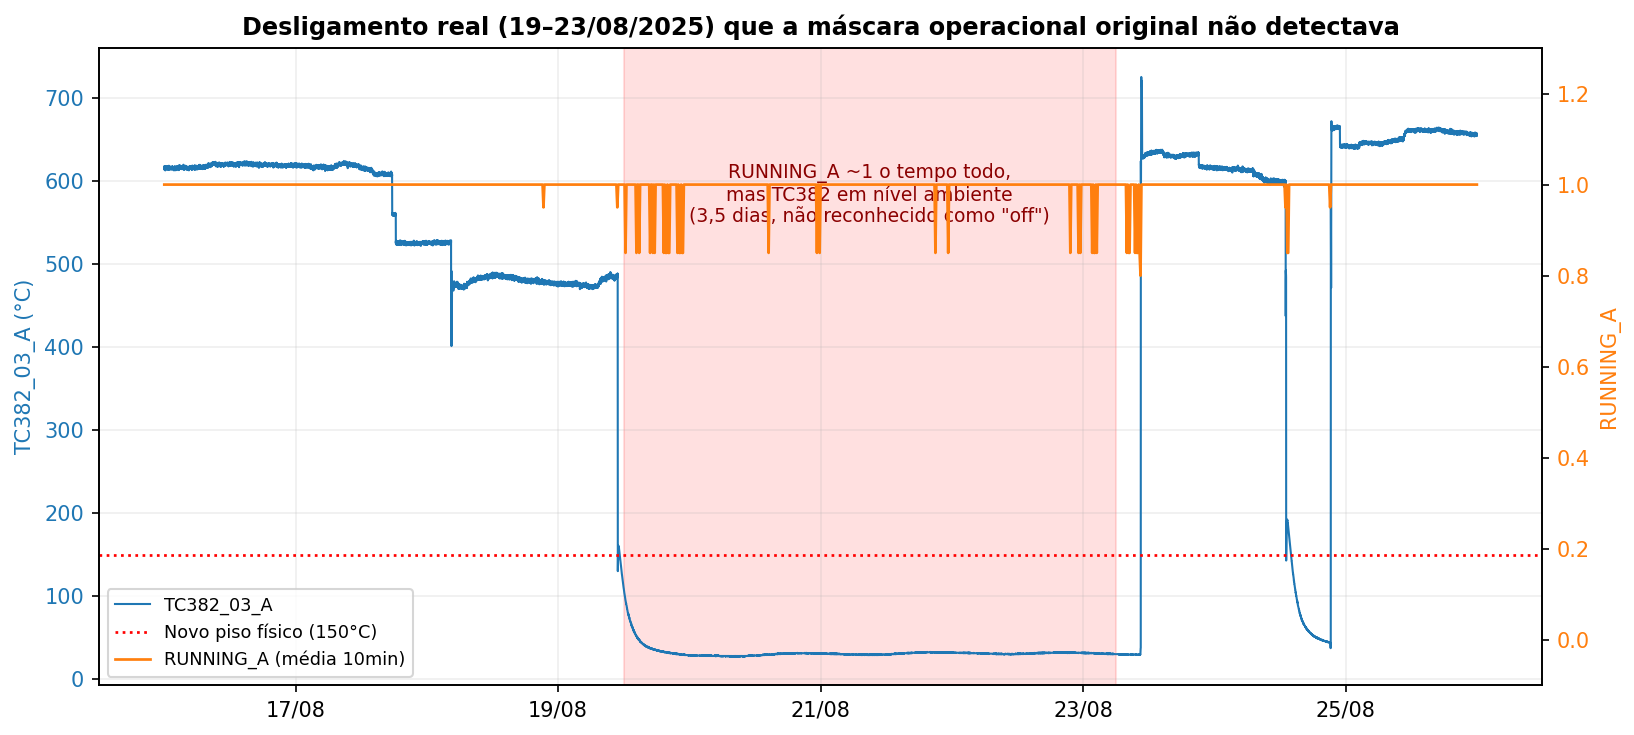
\includegraphics[width=\textwidth]{figs/exp10/03_desligamento_mal_rotulado.png}
\caption{O episódio de 19--24/08/2025: temperatura caindo para a faixa de
desligamento enquanto \texttt{RUNNING\_A} permanece perto de 1.}
\end{figure}

\textbf{Correção:} \texttt{build\_operational\_state}
(\texttt{src/cnn1d\_ae/scoring.py}) ganhou \texttt{secondary\_series}/
\texttt{secondary\_off\_abs\_threshold} -- o próprio sensor-alvo do grupo
caindo abaixo de um piso físico (\texttt{OFF\_TARGET\_ABS\_THRESHOLD},
150°C) também conta como ``off'', unido por OR ao critério de
\texttt{OPERATIONAL\_REF\_SENSOR}, antes da classificação
off\_curto/off\_longo/transiente já existente.

\begin{figure}[H]
\centering
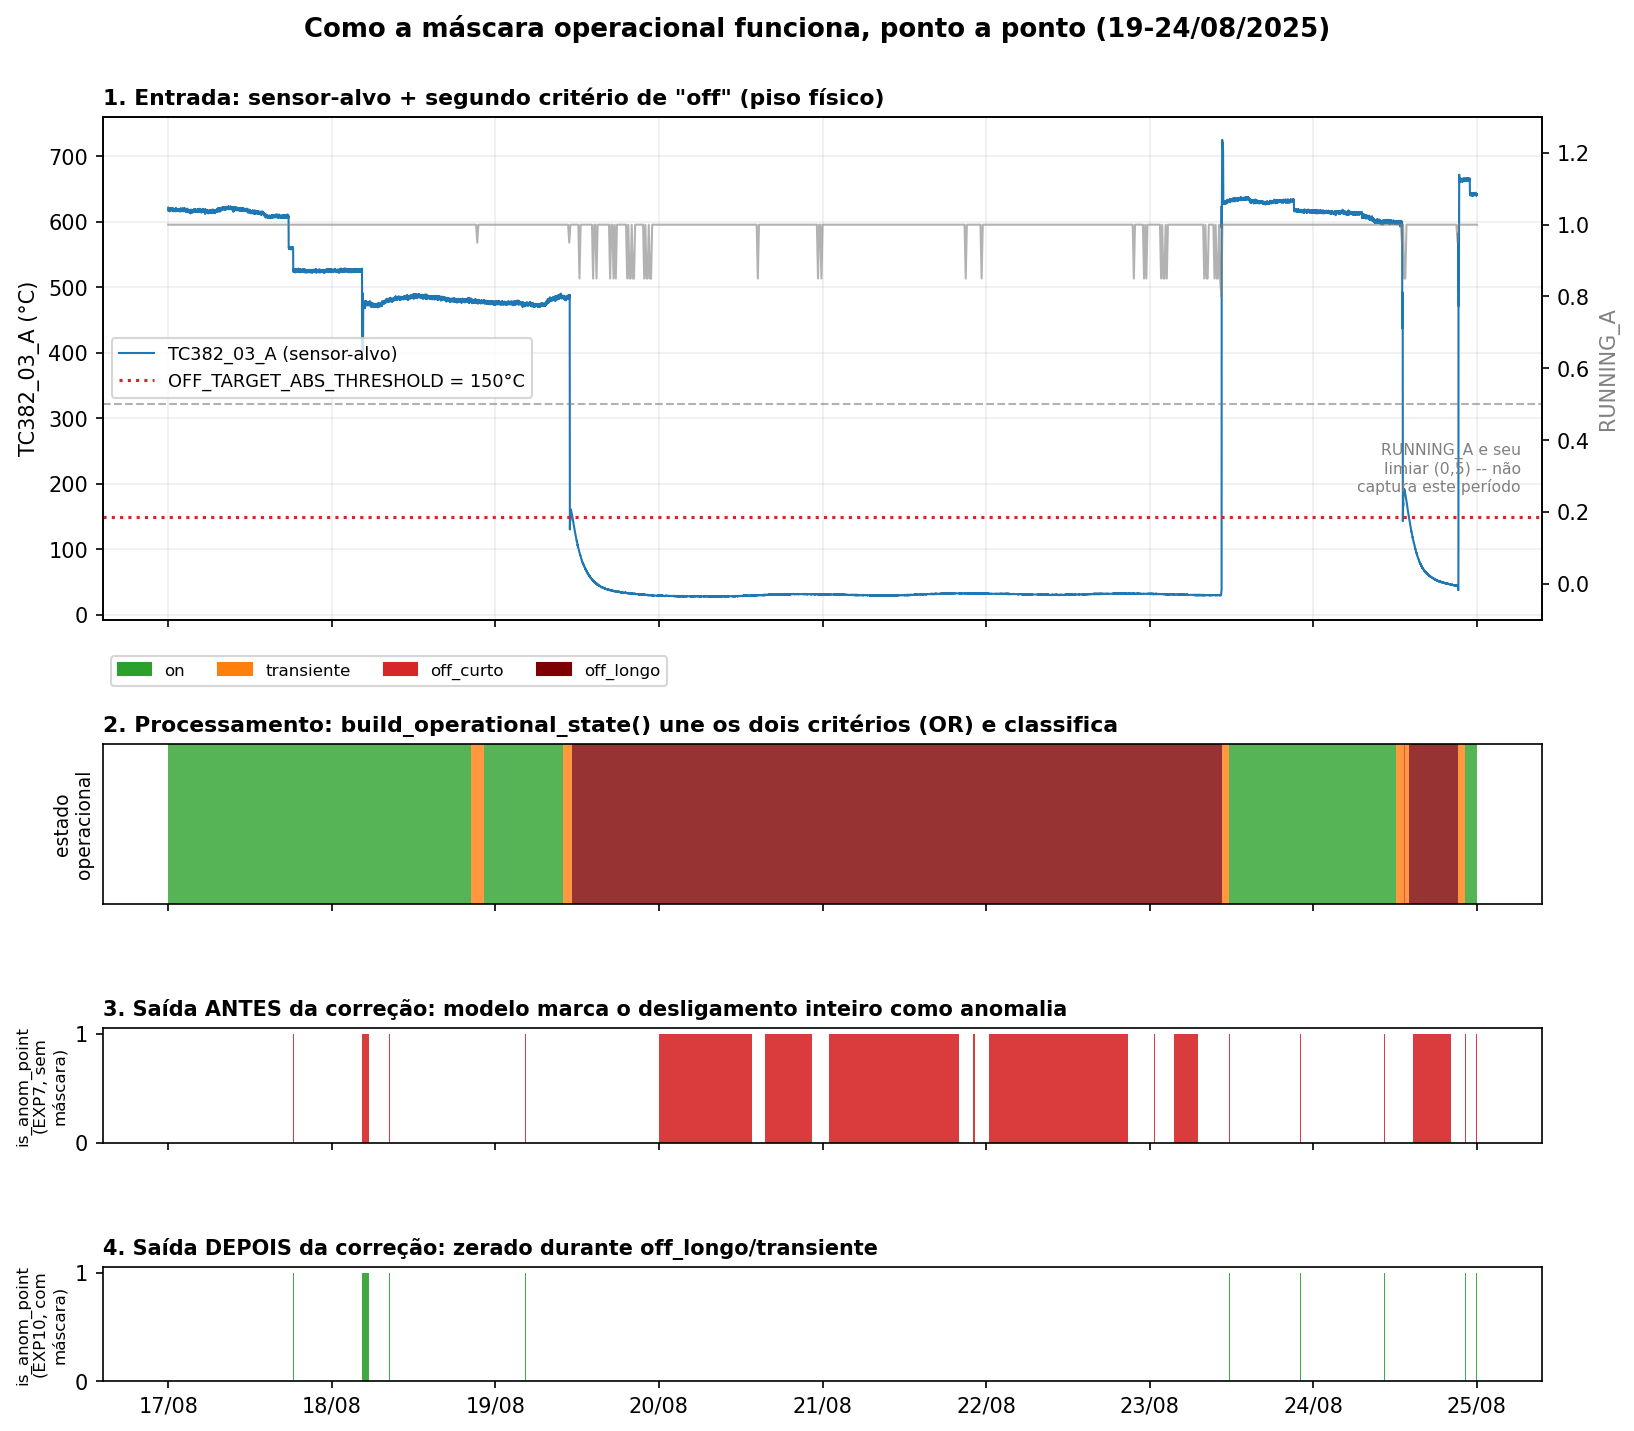
\includegraphics[width=0.92\textwidth]{figs/exp10/12_mecanismo_mascara_operacional.png}
\caption{Esquema do mecanismo: quando o sensor-alvo cai abaixo do piso
físico (linha tracejada), o novo critério classifica o período como
``off'' mesmo que o sensor de referência primário não tenha capturado a
mudança -- suprimindo o falso alerta desse trecho.}
\end{figure}

\textbf{Resultado (EXP10): hit\_rate idêntico (92,5\%, 37/40); FP
1,94\%$\to$0,67\%.} Seed-sweep: desvio-padrão de 0,019pp.

\subsection*{Caminho testado e descartado: debounce}

Simulação offline da grade de debounce (1 a 60) mostrou ganho de FP
pequeno até debounce=10 (1,94\%$\to$1,66\%, já custando 3 preditivos) e
perda de alarmes reais inteiros além disso. Causa: a duração mediana dos
episódios de FP residual (6 pontos/2,5min) se sobrepõe à dos episódios
mais curtos que ainda precedem um alarme real (25º percentil = 6min).
Debounce não separa os dois.

\begin{figure}[H]
\centering
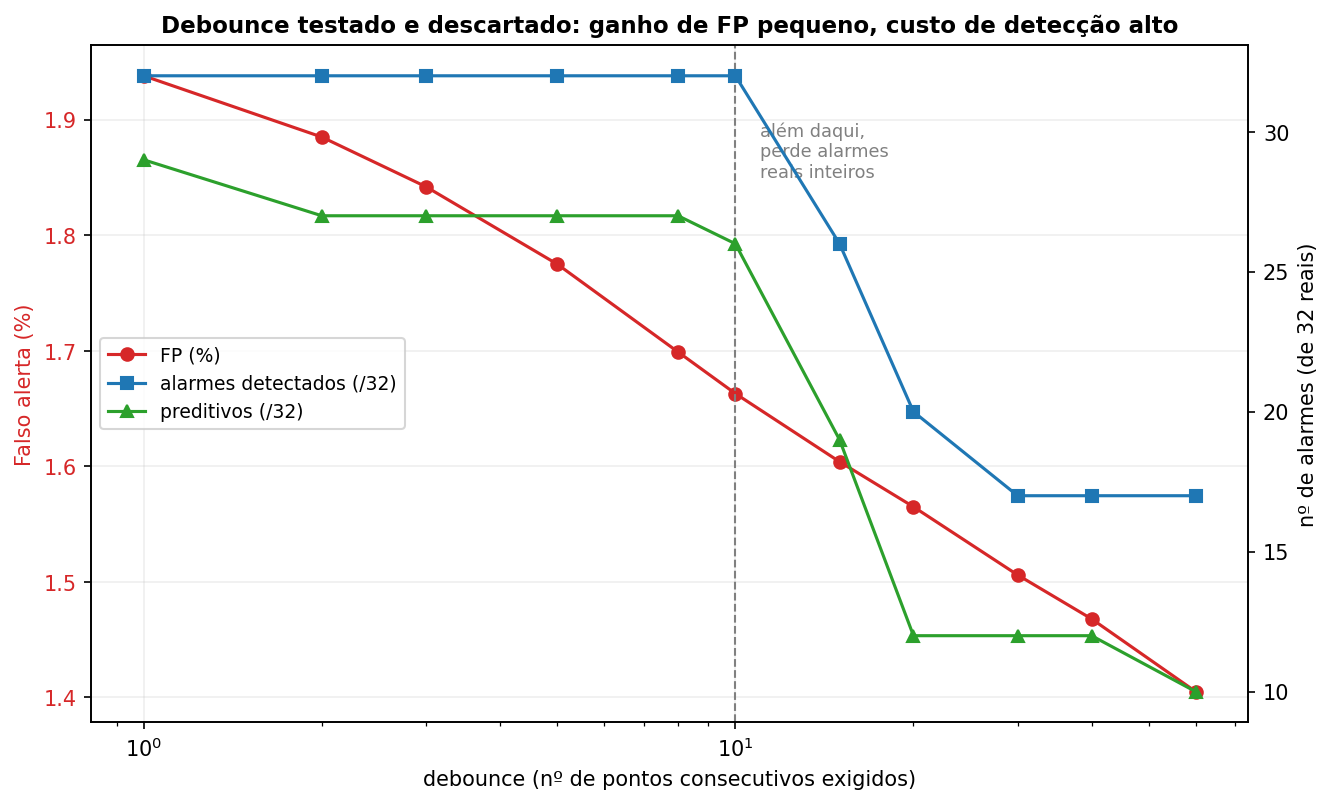
\includegraphics[width=0.85\textwidth]{figs/exp10/06_grade_debounce_descartada.png}
\caption{Grade de debounce: o ganho de FP não compensa a perda de
preditivos além de debounce$\approx$10.}
\end{figure}

% ---------------------------------------------------------------------
\section{Achado 2 (EXP10b): rampas de carga reais}
% ---------------------------------------------------------------------

Dos 4.441 pontos de FP residual (287 episódios), a variabilidade local de
\texttt{TC382\_03\_A} é 5--9$\times$ maior que em pontos normais (nível
idêntico -- não é viés de faixa). Investigação individual dos 10 maiores
episódios: 8 de 10 mostram \texttt{TC382\_03\_A}/\texttt{T5\_AVG\_A}
variando dezenas de graus em $\sim$1h, com desvio-padrão de vibração
3--6$\times$ mais alto -- manobra de carga real, sem alarme, sem falha.

\begin{figure}[H]
\centering
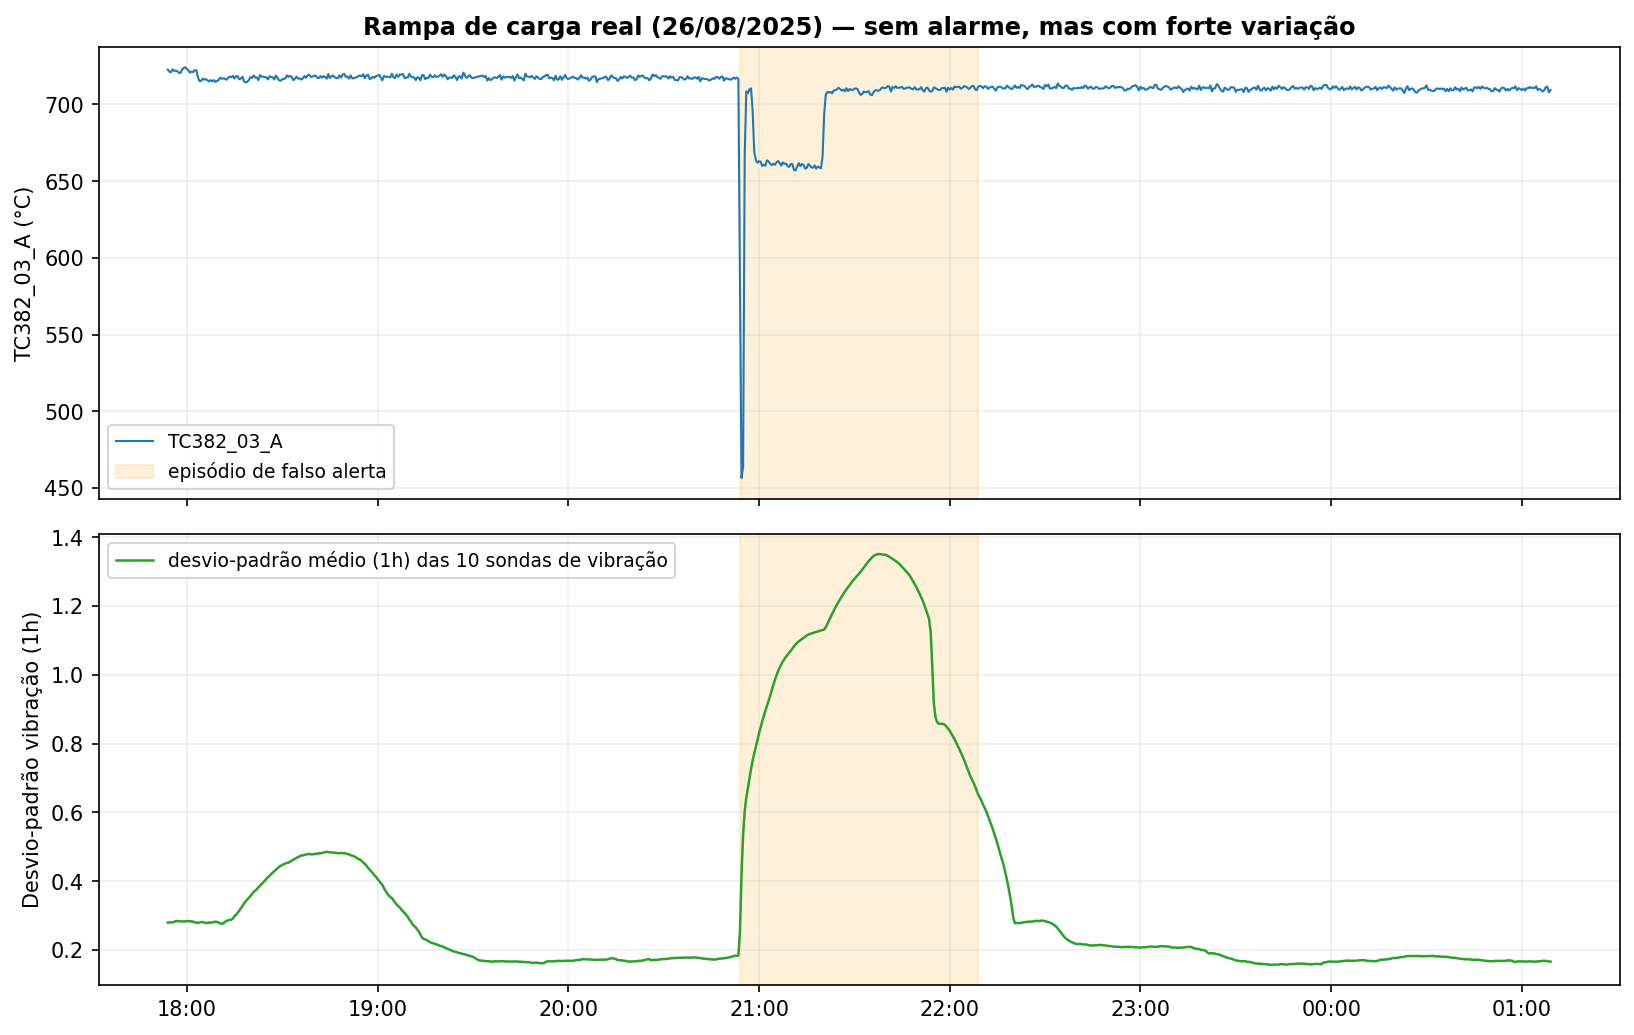
\includegraphics[width=\textwidth]{figs/exp10/04_rampa_carga_exemplo.png}
\caption{Exemplo de rampa de carga legítima: variação de dezenas de graus
em $\sim$1h, sem alarme correspondente.}
\end{figure}

\textbf{Correção:} \texttt{ENABLE\_LOAD\_GATE}/\texttt{apply\_load\_gate}
já existia para o CNN1D-AE (pipeline sequencial, produção) mas nunca fora
portado ao AutoML -- portado aqui. Parâmetros default do CNN1D-AE
(halflife=120min/janela=360min) custavam até 6 casos preditivos -- uma
rampa de falha real e uma rampa de carga legítima têm a mesma assinatura
de taxa de variação numa janela longa. Janela curta (halflife=15min/
janela=30min) + \texttt{ramp\_max=100°C/h} preservam 29/29 preditivos.

\begin{figure}[H]
\centering
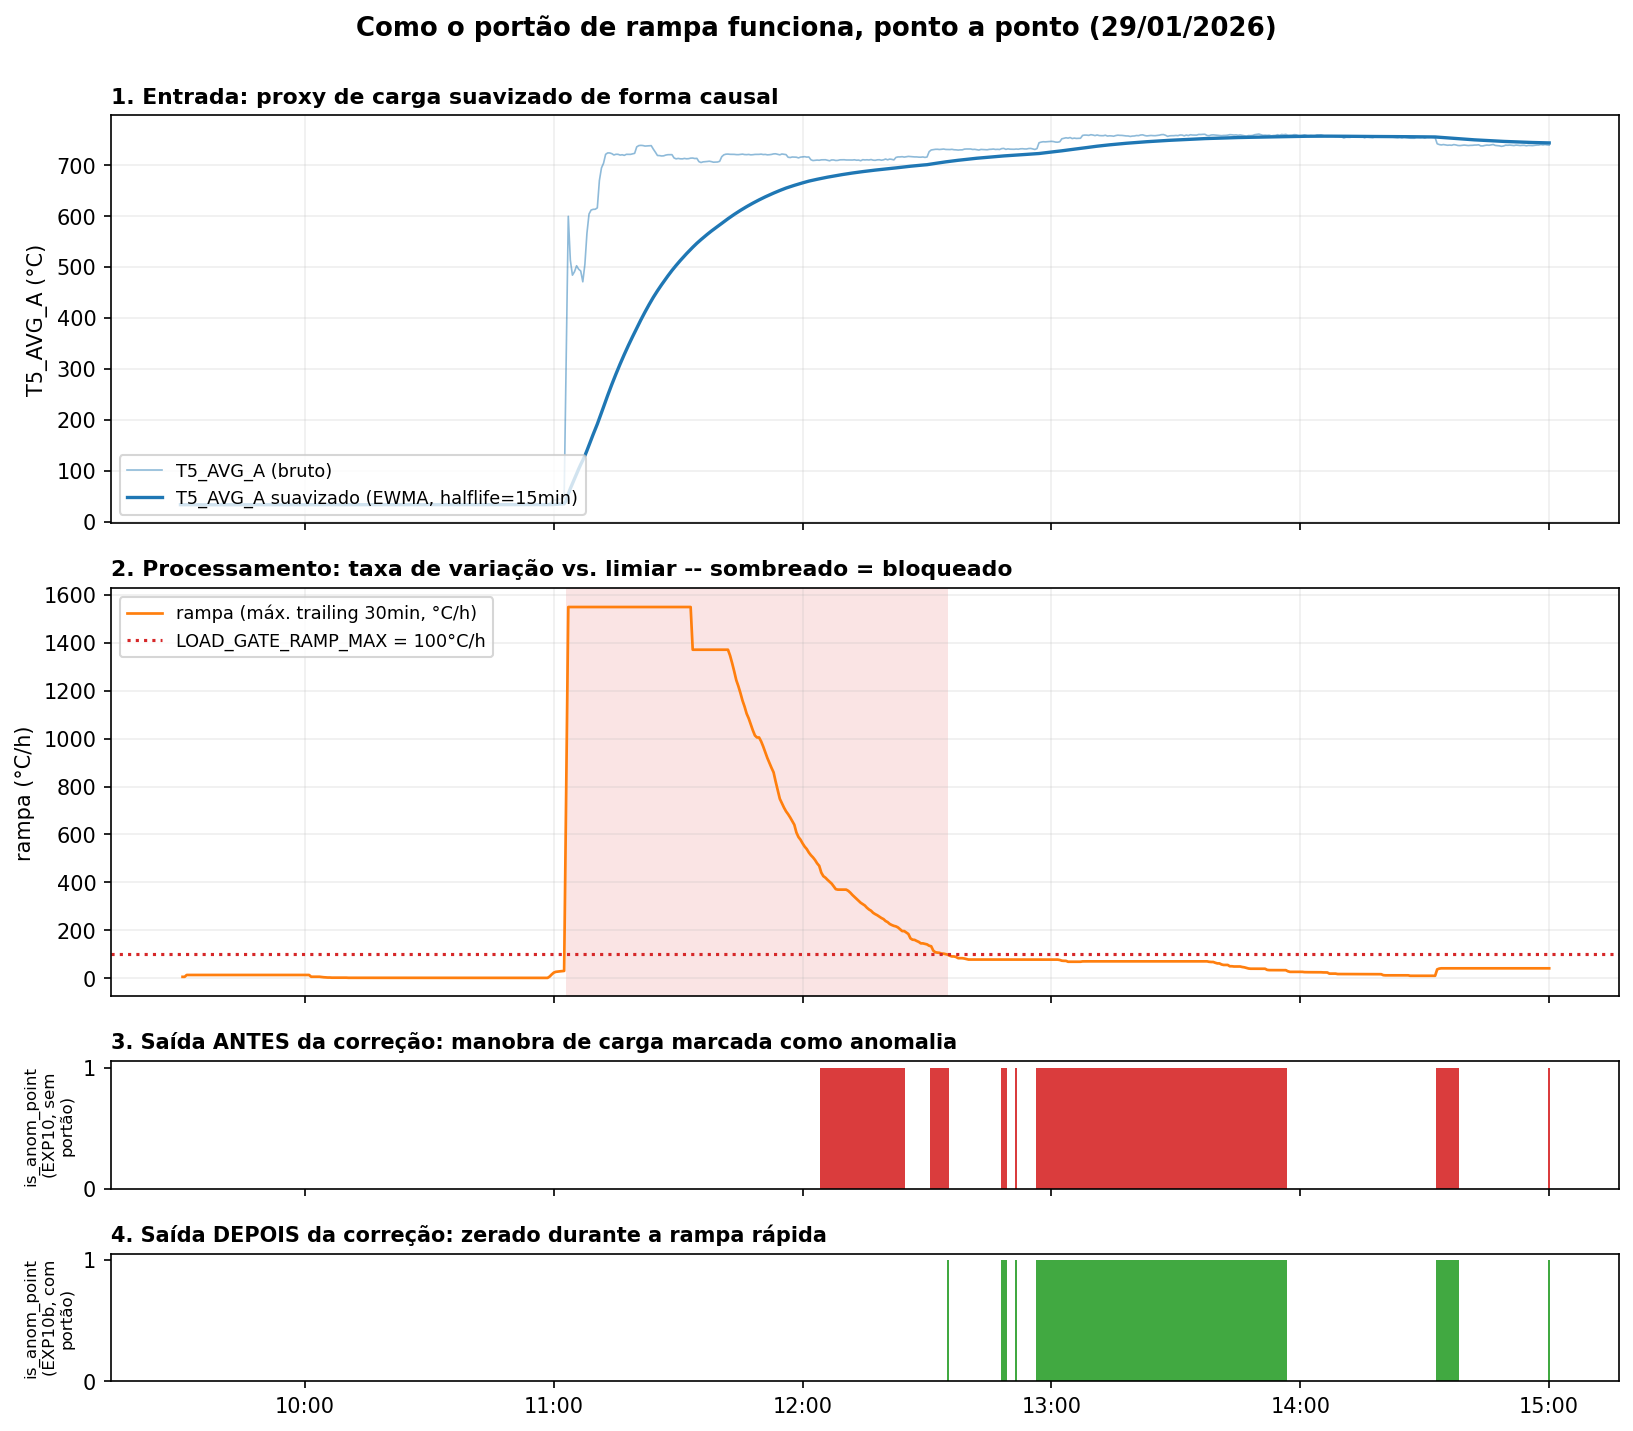
\includegraphics[width=0.92\textwidth]{figs/exp10/13_mecanismo_portao_rampa.png}
\caption{Esquema: quando a taxa de variação suavizada do proxy de carga
ultrapassa o limiar, \texttt{is\_anom\_point} é suprimido durante a
manobra -- janela curta o bastante para não confundir com uma rampa de
falha real.}
\end{figure}

\begin{figure}[H]
\centering
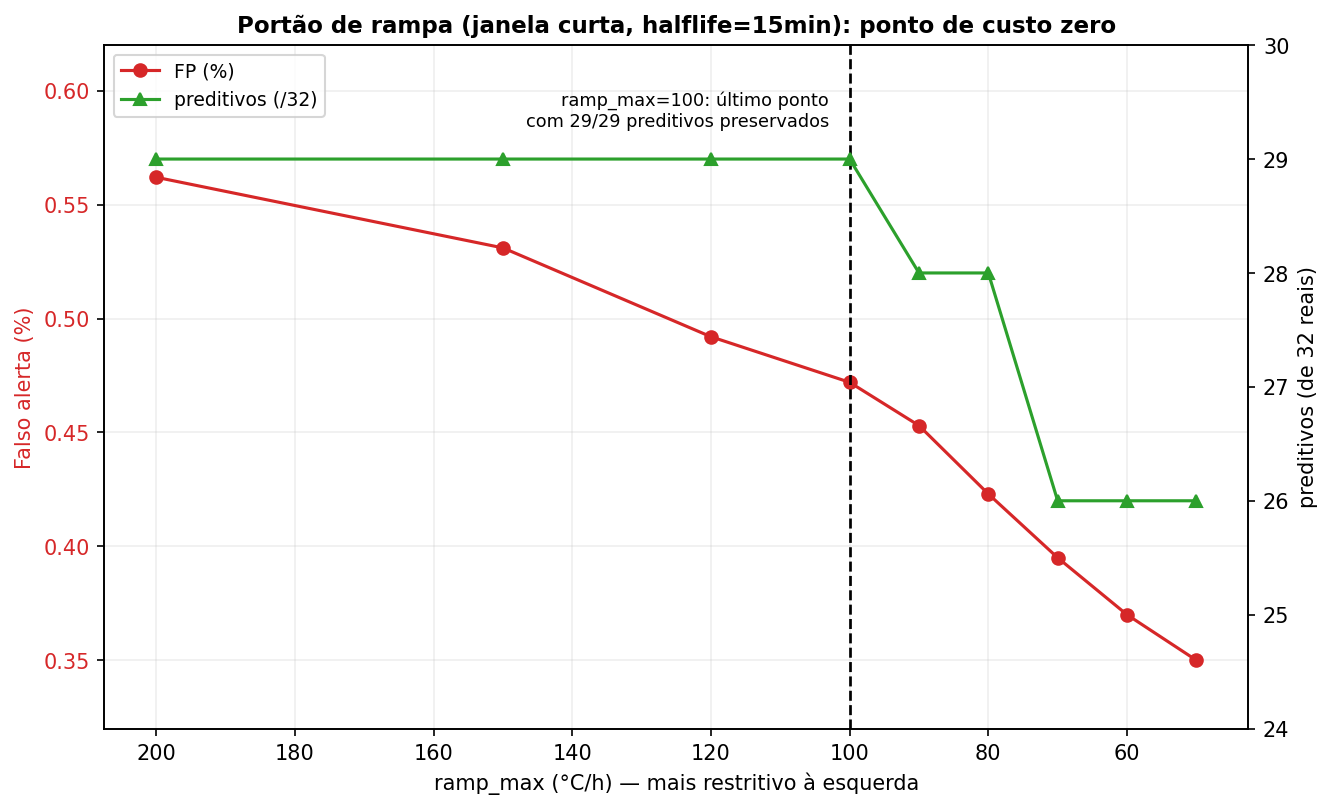
\includegraphics[width=0.85\textwidth]{figs/exp10/07_portao_rampa_ramp_max.png}
\caption{Sensibilidade ao parâmetro \texttt{ramp\_max}: ponto escolhido
preserva todos os preditivos.}
\end{figure}

\textbf{Resultado (EXP10b): hit\_rate idêntico (92,5\%, 37/40); FP
0,67\%$\to$0,48\%.} Seed-sweep: desvio-padrão de 0,016pp.

% ---------------------------------------------------------------------
\section{Achado 3 (EXP10c): volatilidade que persiste, não que sobe}
% ---------------------------------------------------------------------

O portão de rampa reage bem a variação de \emph{nível}, mas o padrão de
vibração do Achado 2 é diferente: o desvio-padrão sobe e \textbf{permanece}
elevado por 1--2h, não é só um pico na subida.

\textbf{Tentativa 1 (falhou):} alimentar \texttt{apply\_load\_gate} com um
índice de volatilidade de vibração no lugar do proxy de temperatura,
mantendo o mecanismo de taxa de variação -- reduzia o FP de 0,480\% para
apenas 0,477\%: taxa de variação não distingue início de rampa real de
início de escalada de falha, mesmo problema do portão original, causa
relacionada mas distinta (métrica errada, não janela errada).

\textbf{Tentativa 2 (funcionou):} \texttt{compute\_volatility\_index}/
\texttt{apply\_volatility\_gate} -- desvio-padrão móvel causal
(\texttt{VOLATILITY\_GATE\_WINDOW\_MINUTES=60min}) de cada um dos 10
canais de vibração, reduzido pela média entre canais, bloqueando quando o
\textbf{nível} (não a taxa) ultrapassa \texttt{VOLATILITY\_GATE\_THRESHOLD}.
Simulação offline encontrou \texttt{threshold=0,39} como ponto de custo
zero: preserva 29/29 preditivos com FP caindo 27\% relativo.

\begin{figure}[H]
\centering
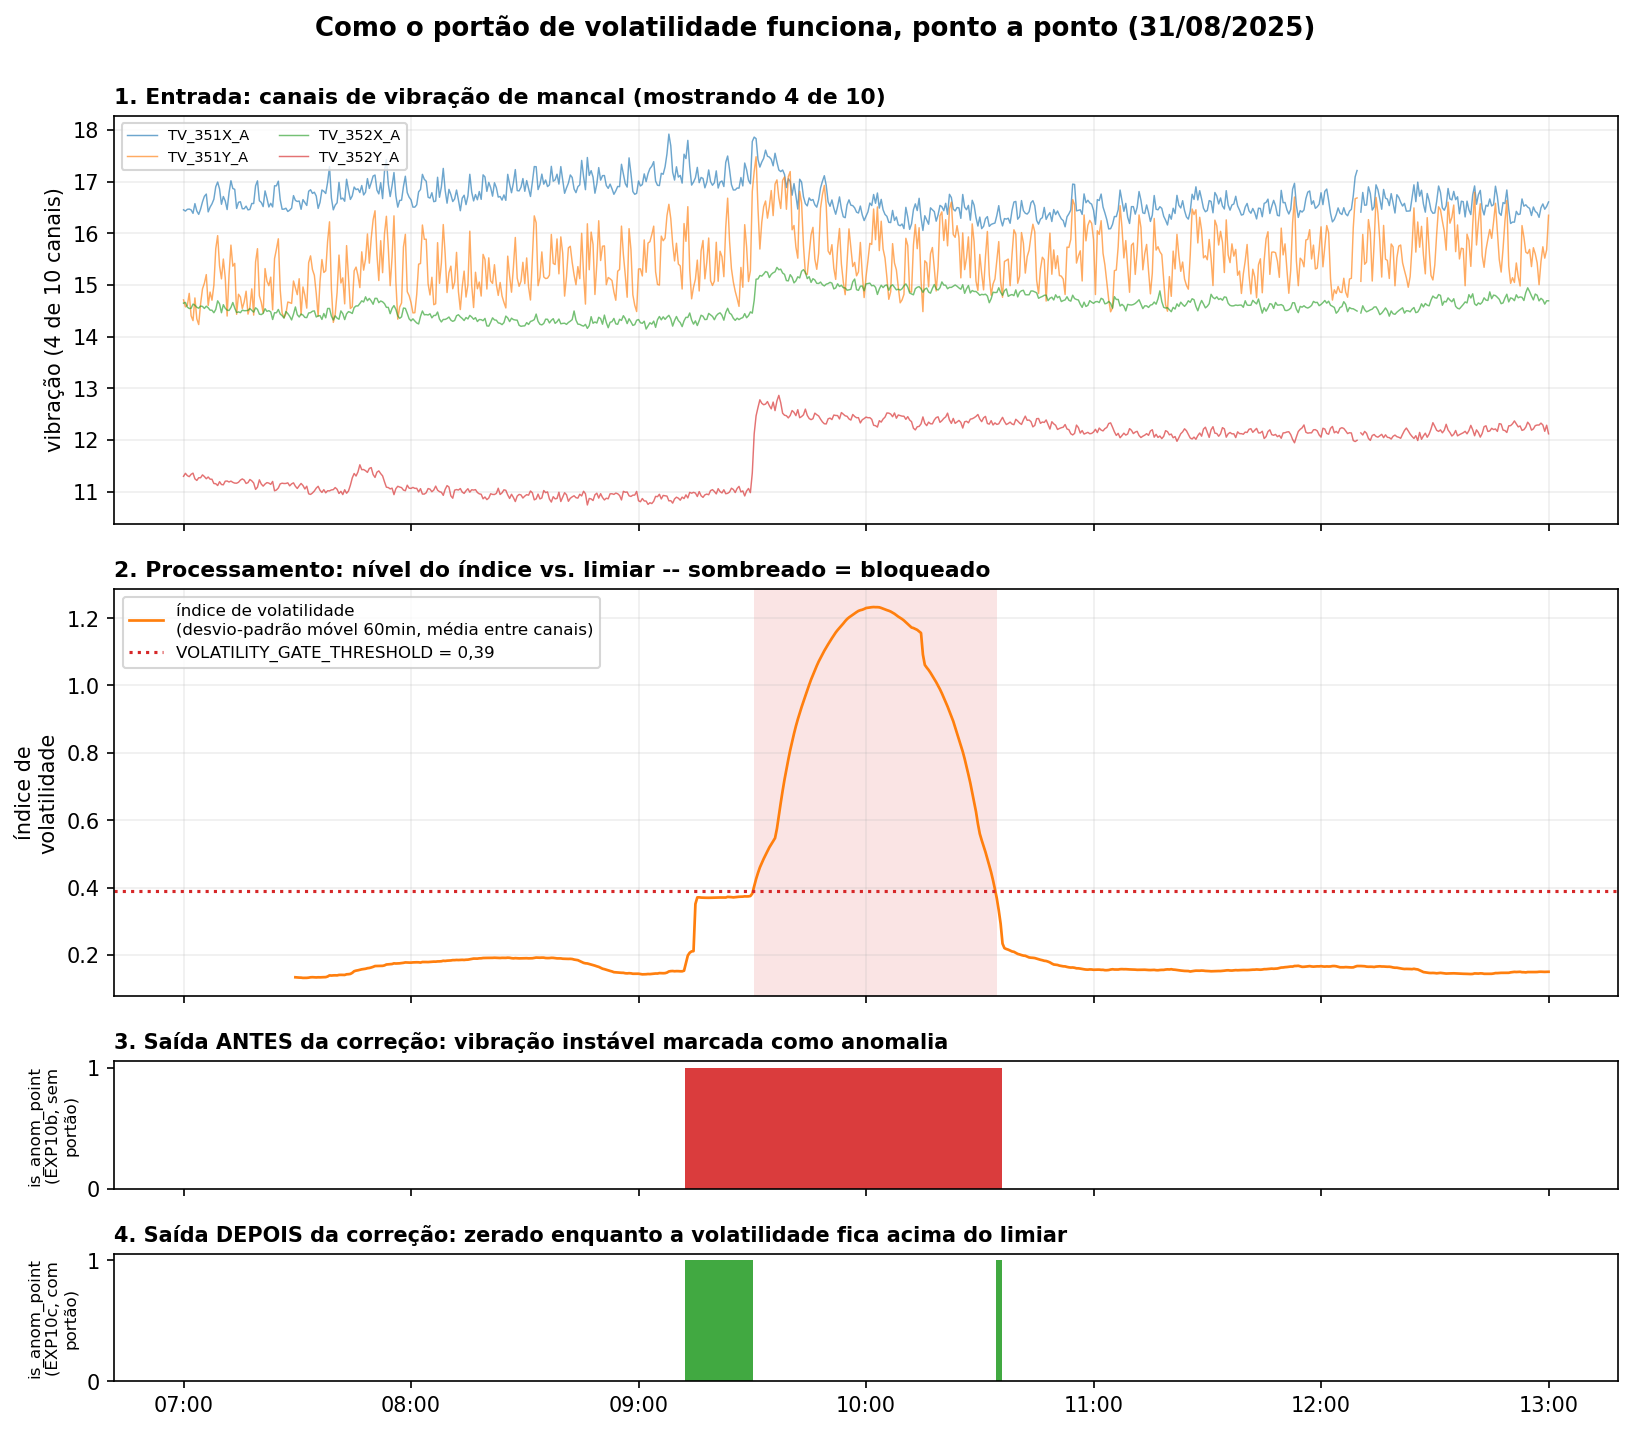
\includegraphics[width=0.92\textwidth]{figs/exp10/14_mecanismo_portao_volatilidade.png}
\caption{Esquema: o índice de volatilidade (média entre os 10 canais de
vibração) permanece elevado por toda a manobra, não só no início -- o
portão bloqueia enquanto o nível estiver acima do limiar, não só na
subida.}
\end{figure}

\begin{figure}[H]
\centering
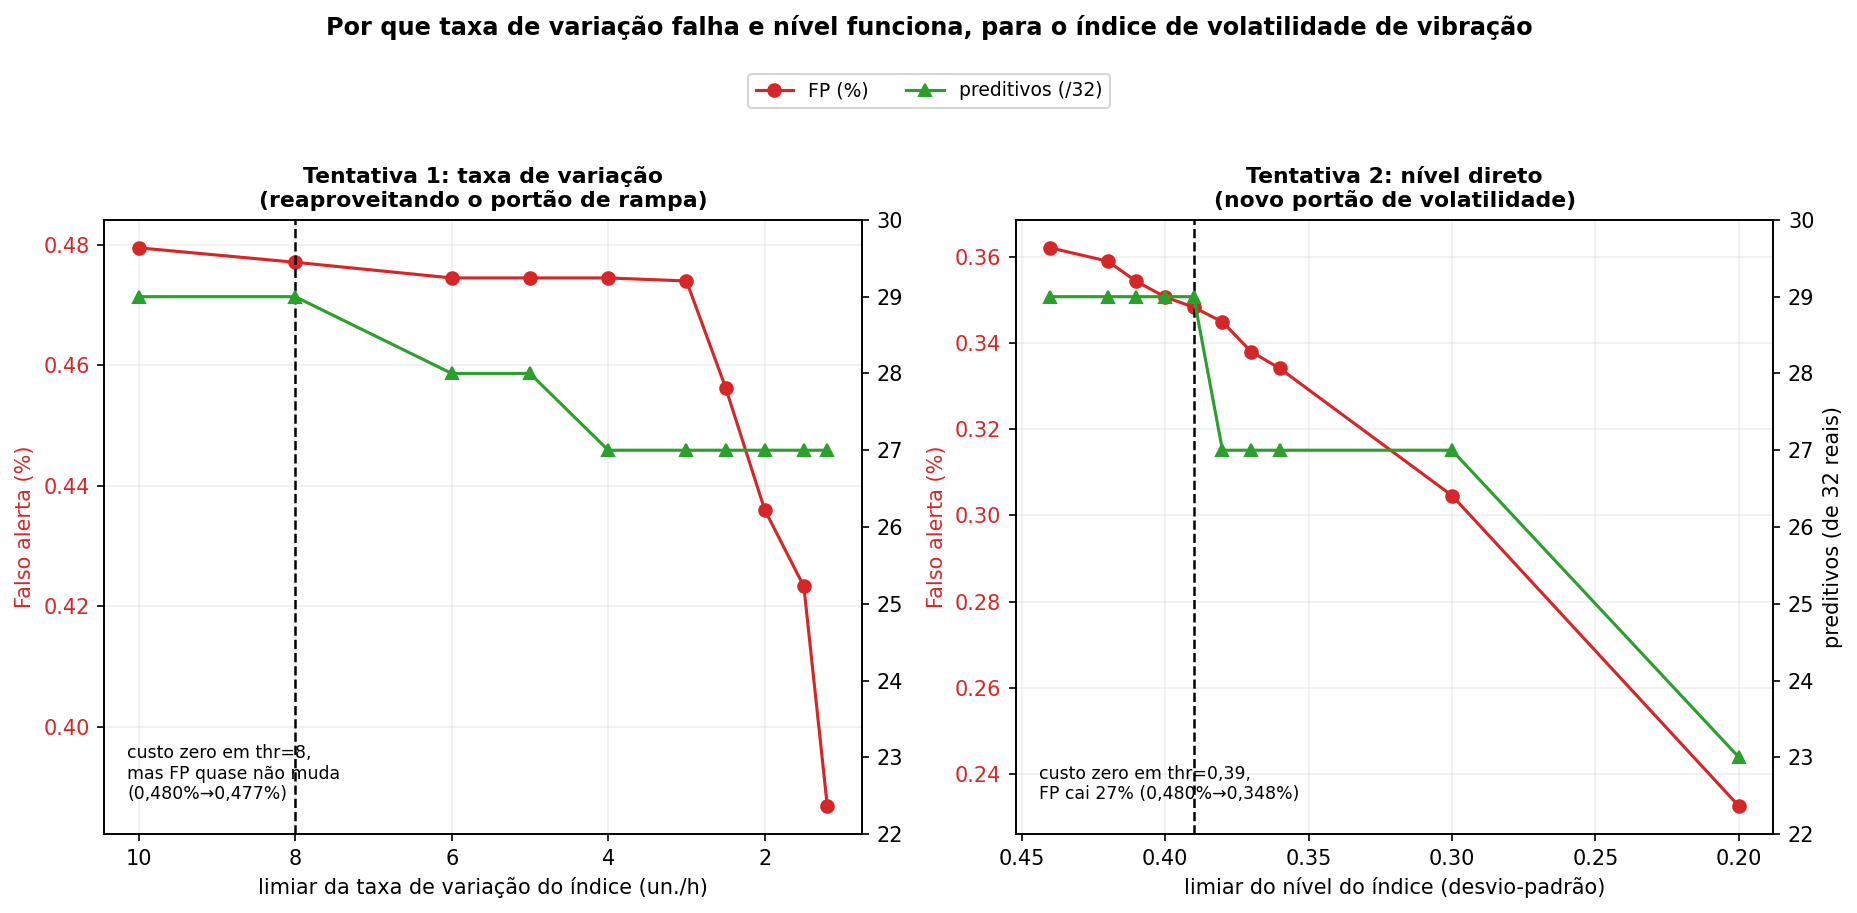
\includegraphics[width=\textwidth]{figs/exp10/10_portao_volatilidade_comparacao.png}
\caption{Comparação do índice de volatilidade antes/depois do portão --
episódios de falso alerta residual coincidem com volatilidade sustentada
acima do limiar.}
\end{figure}

\textbf{Resultado (EXP10c): hit\_rate idêntico (92,5\%, 37/40); FP
0,48\%$\to$0,35\%.} Seed-sweep: desvio-padrão de 0,011pp.

% ---------------------------------------------------------------------
\section{Resultado consolidado: o sensor-alvo, antes e depois}
% ---------------------------------------------------------------------

\begin{table}[H]
\centering
\begin{tabular}{@{}lcc@{}}
\toprule
\textbf{Etapa} & \textbf{hit\_rate} & \textbf{FP} \\
\midrule
EXP7 item1+2 (base) & 92,5\% (37/40) & 1,94\% \\
EXP10 (+ máscara operacional) & 92,5\% (37/40) & 0,67\% \\
EXP10b (+ portão de rampa) & 92,5\% (37/40) & 0,48\% \\
\textbf{EXP10c (+ portão de volatilidade)} & \textbf{92,5\% (37/40)} & \textbf{0,35\%} \\
\bottomrule
\end{tabular}
\caption{Redução total de falso alerta: 1,94\%$\to$0,35\% (\textbf{82\%
relativo}), com \textbf{zero} custo de detecção em qualquer etapa.}
\end{table}

A Figura~\ref{fig:serie-antes-depois} mostra o \textbf{sensor-alvo}
diretamente: um trecho da série completa onde havia falso alerta antes das
3 correções, e a mesma janela depois -- os pontos de FP desaparecem sem
que nenhum ponto de detecção real seja afetado.

\begin{figure}[H]
\centering
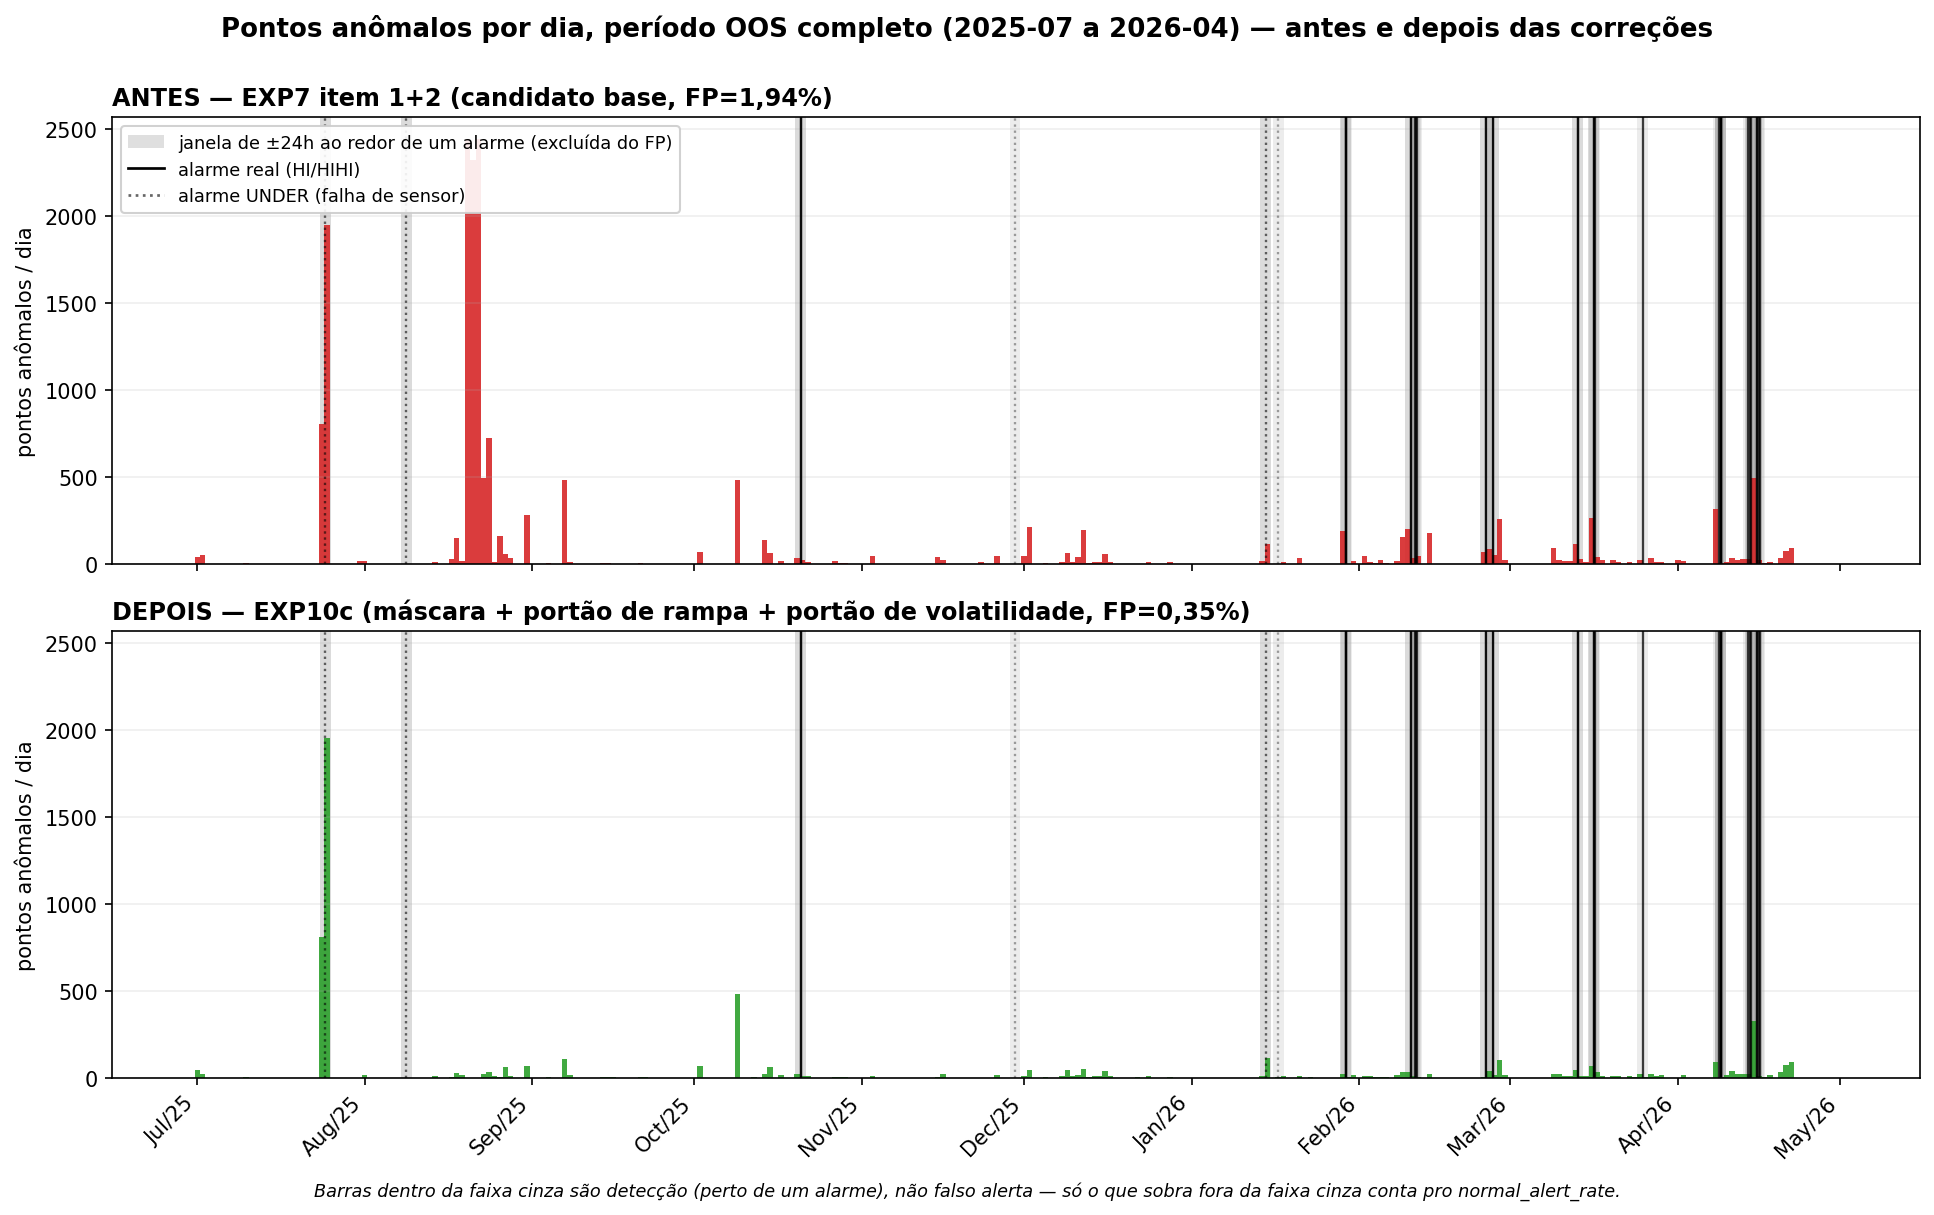
\includegraphics[width=\textwidth]{figs/exp10/08_serie_completa_antes_depois.png}
\caption{Série completa de \texttt{TC382\_03\_A}, antes (topo) e depois
(embaixo) dos 3 filtros -- os episódios de falso alerta concentrados em
2025-08 e outras janelas somem; os alarmes reais (linhas verdes) continuam
todos detectados.}
\label{fig:serie-antes-depois}
\end{figure}

\begin{figure}[H]
\centering
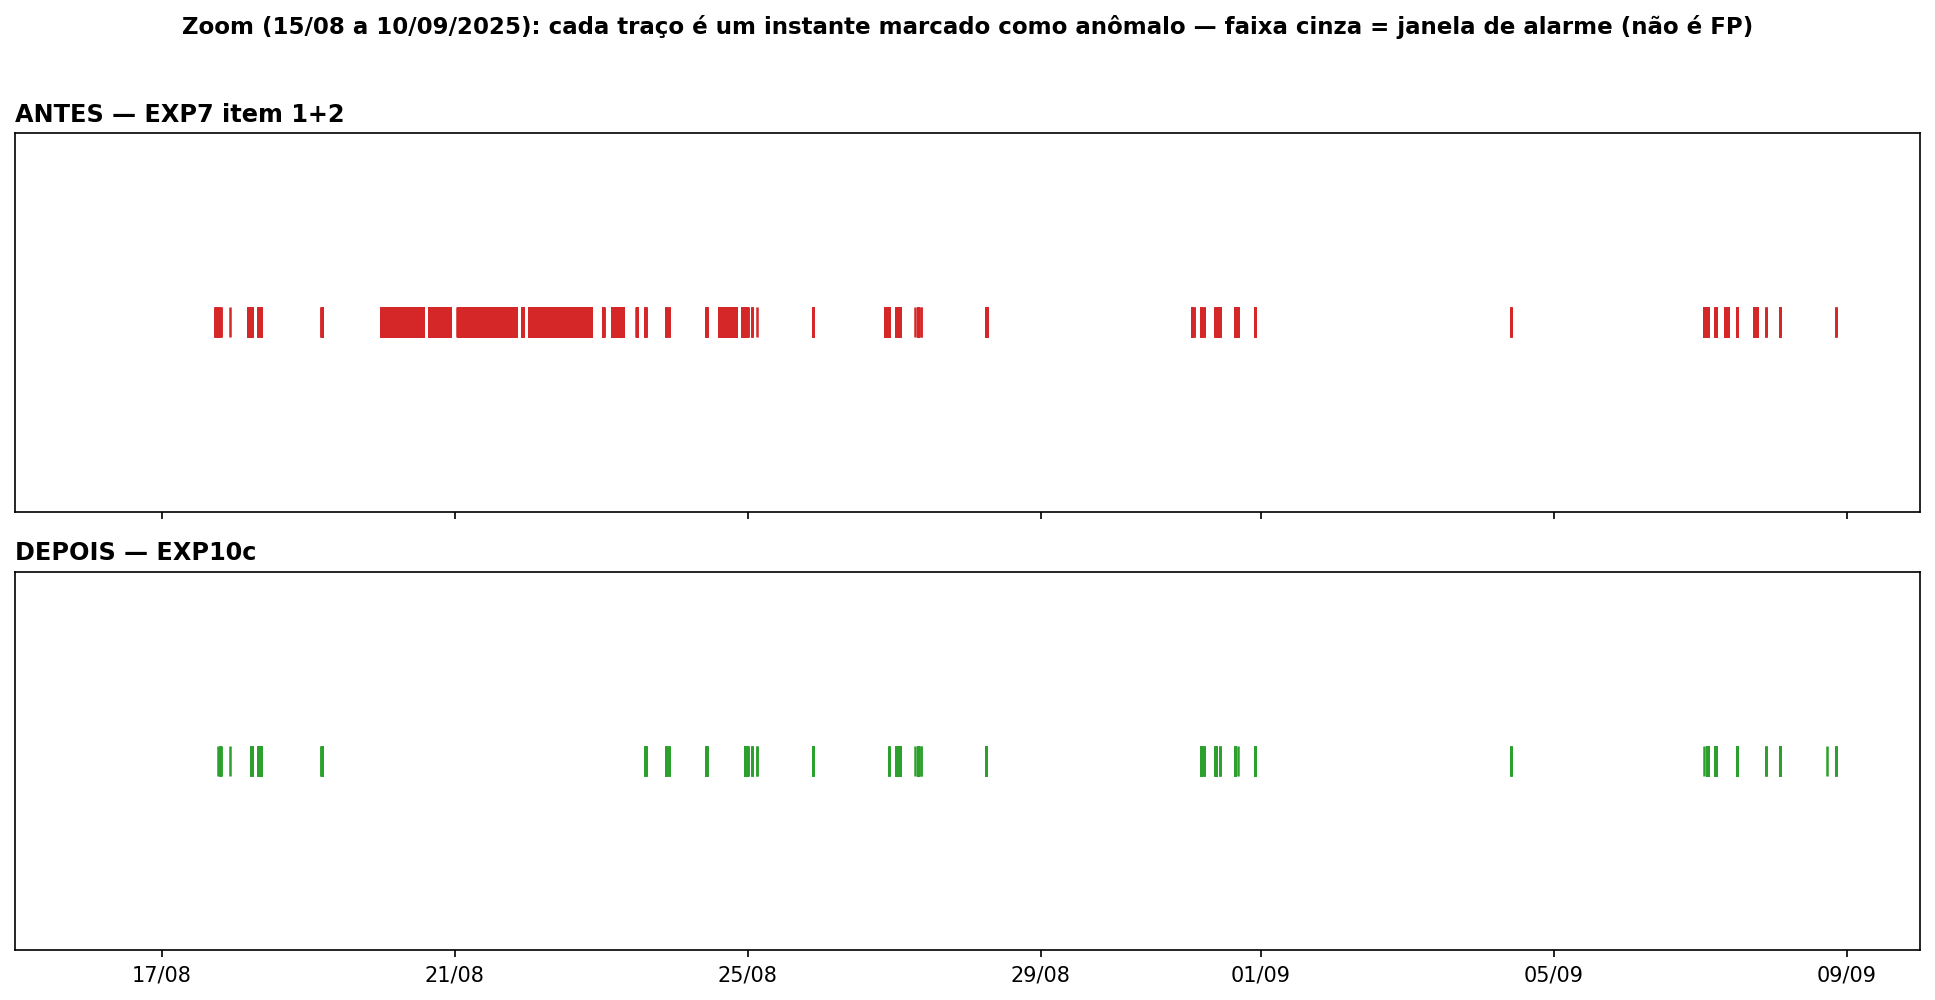
\includegraphics[width=\textwidth]{figs/exp10/09_zoom_antes_depois.png}
\caption{Zoom num episódio específico (29/01/2026): 41 de 41 pontos de
falso alerta removidos pelos filtros, sem afetar nenhuma detecção real
próxima.}
\end{figure}

\begin{figure}[H]
\centering
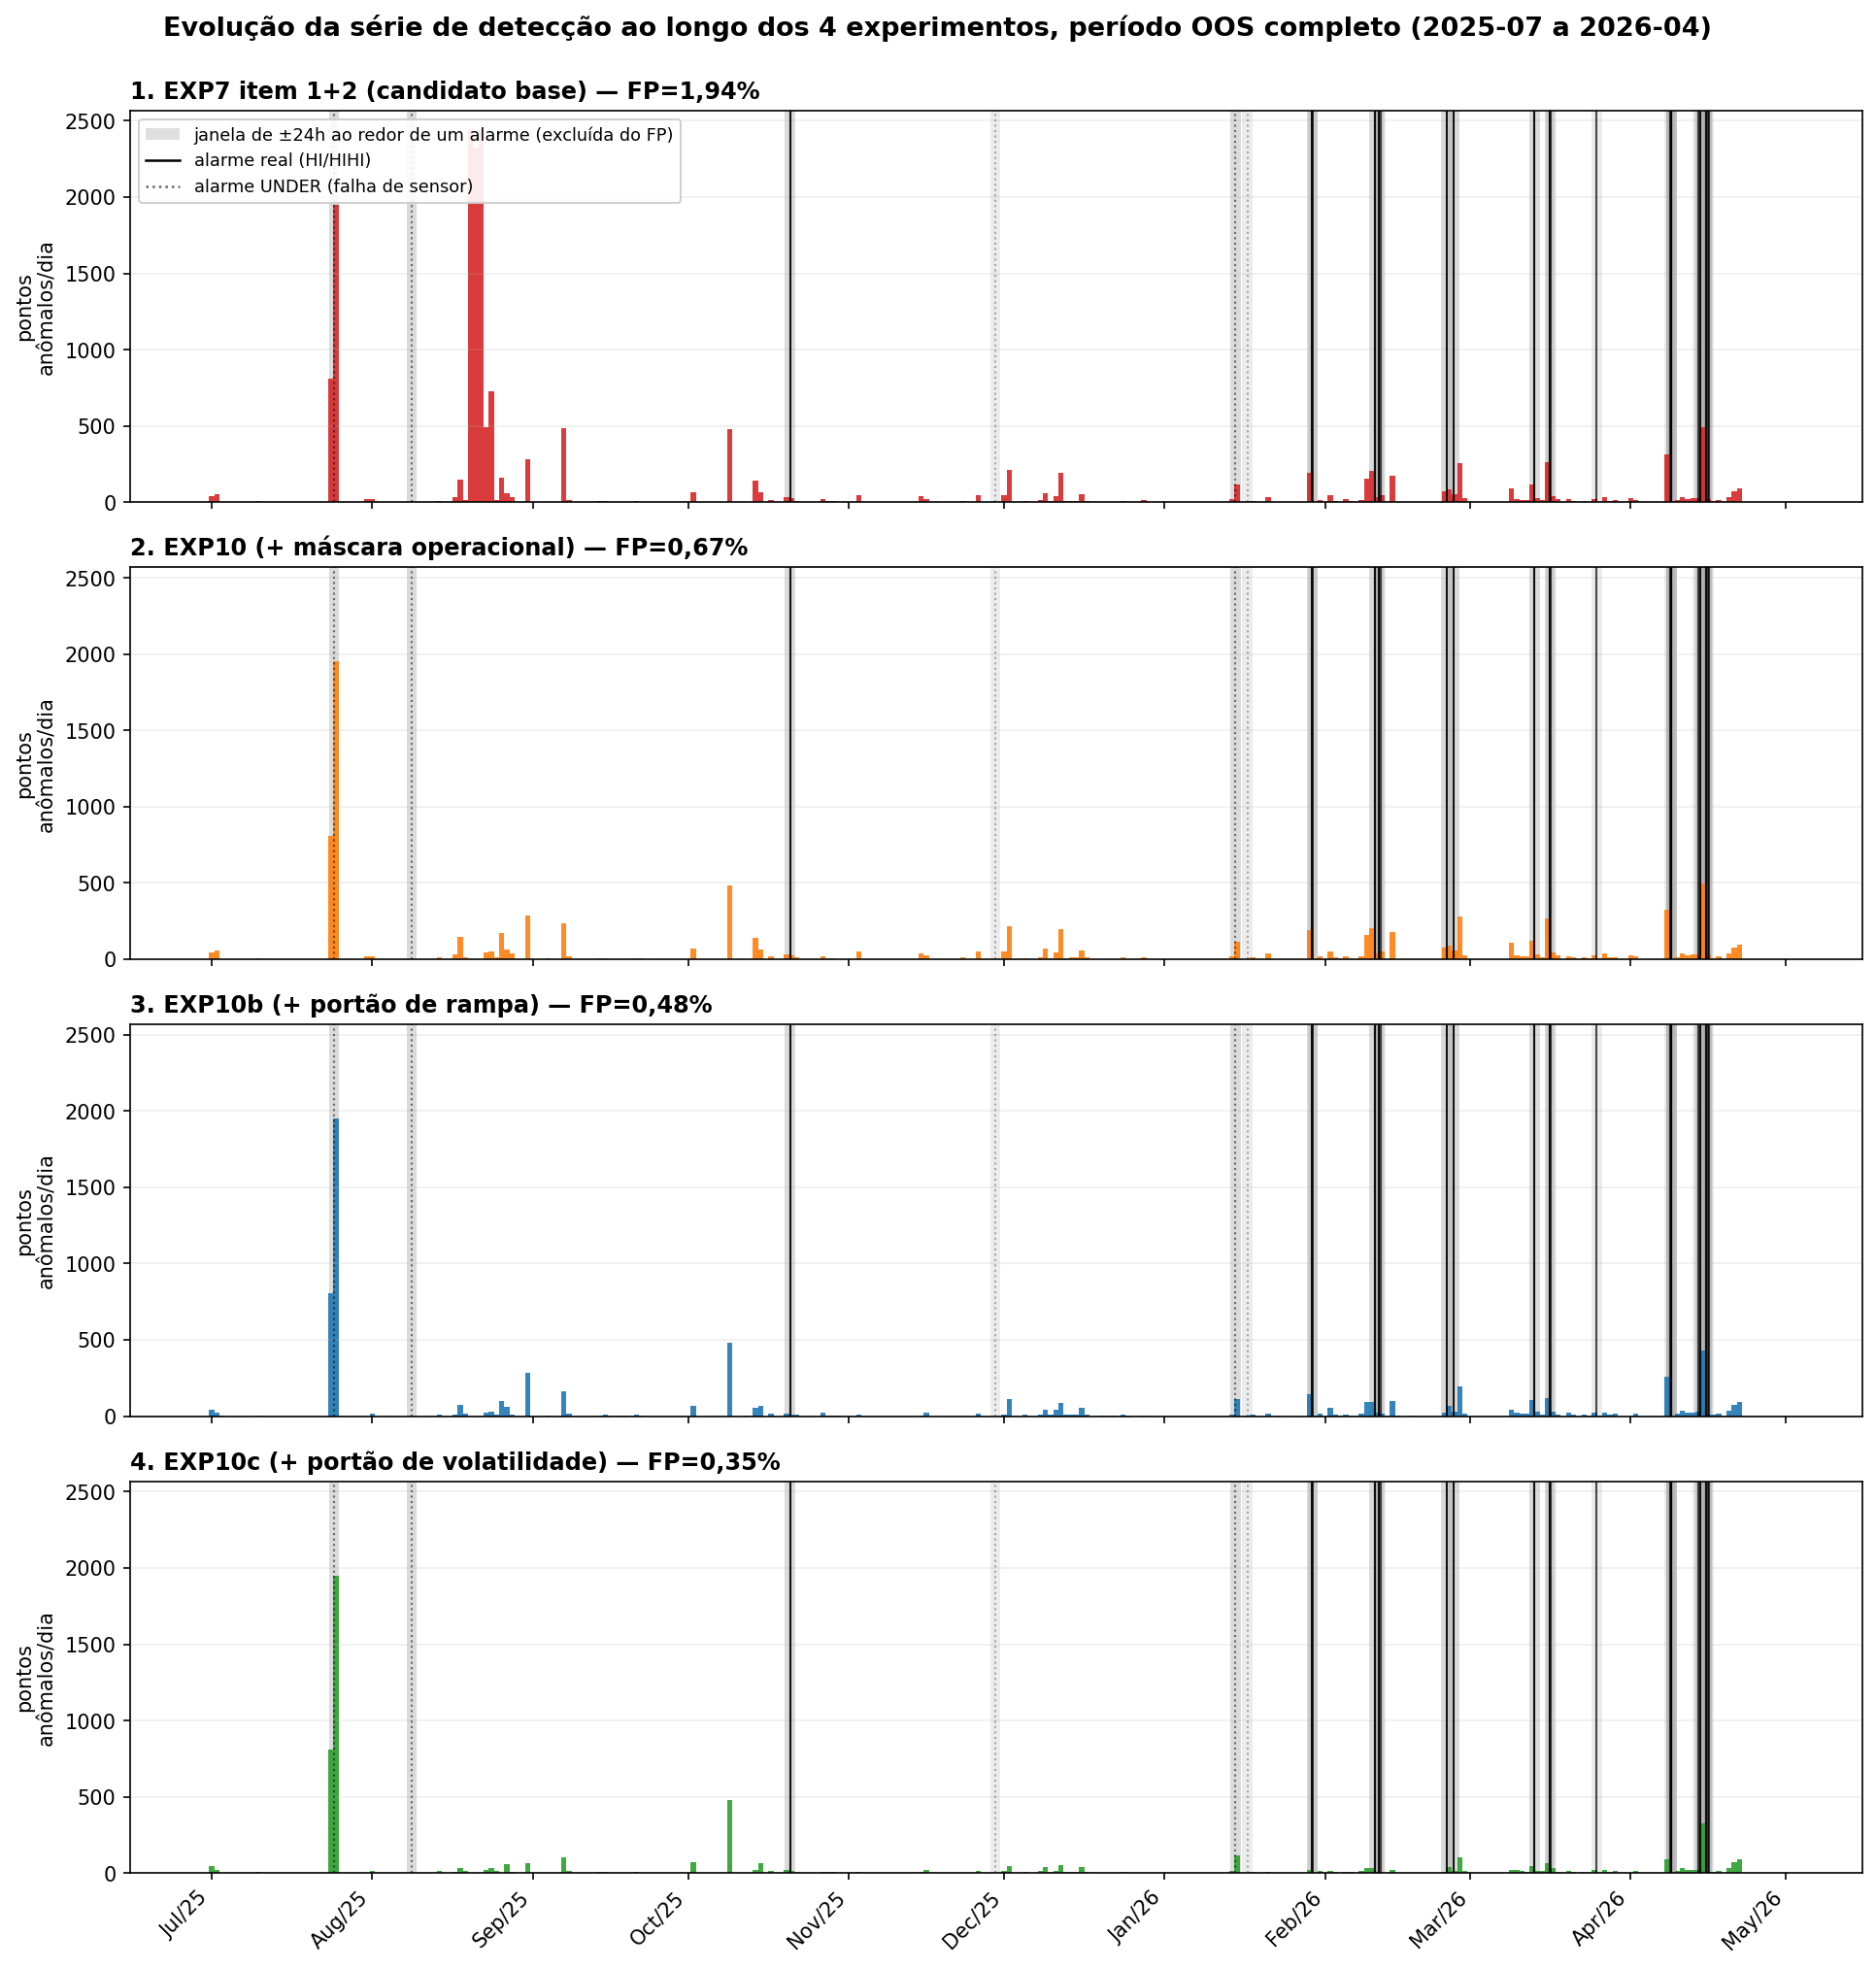
\includegraphics[width=\textwidth]{figs/exp10/11_evolucao_4_experimentos.png}
\caption{Evolução do falso alerta ao longo das 4 etapas (base, EXP10,
EXP10b, EXP10c) -- queda monotônica, sem retrocesso.}
\end{figure}

\begin{figure}[H]
\centering
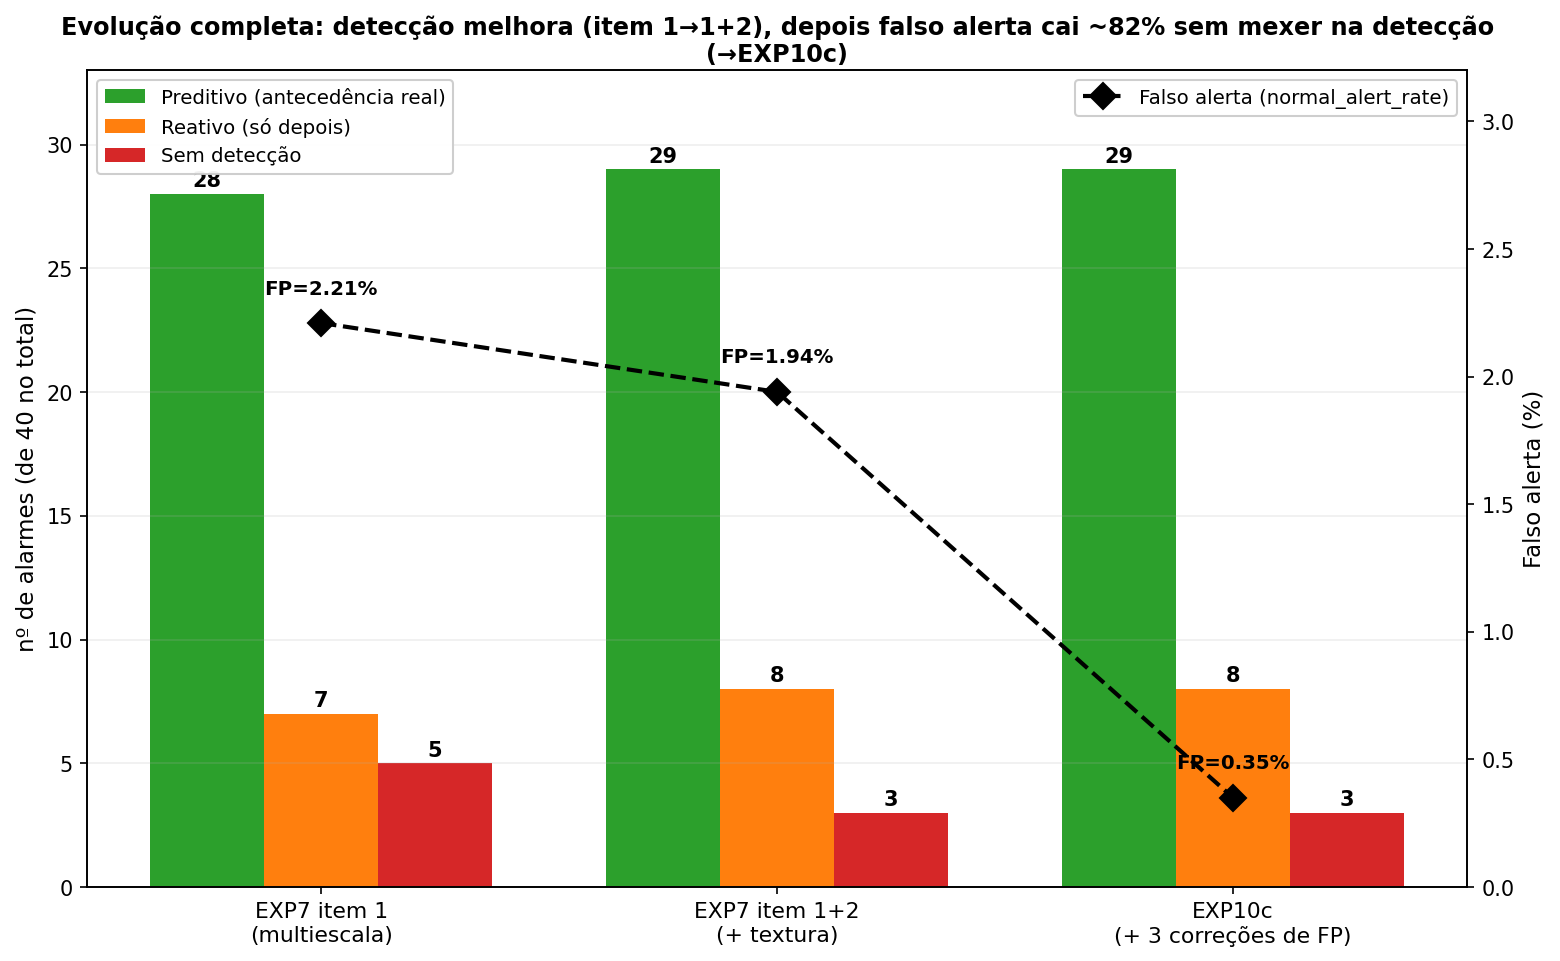
\includegraphics[width=\textwidth]{figs/exp10/15_evolucao_completa_deteccao_fp.png}
\caption{Visão consolidada: detecção (constante) e falso alerta
(decrescente) lado a lado ao longo de toda a série EXP10.}
\end{figure}

\subsection*{O que ainda resta (não endereçado nesta parte)}

\begin{itemize}
  \item $\sim$9,7\% do FP original coincide com outro alarme real do
        catálogo completo (pressão/partida a gás) -- fora do escopo de
        avaliação de 2 sensores, não é falso alerta genuíno, mas não foi
        corrigido.
  \item Resíduo de falha de sensor pontual ($\sim$2,1\%) que contamina a
        feature de tendência de 24h -- nenhuma das três correções mira
        esse mecanismo.
\end{itemize}

\clearpage
% =====================================================================
\part{Conclusão: a escada completa}
% =====================================================================

\section{A jornada em uma figura}

\begin{figure}[H]
\centering
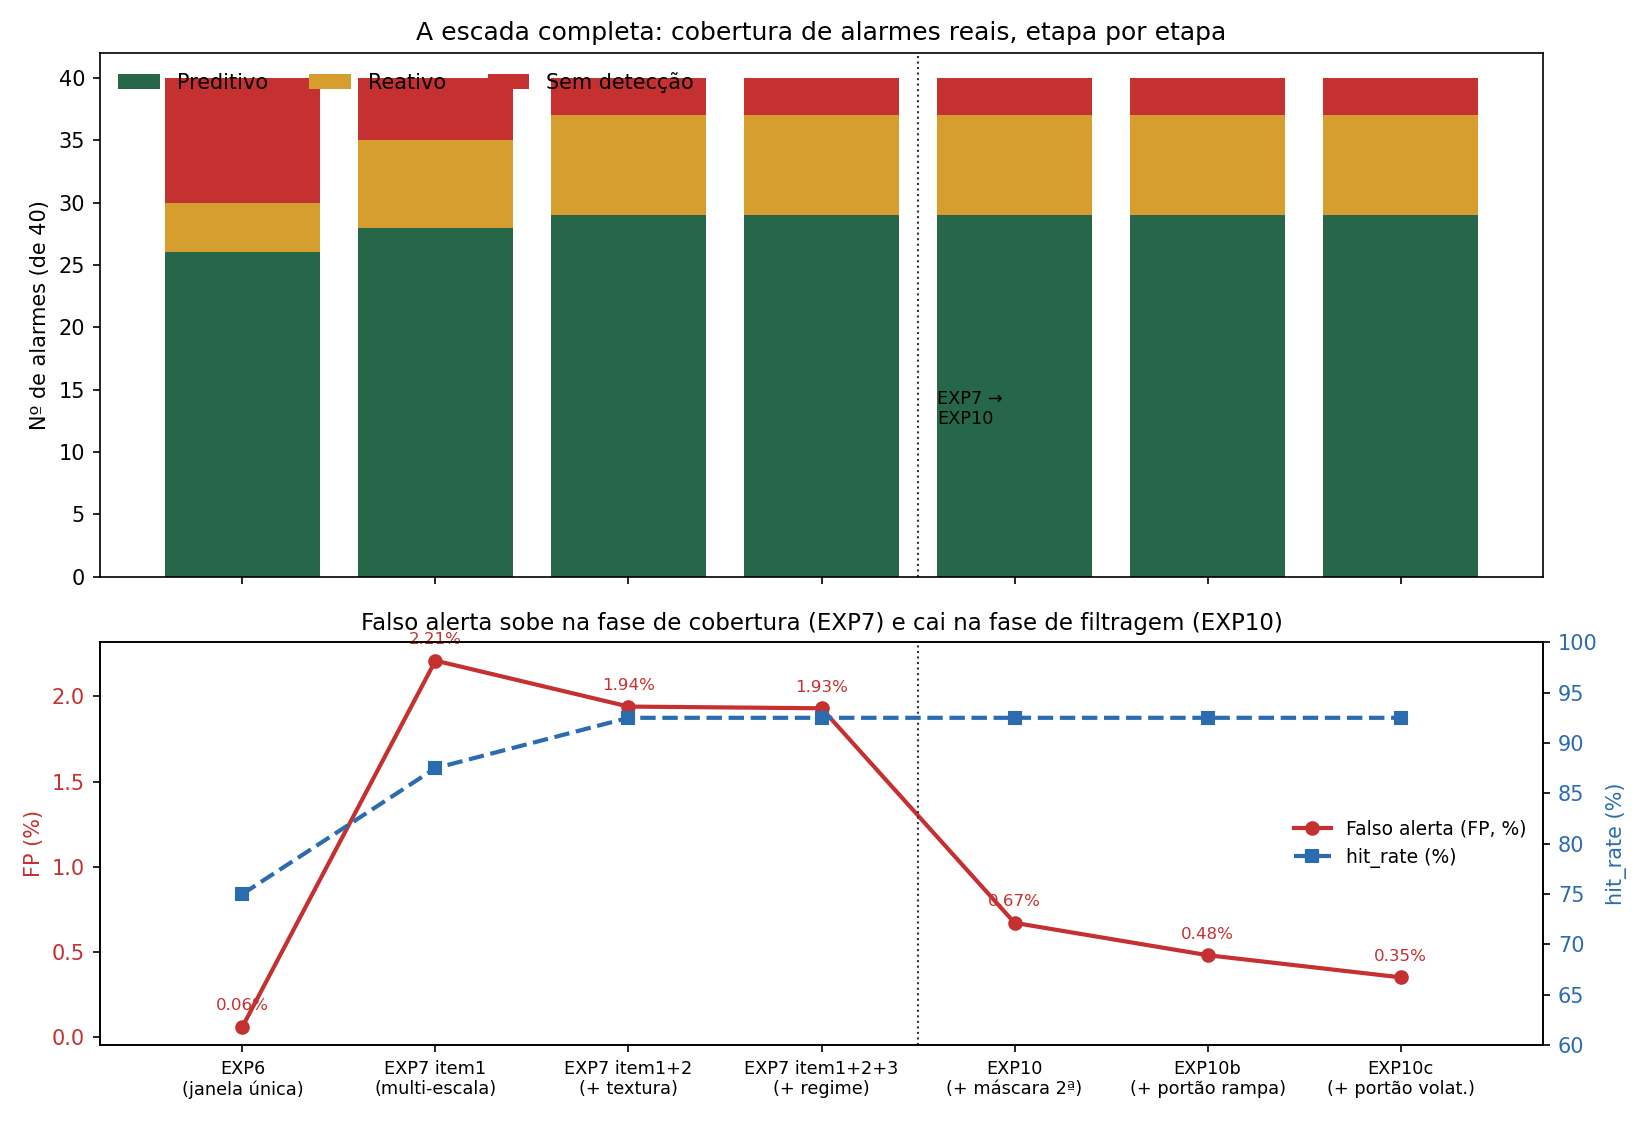
\includegraphics[width=\textwidth]{figs/escada_completa_exp6_exp10c.png}
\caption{As sete etapas, do EXP6 ao EXP10c, num só gráfico. Painel
superior: cobertura de alarmes (preditivo/reativo/sem detecção) --
melhora na fase EXP7 e se estabiliza na fase EXP10. Painel inferior: falso
alerta sobe na fase de cobertura (engenharia de features aumentando o
espaço de busca) e cai na fase de filtragem (mecanismos de supressão
pós-modelo) -- sem custo de detecção na segunda fase.}
\end{figure}

\section{Contexto geral vs.\ sensor-alvo}

Duas leituras complementares desta jornada:

\begin{itemize}
  \item \textbf{Contexto geral (métricas agregadas):} hit\_rate subiu de
        75,0\% para 92,5\% (65,0\%$\to$90,6\% olhando só alarmes
        fisicamente genuínos, sem os UNDER); falso alerta teve uma curva
        em U -- subiu de 0,06\% para 2,21\% na fase de cobertura (EXP7),
        e caiu de 1,94\% para 0,35\% na fase de filtragem (EXP10), \emph{sem
        nunca sacrificar} nenhum dos 37 alarmes já capturados.
  \item \textbf{Sensor-alvo (casos individuais):} os painéis de
        preditivo/reativo/sem-detecção (Figuras \ref{fig:pred-item2} e
        seguintes) e as séries antes/depois do EXP10
        (Figura~\ref{fig:serie-antes-depois}) mostram a mesma história em
        nível de evento -- alarmes específicos que passam de ``sem
        detecção'' para ``preditivo'' conforme a engenharia de features
        evolui, e episódios de falso alerta específicos que desaparecem
        da série do sensor-alvo conforme os filtros de pós-processamento
        entram, sem apagar nenhum ponto vermelho legítimo.
\end{itemize}

\section{Onde isso deixa o detector}

\begin{table}[H]
\centering
\small
\begin{tabular}{@{}lccc@{}}
\toprule
\textbf{Etapa} & \textbf{hit\_rate} & \textbf{FP} & \textbf{Antecedência mediana} \\
\midrule
EXP6 (baseline, janela única) & 75,0\% & 0,06\% & 12,4h \\
EXP7 item1 (multi-escala) & 87,5\% & 2,21\% & 15,0h \\
EXP7 item1+2 (+ textura) & 92,5\% & 1,94\% & 14,7h \\
EXP7 item1+2+3 (+ regime) & 92,5\% & 1,93\% & 14,7h \\
EXP10 (+ máscara secundária) & 92,5\% & 0,67\% & 14,7h \\
EXP10b (+ portão de rampa) & 92,5\% & 0,48\% & 14,7h \\
\textbf{EXP10c (+ portão de volatilidade)} & \textbf{92,5\%} & \textbf{0,35\%} & \textbf{14,7h} \\
\bottomrule
\end{tabular}
\caption{A escada completa. Sobre os 32 alarmes fisicamente genuínos
(excluindo UNDER, Seção~\ref{sec:qualidade}), a cobertura real é de
90,6\% (29/32) desde o item 1+2 em diante -- as etapas seguintes (item 3,
EXP10/10b/10c) preservam esse número e atacam exclusivamente o falso
alerta.}
\end{table}

\textbf{O que foi tentado depois e não trouxe ganho adicional} (fora do
escopo temporal deste relatório, ver \texttt{docs/analise\_automl\_exp10.md}
seção EXP12): re-otimizar o par percentil/debounce por cima dos 3 filtros
do EXP10c não encontrou margem real -- o piso de FP atual está nos dois
mecanismos ainda não endereçados (alarme cross-sensor fora do escopo de
avaliação, resíduo de sensor pontual), não no threshold do modelo.

\end{document}
